%! suppress = UnresolvedReference


\chapter{\app 的设计}\label{ch:design}


\section{项目的整体架构设计}\label{sec:arch-design}

\todo{增加宏观介绍,Pan-T等模块的划分。 https://github.com/CCXXXI/thesis/issues/82}

\subsection{Git子模块介绍}\label{subsec:git-submodule}

Git子模块(submodule)允许将一个Git仓库作为另一个Git仓库的子目录。为了方便项目管理,本项目的内容被拆分到了多个Git仓库,各个仓库之间的一些共享的部分使用了Git子模块来实现复用与同步。

与Git子模块功能类似的工具还有Git子树(subtree)等,但其他工具对于在主仓库修改之后向子仓库进行推送的这一需求都没有像Git子模块这样的良好支持,再考虑到整个项目架构的一致性,本项目在内部各个仓库之间的依赖方式上都选择了Git子模块作为解决方案(对外部仓库的依赖方式则有所不同)。

\subsection{项目包含的Git仓库}\label{subsec:git-repositories}

本项目在整体架构上一共由7个Git仓库组成,这些仓库的名称以及仓库之间的子模块关系如图~\ref{fig:repositories}所示。

\begin{figure}[ht]
    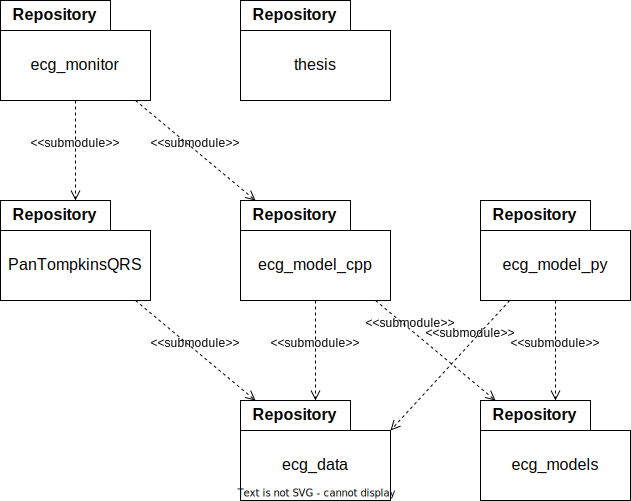
\includegraphics[width=\textwidth]{../assets/repositories.drawio}
    \bicaption{项目包含的Git仓库}{Git repositories of the project}
    \label{fig:repositories}
\end{figure}

\subsubsection{thesis}\label{subsubsec:repo-thesis}

这是本篇论文所在的仓库。论文本身作为项目文档的一部分,也被包含在本项目之中。该仓库包含论文的\LaTeX 源码,以及论文中引用的图片等资源文件,还有自动格式化、依赖版本管理、自动构建测试、自动发布新版本等持续集成配置。

论文与应用本身的代码是分离的,所以论文的仓库与应用的仓库之间没有任何子模块关系。此外,论文仓库以Git子树的形式包含了论文模板\footnote{\url{https://github.com/Koyamin/ECNUThesis-Undergraduate}},没有使用Git子模块是因为基于模板进行编写后只需要直接提交至主仓库,不需要向子仓库推送,这与~\ref{subsec:git-submodule} 节所述的情况不同。

\subsubsection{ecg\_monitor}\label{subsubsec:repo-monitor}

这是应用的主体仓库。该仓库包含基于Flutter框架编写的Dart代码,以及相关的各种配置文件等。仓库的命名与应用的包名一致,因此按照Dart对包名的相关限制使用了小写下划线的命名风格,而非Git仓库常用的小写连字符。为了保持项目各个仓库之间的一致性,其他仓库(除PanTompkinsQRS外)也都使用了小写下划线的命名风格。

为了方便调用C++代码,该仓库以Git子模块的形式包含了PanTompkinsQRS和ecg\_model\_cpp两个子仓库,这两个子仓库分别提供了Pan-Tompkins算法和基于LibTorch的心电图智能分析算法的实现。

\subsubsection{PanTompkinsQRS}\label{subsubsec:repo-qrs}

这是应用中用于实现Pan-Tompkins算法的仓库。该仓库是rafaelmmoreira编写的Pan-Tompkins算法的C语言实现\footnote{\url{https://github.com/rafaelmmoreira/PanTompkinsQRS}}的复刻(fork),在原始版本的基础上根据项目需要进行了一些修改。出于对原作者的尊重,该仓库的名称与原作者的命名保持一致,因此与项目内其他仓库的命名风格不同。

该仓库被ecg\_monitor所包含,并且为了方便测试而将ecg\_data包含为了子仓库,后者提供了一些测试用的心电图数据,用作测试时的输入。

\subsubsection{ecg\_model\_cpp}\label{subsubsec:repo-cpp}

这是应用中用于实现基于LibTorch的心电图智能分析算法的仓库。该仓库是ecg\_model\_py仓库的C++实现,使用了LibTorch作为框架。

该仓库被ecg\_monitor所包含,且包含了ecg\_data作为测试输入数据,还包含了ecg\_models作为与ecg\_model\_py共享的模型文件以及测试预期输出。

\subsubsection{ecg\_model\_py}\label{subsubsec:repo-py}

这是基于PyTorch实现的心电图智能分析算法的所在仓库。该仓库以算法的原始版本作为初始提交,在此基础上根据项目需要进行了修改。

Python版本的算法并不直接被应用调用,因此该仓库不是其他仓库的子模块。该仓库包含了ecg\_data作为测试输入数据,将与ecg\_model\_cpp共享的模型文件保存在ecg\_models,并将PyTorch版本的算法输出也写入ecg\_models子模块以便与ecg\_model\_cpp共享。

\subsubsection{ecg\_data}\label{subsubsec:repo-data}

该仓库存储了各算法仓库用作测试输入的心电图数据,以及从公开数据库下载心电数据并转换格式的相关代码。该仓库中的数据由仓库内的代码写入,被上述三个算法仓库所读取。

\subsubsection{ecg\_models}\label{subsubsec:repo-models}

该仓库存储了TorchScript模型文件,以及模型在测试输入下的输出结果。该仓库的内容由ecg\_model\_py写入,被ecg\_model\_cpp读取。因为模型文件较大(60多MB),且不被Pan-Tompkins算法所需要,所以该仓库与ecg\_data进行了分离。


\section{应用的界面与功能设计}\label{sec:app-design}

\subsection{应用的界面设计规范}\label{subsec:app-design-spec}

本应用与其他同类应用的一大差别在于其遵循专业的设计规范对应用界面进行了严格的设计。

应用整体上遵循Material 3设计规范\cite{MaterialDesign}。Material 3(也称为Material You)是Google在2021年5月的Google I/O大会上宣布的新一代Material设计规范,和前代规范相比具有从用户的壁纸自动生成动态主题颜色、按钮更大、界面动画更多等新特性,并在其他一些细节设计上有所优化。目前Material 3设计已被广泛应用于Google的各种应用程序,并成为Android应用的推荐设计规范。

尽管Material 3按照Google的设计是可以在任何平台(包括iOS)上使用的,但从事实上来说,iOS应用确实较少使用Material风格的设计,而较多按照苹果的推荐遵循Cupertino\footnote{苹果官方并未给自己的设计规范进行像Material这样的明确命名,Cupertino这个名字是Flutter在其文档中使用的,可能是基于苹果总部位于美国加利福尼亚州丘珀蒂诺(Cupertino)市的事实。}设计。为了符合iOS平台的用户习惯,本应用在iOS平台上将部分UI组件替换为了iOS应用常用的Cupertino风格的组件。由于Cupertino并未像Material一样提供全平台可用的设计,所以应用的设计仍然以Material为主,在Android平台上完全使用Material 3风格的设计,而在iOS平台上则使用Material 3风格与Cupertino风格的混合设计,如图~\ref{fig:android-ios} 所示。

\begin{figure}[ht]
    \subcaptionbox{Android}{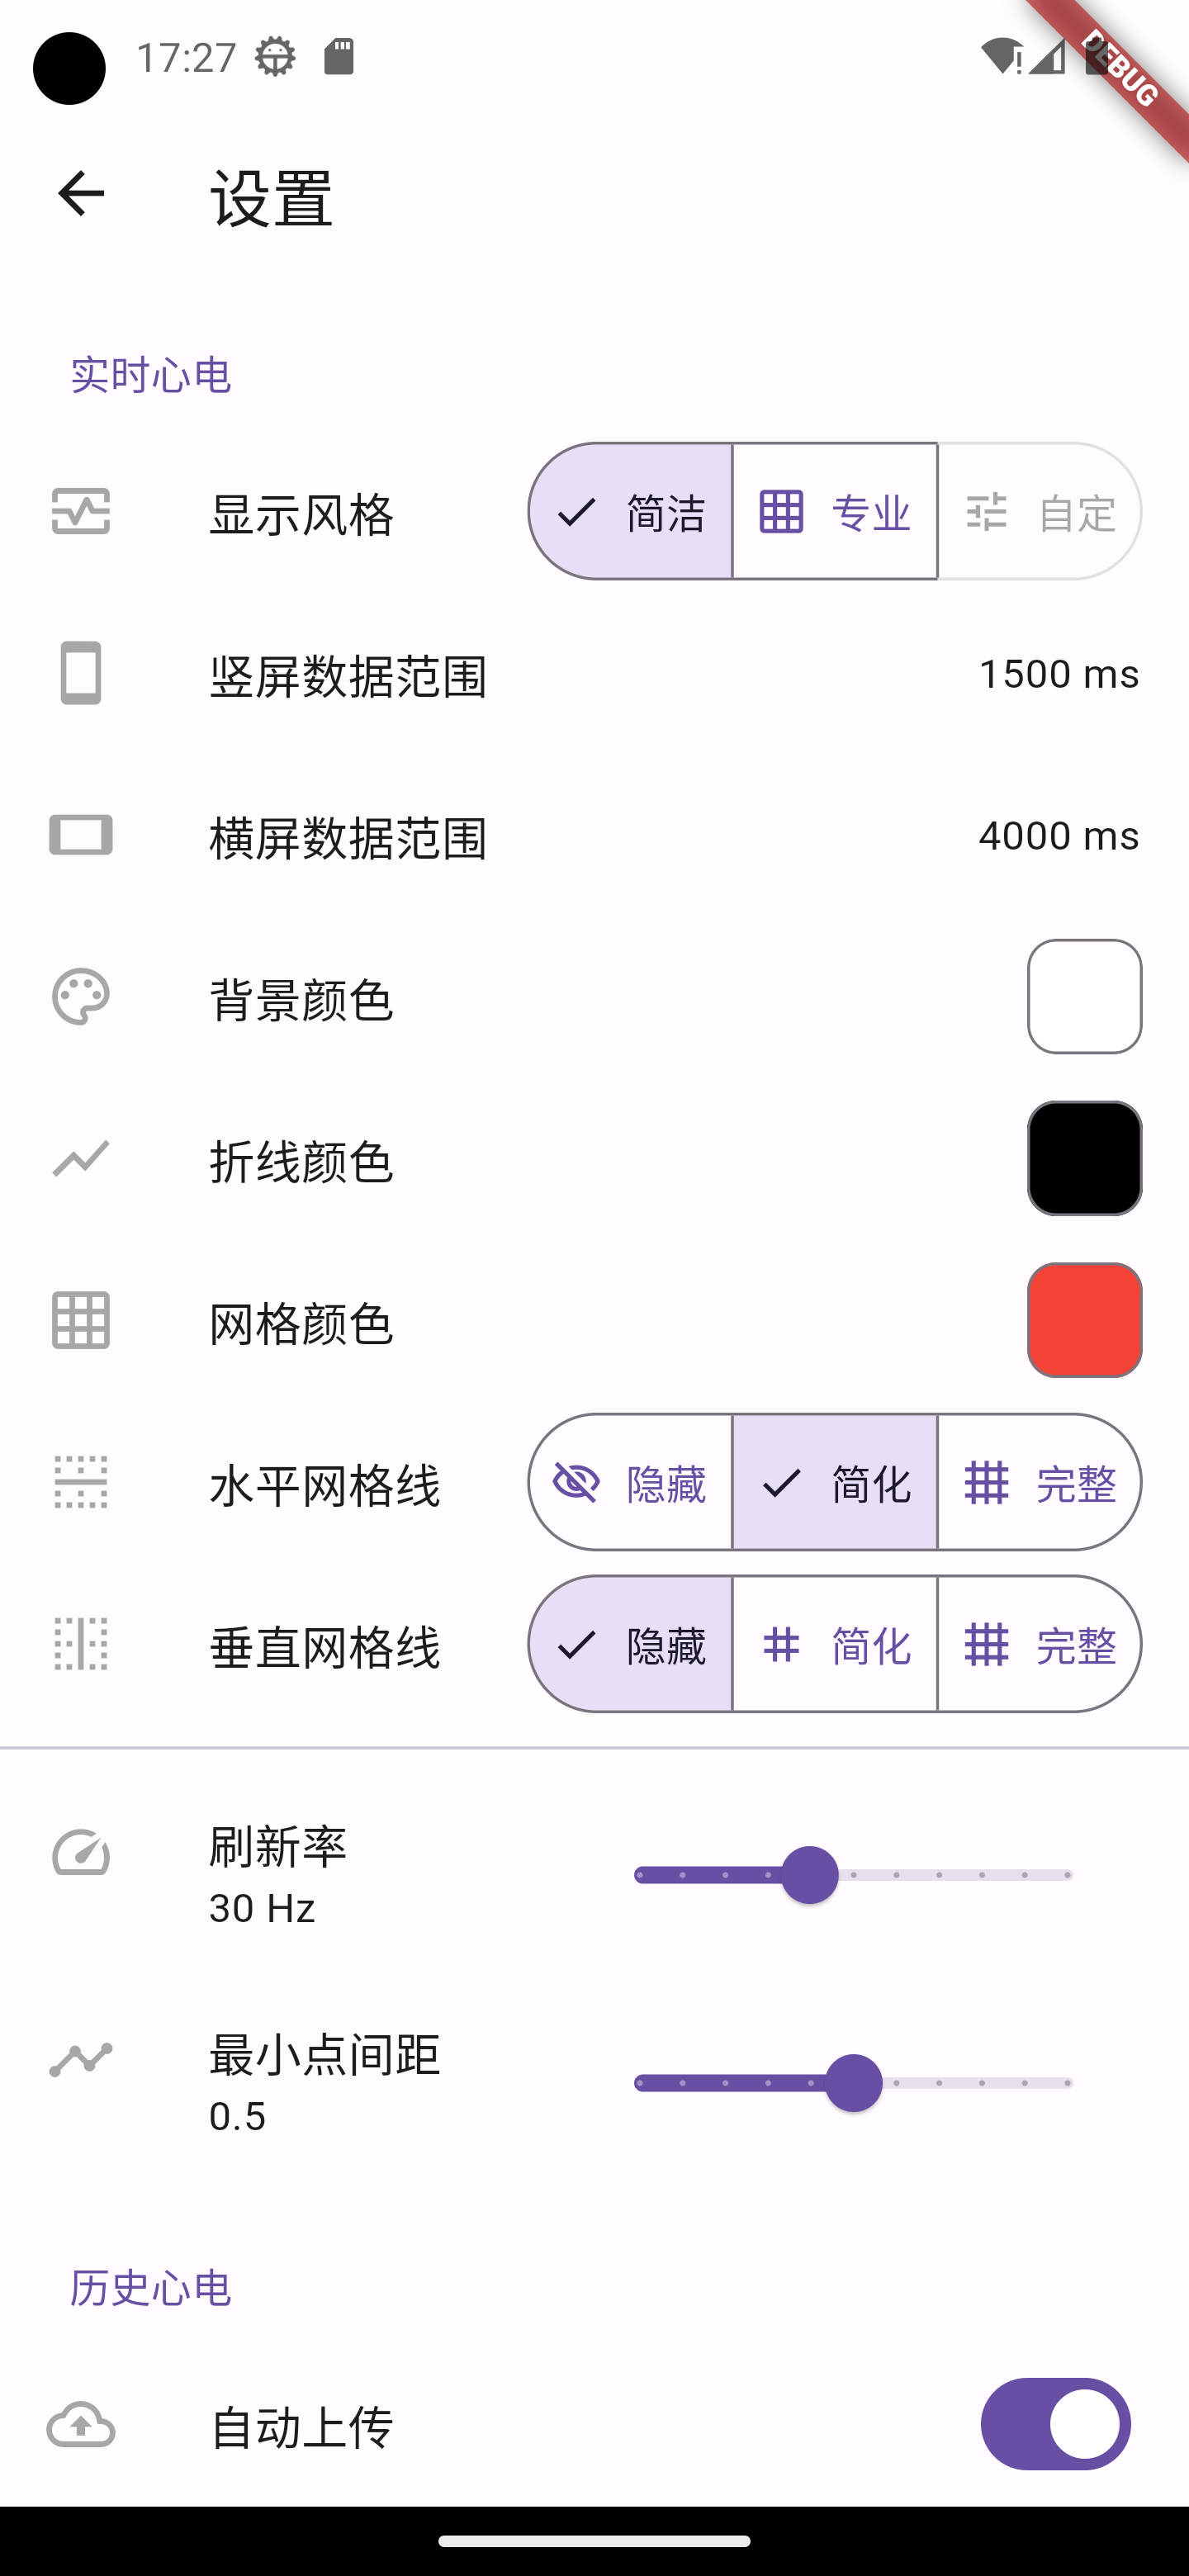
\includegraphics[height=17cm]{../assets/settings}}
    \subcaptionbox{iOS}{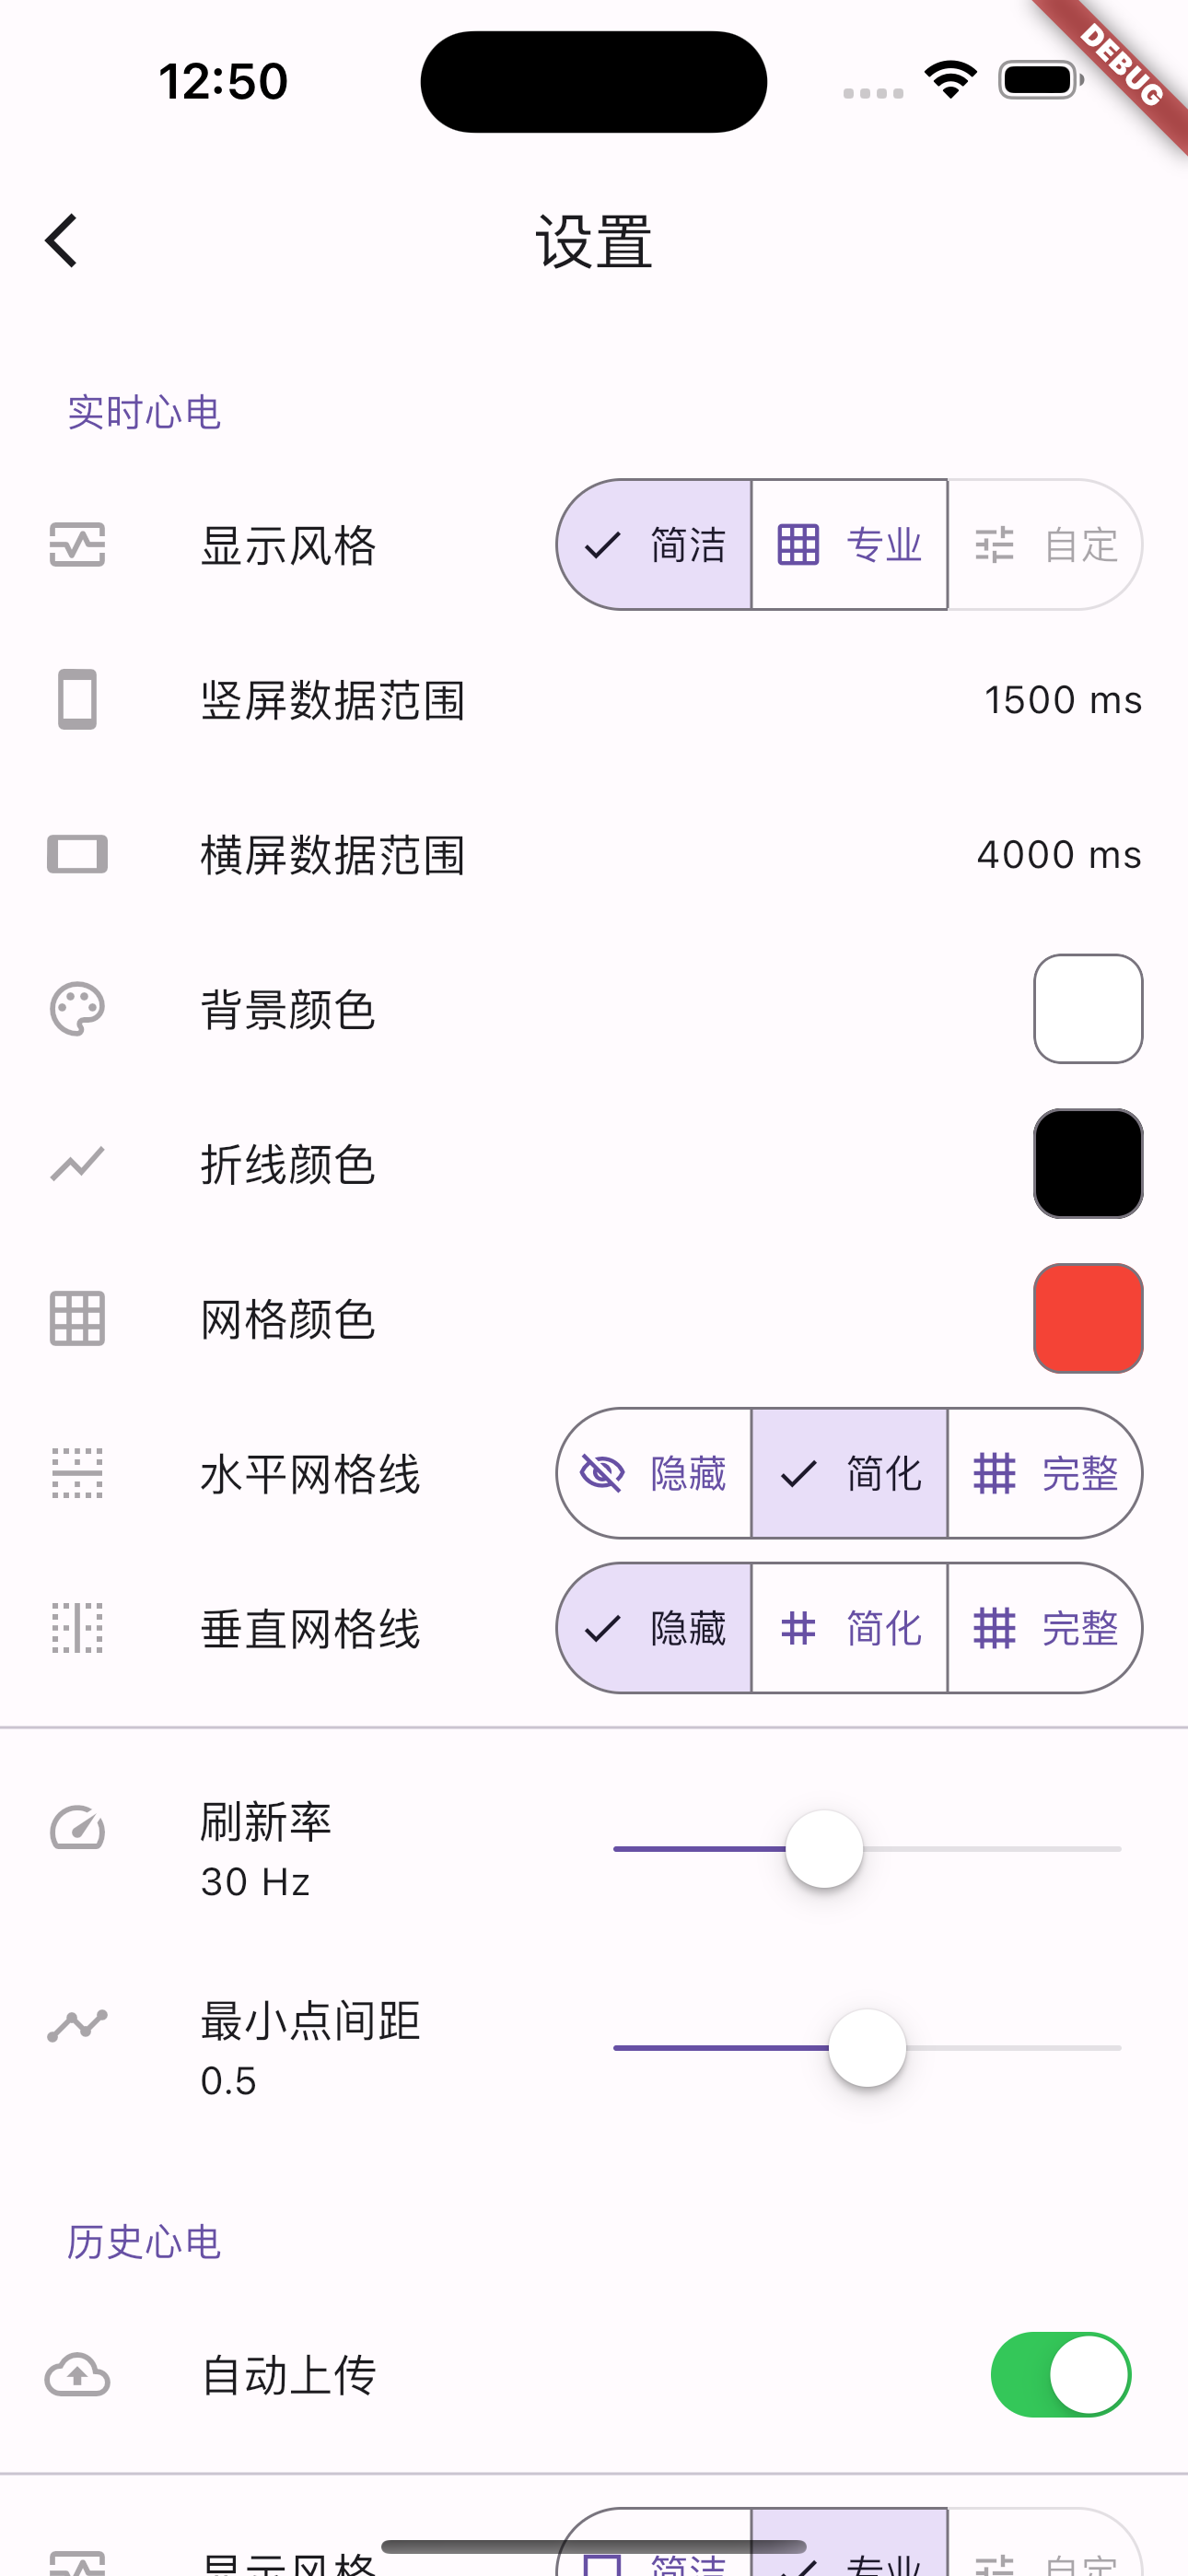
\includegraphics[height=17cm]{../assets/ios-settings}}
    \bicaption{应用在Android和iOS平台上的界面设计对比}{Comparison of the app's UI design on Android and iOS}
    \label{fig:android-ios}
\end{figure}

从图~\ref{fig:android-ios} 中可以看出应用在Android平台与iOS平台上的界面设计的一些差异,包括标题的对齐方式(Android居左,iOS居中)、左上角返回按钮的图标(Android使用完整箭头,iOS使用仅有头部的简化箭头)、滑动条与切换按钮的外观(按照各自规范中的相关要求)、文本的字体(iOS的字体更细)等。

\subsection{实时心电界面的设计}\label{subsec:real-time-design}

实时心电界面的整体设计如图~\ref{fig:real-time} 所示。

\begin{figure}[ht]
    \subcaptionbox{心率检测中}{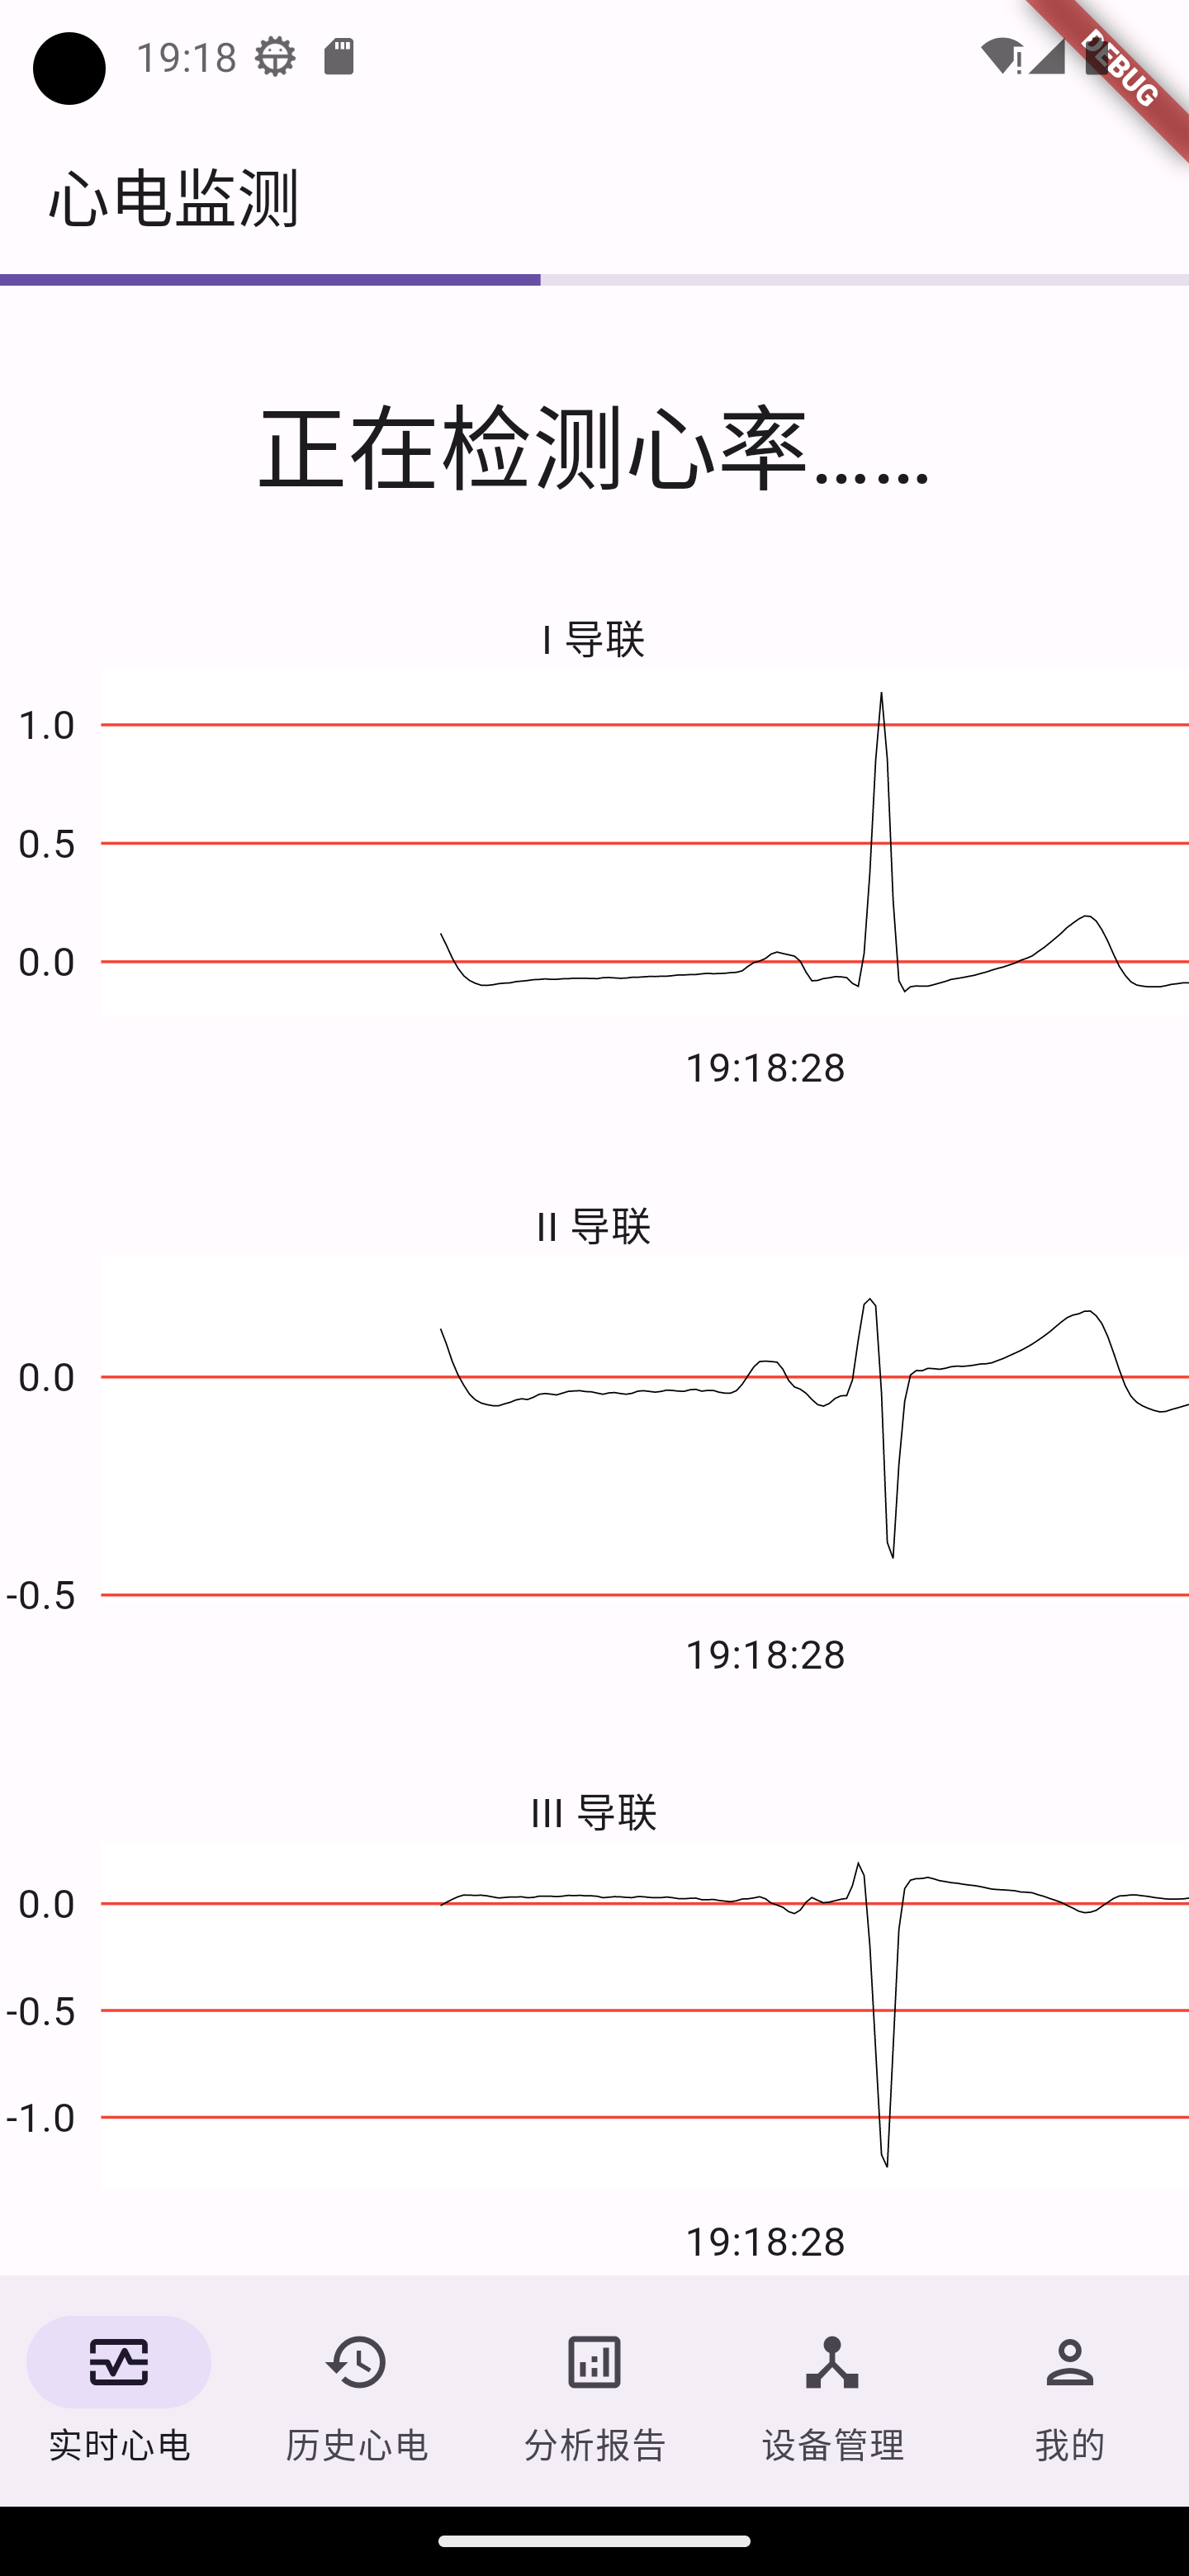
\includegraphics[width=.33\textwidth]{../assets/real-time-learning}}
    \subcaptionbox{正常状态}{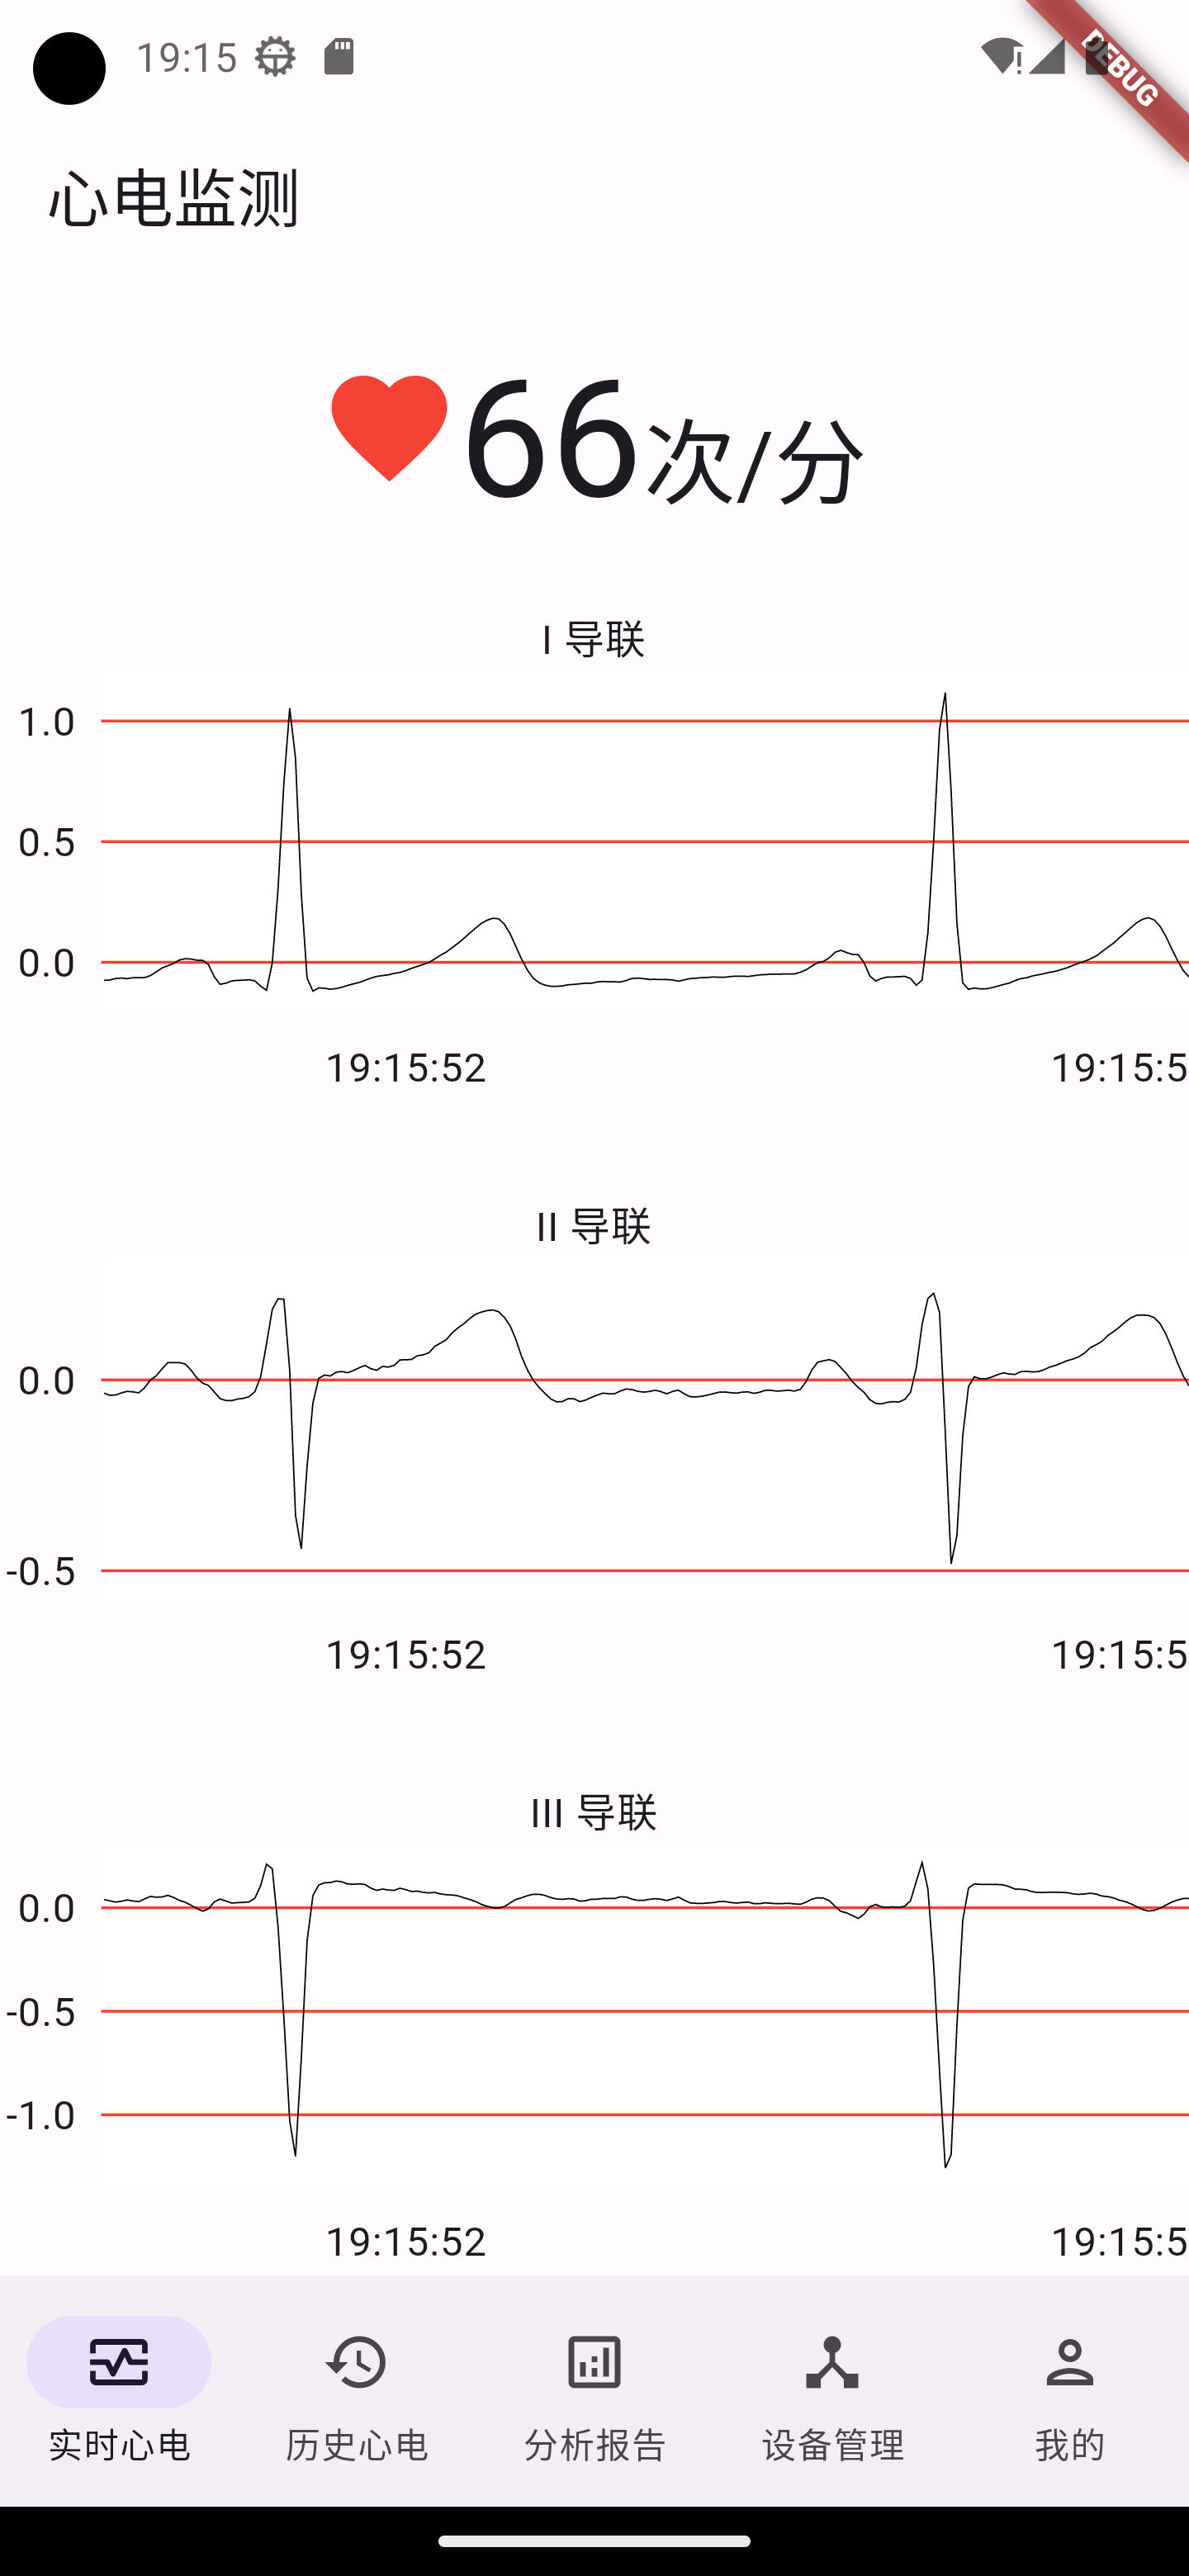
\includegraphics[width=.33\textwidth]{../assets/real-time}}
    \subcaptionbox{设备未连接}{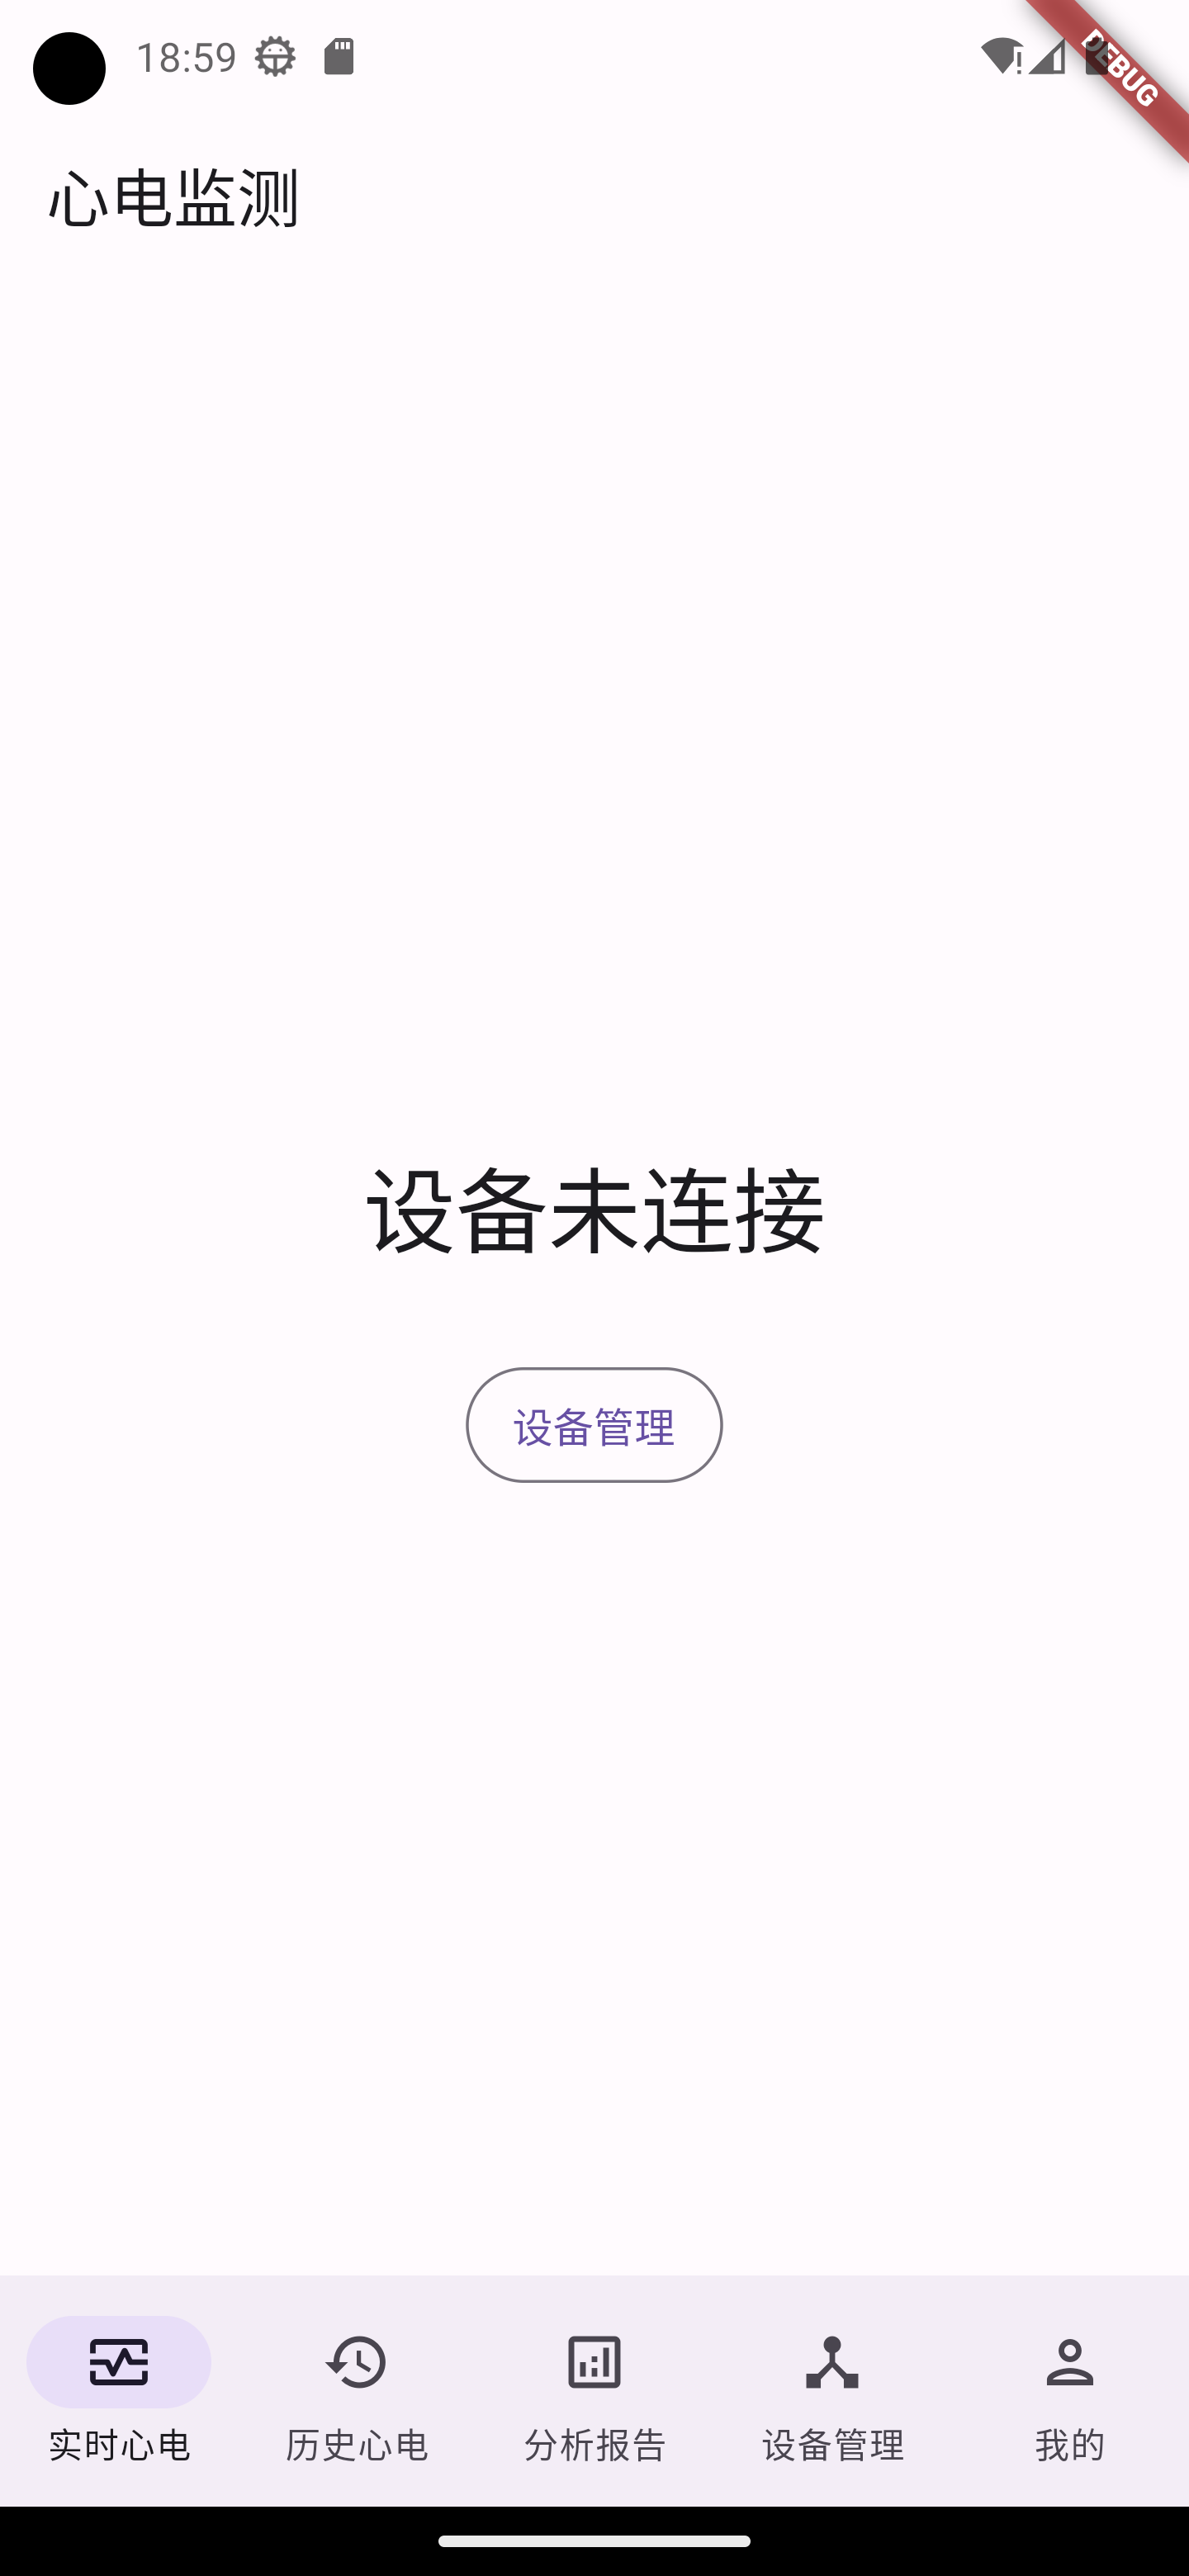
\includegraphics[width=.33\textwidth]{../assets/real-time-na}}
    \bicaption{实时心电界面的设计}{Design of the real-time ECG page}
    \label{fig:real-time}
\end{figure}

实时心电界面的主体可以分为心率和心电图两大部分。另外,在整个应用的最上方显示了应用的名称,最下方显示了应用的导航栏,导航栏提供了应用中最主要的几个界面的入口。

\subsubsection{心率部分的设计}\label{subsubsec:heart-rate-design}

实时心电界面的上方显示了用户当前的心率。

当用户刚刚佩戴上或连接上心电监测设备的时候,由于缺少数据,心率无法立即获得。在这种状态下,心率部分会显示“正在检测心率……”作为占位符,并且上方会显示一个线状的进度条。Material规范中规定了两种类型的线状进度条,分别表示确定的和不确定的进度。因为心率检测所需的时间可以大致确定,所以此处使用了确定进度的版本,进度条的已填充长度占比表示心率检测的预测进度。进度条的使用可以向用户提供检测进度的视觉反馈,虽然并不能在实际上加快检测速度,但由于减少了不确定性,仍然可以减少用户在等待过程中的焦虑感与沮丧感,起到了与加快检测速度类似的作用。反之,如果在系统正在工作的过程中不为用户提供指示,比如某些网站在上传作业文件时的设计,即使是在只需要等待数秒的情况下,用户也会感到焦虑与沮丧,在更长时间后甚至会由于缺乏对任务最终可以完成的信心而感到挫折并放弃使用。进度条虽然只是个简单的组件,但对于软件的易用性和用户体验来说却是个关键设计。

心率检测的结果可用之后,该区域则会显示心率数据。显示内容由横向排布的三个组件组成:图标、数值和单位。图标使用了一个红色的心形标志,主要起到两个作用:一是指示该区域显示的内容是心率,由于应用的性质与该界面其他元素的暗示,用户很容易理解到所示数值表示心率,所以不需要使用文本等方式进行明确说明,只使用简单的图标已经足够;二是加强该区域的视觉强调效果,由于心率区域在整个屏幕上的面积占比较少,但重要性并不显著弱于下方的心电图等元素,所以使用了这个颜色较为鲜艳的图标来将用户的注意力吸引至该区域。数值和单位使用了不同大小的字体,数值较大而单位较小。这是因为心率数值是该区域的主要内容,且不断变动,需要较为强调。而心率的单位是固定的,不会变动,而且每分钟的次数(bpm)作为最常用的心率单位已经为用户所习惯,不需要特别强调,所以使用较小的字体弱化了单位的视觉效果,以突出其他部分。三个组件在横向与纵向上整体居中,内部按文本基线对齐(即靠下对齐)。

此外,整个心率显示区域在实时心电界面上的高度占比是固定的,以免在检测完成前后以及数值变动时引起下方心电图位置的上下移动。

\subsubsection{心电图部分的设计}\label{subsubsec:ecg-design}

心电图部分的设计参考了医学上常用的心电图纸的设计。心电图纸的整体外观在\nameref{ch:intro}部分的图~\ref{fig:ecg-paper-example} 中已经展示过,这里对其具体布局方式进行一些补充介绍。

心电图纸包含横纵交错的坐标线,通常为红色或浅红色,如图~\ref{fig:ecg-paper} 所示。每1mm一小格(用细线分隔),每5mm一大格(用粗线分隔)。横轴一小格表示40ms,一大格表示200ms。纵轴一小格表示0.1mV,一大格表示0.5mV。心电图的边缘有1mV(10mm高)的参考波形,并标注该条图像的导联名称。

\begin{figure}[ht]
    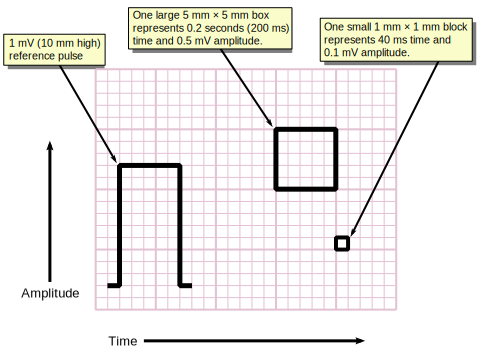
\includegraphics[width=\textwidth]{../assets/ECG_Paper_v2}
    \bicaption{心电图纸的布局}{Layout of ECG paper}
    \label{fig:ecg-paper}
\end{figure}

在应用内实时心电图的设计过程中,对心电图纸的元素进行了一些精简与修改。首先,由于移动设备的屏幕尺寸较小,将心电数据的显示范围进行了缩减,纵轴范围根据当前图中显示的心电数据自适应变动,以最大值加0.1mV作为上限,最小值减0.1mV作为下限。横轴范围则按照心电数据的常见电压范围进行了等比例调整,使其与纵轴比例可以保持近似对应,并在应用设置内增加了相关的选项供用户按需自行调整。之后,由于纵向坐标线在实时心电图的快速移动的过程中会产生视觉上的严重干扰,所以将其去除,改为在下方显示数据对应的时间;为了保持视觉上的协调,横轴坐标线去除了划分小格的细线,仅保留了0.5mV一条的粗线。最后,考虑到一般用户对心电图纸的参考波形的了解程度较低,加之移动设备的显示空间有限,所以将参考波形去除,改为在左侧显示电压数值,并相应地将导联名称移至心电图的正上方中央。

心电图部分在竖屏和横屏状态下有不同的显示方式。竖屏状态下,如之前所示,三个导联的心电图从上到下竖向排布在该区域。由于移动设备的屏幕宽度较窄,所以竖屏状态下可以显示的时长也较短,屏幕中每个导联通常只能显示一到两个心拍。虽然可以在应用设置中对显示时长进行调整,但在显示区域的宽度无法改变的情况下,显示更长时间的数据只能是以降低细节的可见程度为代价的。为了提供一种可以在不提高显示密度的情况下查看更长时间的数据的方式,应用在横屏状态下会改为仅显示单个导联的数据,如图~\ref{fig:real-time-landscape} 所示。

\begin{figure}[ht]
    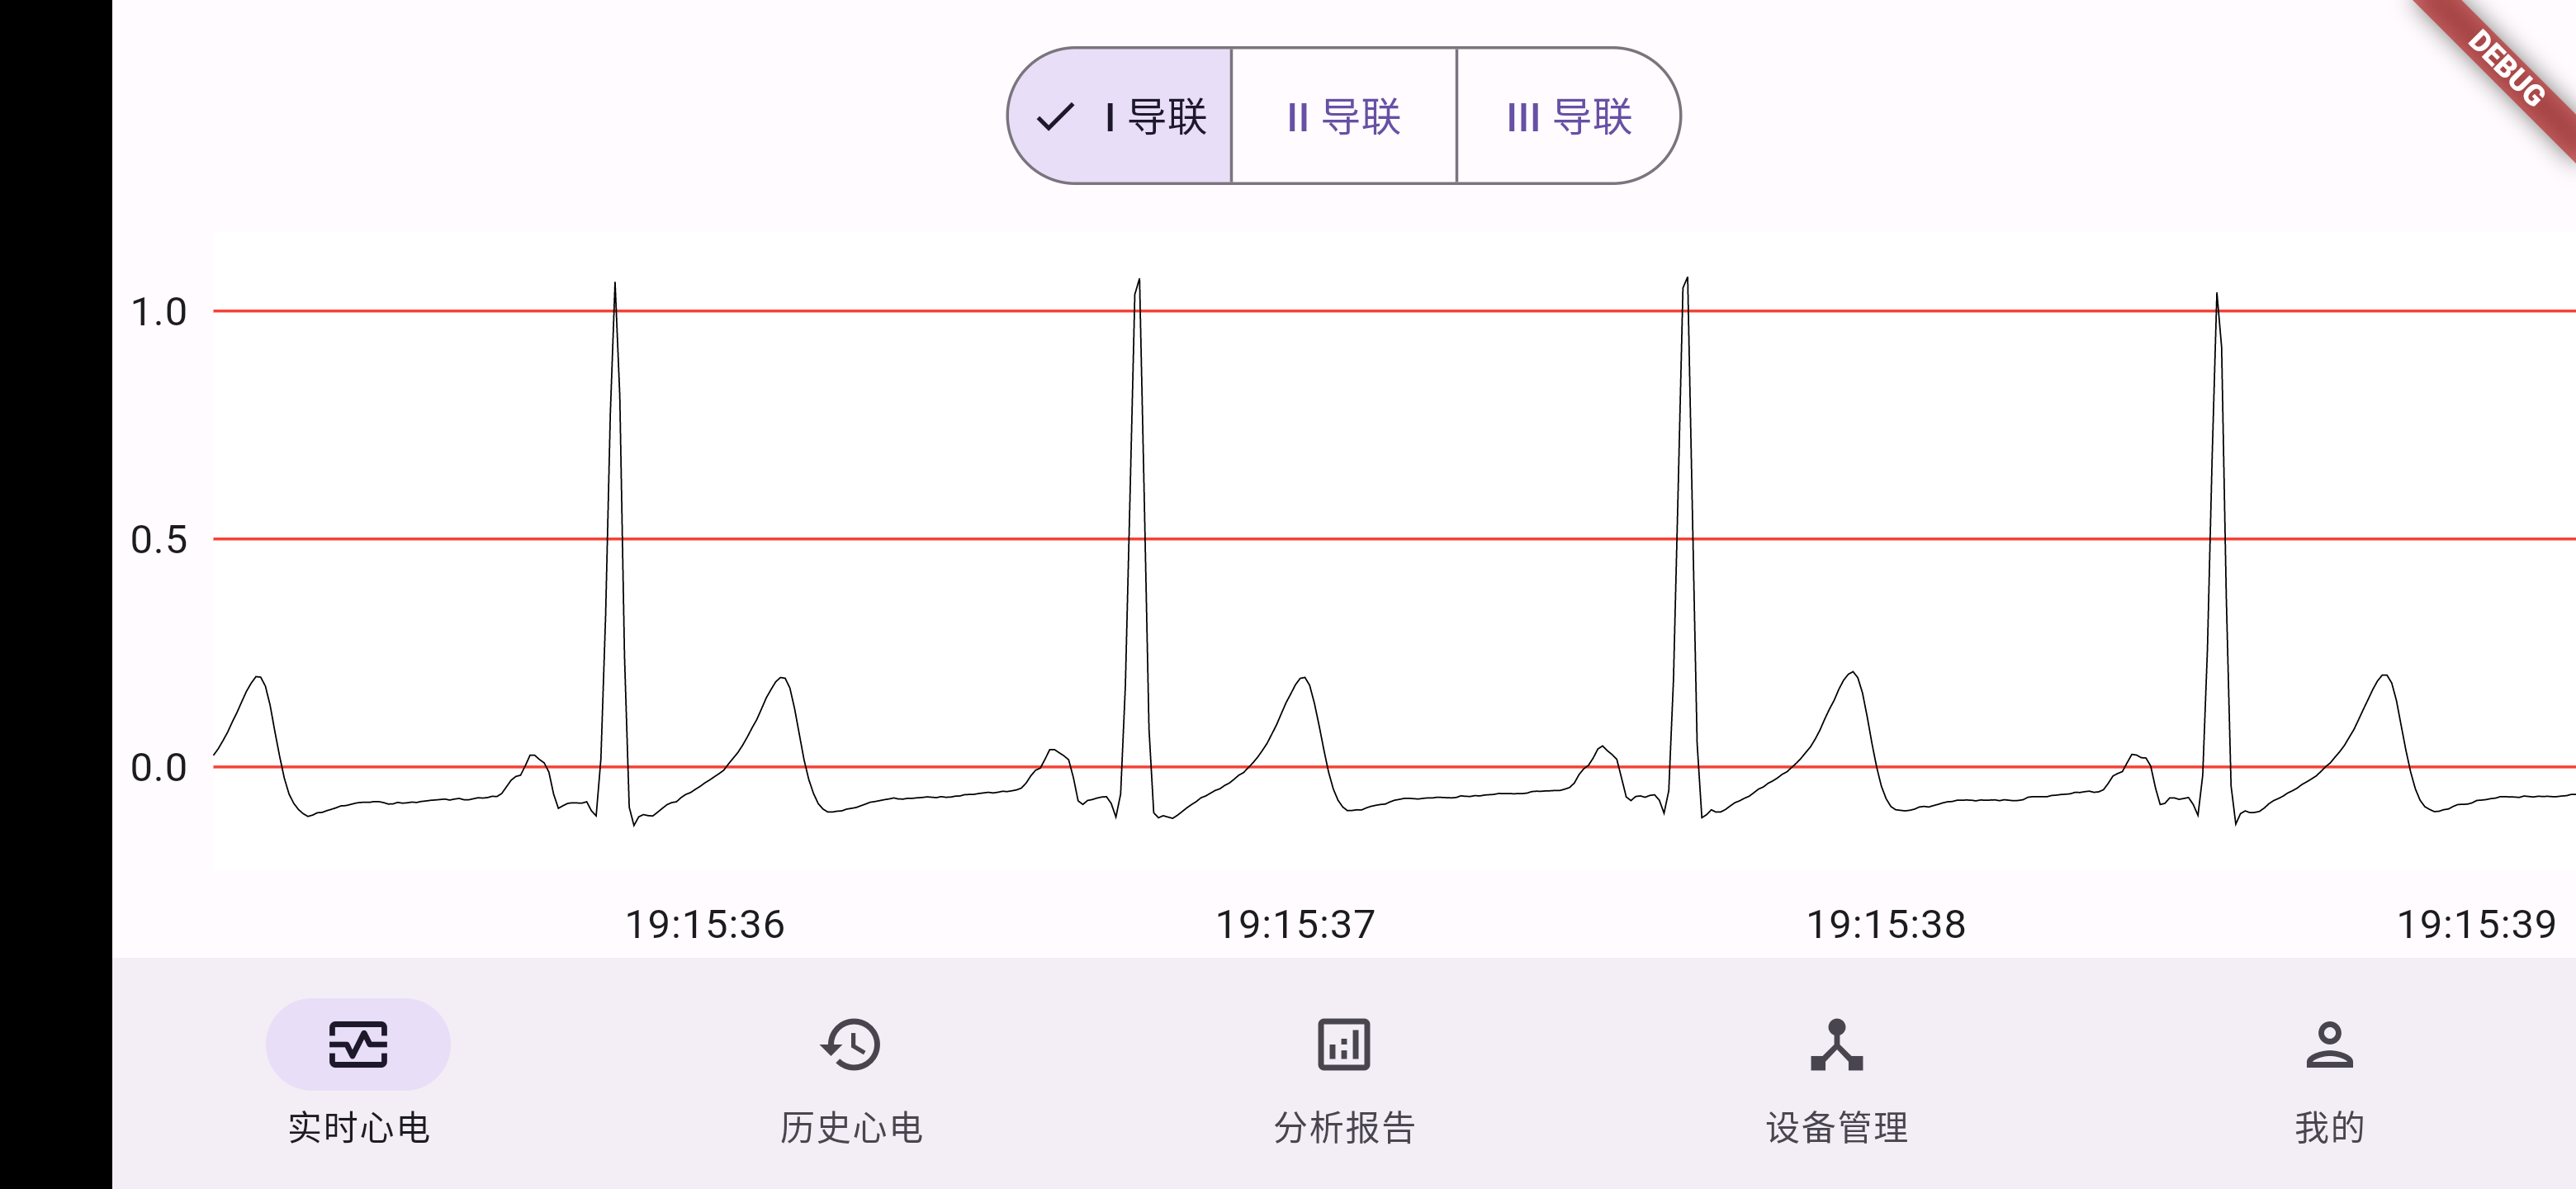
\includegraphics[width=\textwidth]{../assets/real-time-landscape}
    \bicaption{横屏状态下的心电图设计}{Design of the ECG in landscape mode}
    \label{fig:real-time-landscape}
\end{figure}

在横屏状态下,应用会进入全屏状态,隐去系统自带的状态栏等元素。在应用界面内部,顶端的标题栏以及屏幕上部的心率显示区域也会隐藏,以提供更多纵向空间。心电图区域会由同时显示三个导联变为仅显示单个导联,并将心电图上方的导联名称替换为分段按钮,以便用户可以在不同的导联之间进行切换。在横屏状态下,应用在心电图之外仍然为上方的导联切换按钮与下方的导航栏保留了足够的空间。这一方面是因为Material规范要求可点击的元素必须保留足够的大小,以便用户可以轻松点击;另一方面是因为如果要让心电图在保持横纵比例不变的情况下显示更长的时间,纵向空间就需要进行相应缩减;同时,这也保证了在横屏状态下仍然可以正常使用应用的基本功能,使用户不需要在进行切换界面等操作之前先将设备恢复为竖屏状态。

\subsubsection{设备未连接状态的设计}\label{subsubsec:real-time-na-design}

在设备未连接的情况下,由于无从获取实时心电数据,实时心电界面没有可供查看的实际内容。如果仅显示没有数据的空心电图,可能会使用户产生疑惑。因此,在设备未连接的情况下,应用会将实时心电界面替换为一个特殊的错误提示界面。该界面非常简洁,仅在显示区域的中央包含两个元素,竖向排布并留有一定间隔。上方以较大字体显示“设备未连接”的提示信息,下方以按钮形式提供前往设备管理界面的入口,提醒用户检查设备的状态。由于用户可能会在应用保持处于该界面的情况下调试心电设备,所以即使在心电设备尚未连接的情况下,应用也不会自动重定向至设备管理页,而是在用户手动点击按钮后才会跳转。

Material设计提供了各种风格的按钮外观设计。在该提示界面中,比较适用的几种风格如图~\ref{fig:buttons} 所示。

\begin{figure}[ht]
    \subcaptionbox{抬升按钮}{
\includegraphics[width=.196\textwidth]{../assets/button-elevated}}
    \subcaptionbox{填充按钮}{
\includegraphics[width=.196\textwidth]{../assets/button-filled}}
    \subcaptionbox{填充色调按钮}{
\includegraphics[width=.196\textwidth]{../assets/button-filled-tonal}}
    \subcaptionbox{轮廓按钮}{
\includegraphics[width=.196\textwidth]{../assets/button-outlined}}
    \subcaptionbox{文本按钮}{
\includegraphics[width=.196\textwidth]{../assets/button-text}}
    \bicaption{各种风格的按钮对比}{Comparison of different button styles}
    \label{fig:buttons}
\end{figure}

图中从左到右分别为抬升按钮(Elevated button)、填充按钮(Filled button)、填充色调按钮(Filled tonal button)、轮廓按钮(Outlined button)和文本按钮(Text button)。其中,抬升按钮因其阴影效果较易与其他元素之间产生不协调感,被规定为仅在绝对必要的时候,比如需要从图案背景中进行视觉分离时等特殊情况下才应使用,显然此界面并不属于应添加阴影的特殊情况。其余四种按钮的强调程度由强至弱,应当按需使用。由于该界面元素较少,所以不需要对该按钮进行较为强烈的强调,故未使用两种填充按钮。如果使用文本按钮,则视觉效果过于微弱,甚至使用户有些难以察觉到这是一个按钮。最终,选定了轮廓按钮的风格,其强调程度充足但不过度,与其他元素最为协调。

\subsubsection{应用中图标的设计}\label{subsubsec:icons}

实时心电界面在导航栏中的图标使用了常见的心电图的标志,这是根据该界面的主要内容决定的。

Material规范对于图标的设计与使用有一些相关要求。本应用为了遵循规范,使用的均是Google官方提供的图标。Google为其图标提供了各种风格的样式,常见的几种如图~\ref{fig:icons} 所示。

\begin{figure}[ht]
    \centering
    \subcaptionbox{轮廓}{
\includegraphics[width=.15\textwidth]{../assets/icon-outlined}}
    \subcaptionbox{圆润}{
\includegraphics[width=.15\textwidth]{../assets/icon-rounded}}
    \subcaptionbox{尖锐}{
\includegraphics[width=.15\textwidth]{../assets/icon-sharp}}
    \subcaptionbox{常规(旧)}{
\includegraphics[width=.15\textwidth]{../assets/icon-old-outlined}}
    \subcaptionbox{填充(旧)}{
\includegraphics[width=.15\textwidth]{../assets/icon-old-filled}}
    \bicaption{Material图标的各种风格}{Different styles of Material icons}
    \label{fig:icons}
\end{figure}

图中的前三种风格是Material 3新增的,通常应该比旧版优先使用。具体使用哪一种风格应该根据应用程序的整体设计风格来确定,比如圆润的图标使用了较多圆角,与使用较重的排版、弯曲徽标或圆形元素来表达其风格的品牌搭配得很好;尖锐的图标则带有较多直角,体现出清晰锐利的风格。本应用内的所有图标都使用了轮廓风格,这和整个应用的轻盈、干净的设计风格保持一致。

\subsection{历史心电界面的设计}\label{subsec:history-design}

历史心电界面的整体设计如图~\ref{fig:history} 所示。

\begin{figure}[ht]
    \subcaptionbox{加载中}{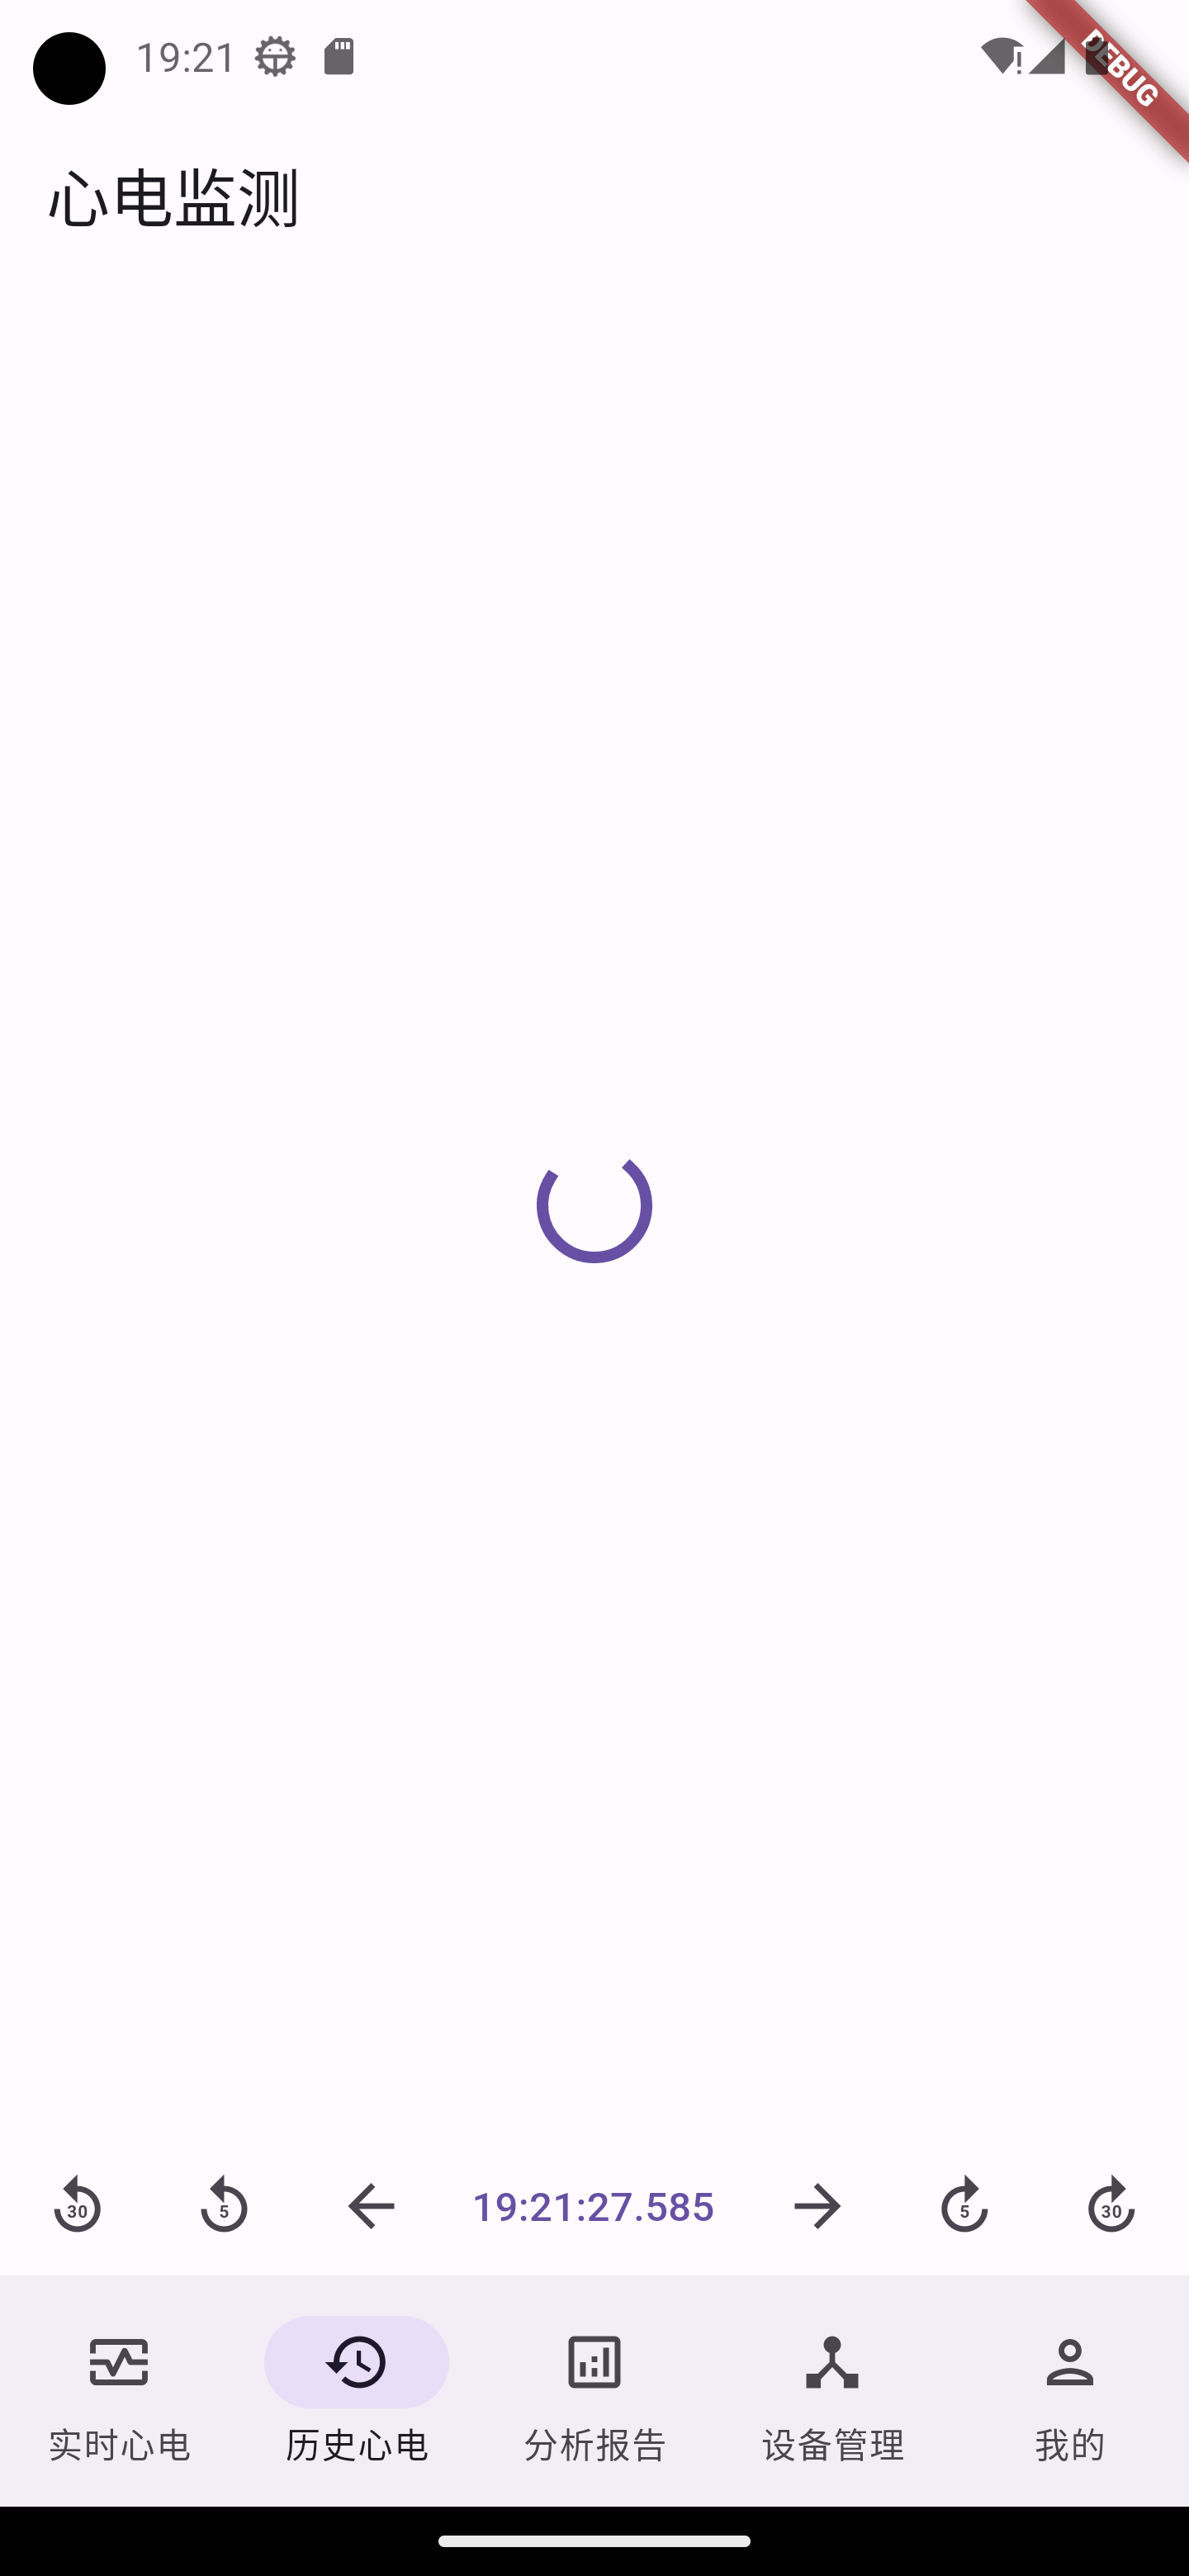
\includegraphics[width=.33\textwidth]{../assets/history-loading}}
    \subcaptionbox{正常状态}{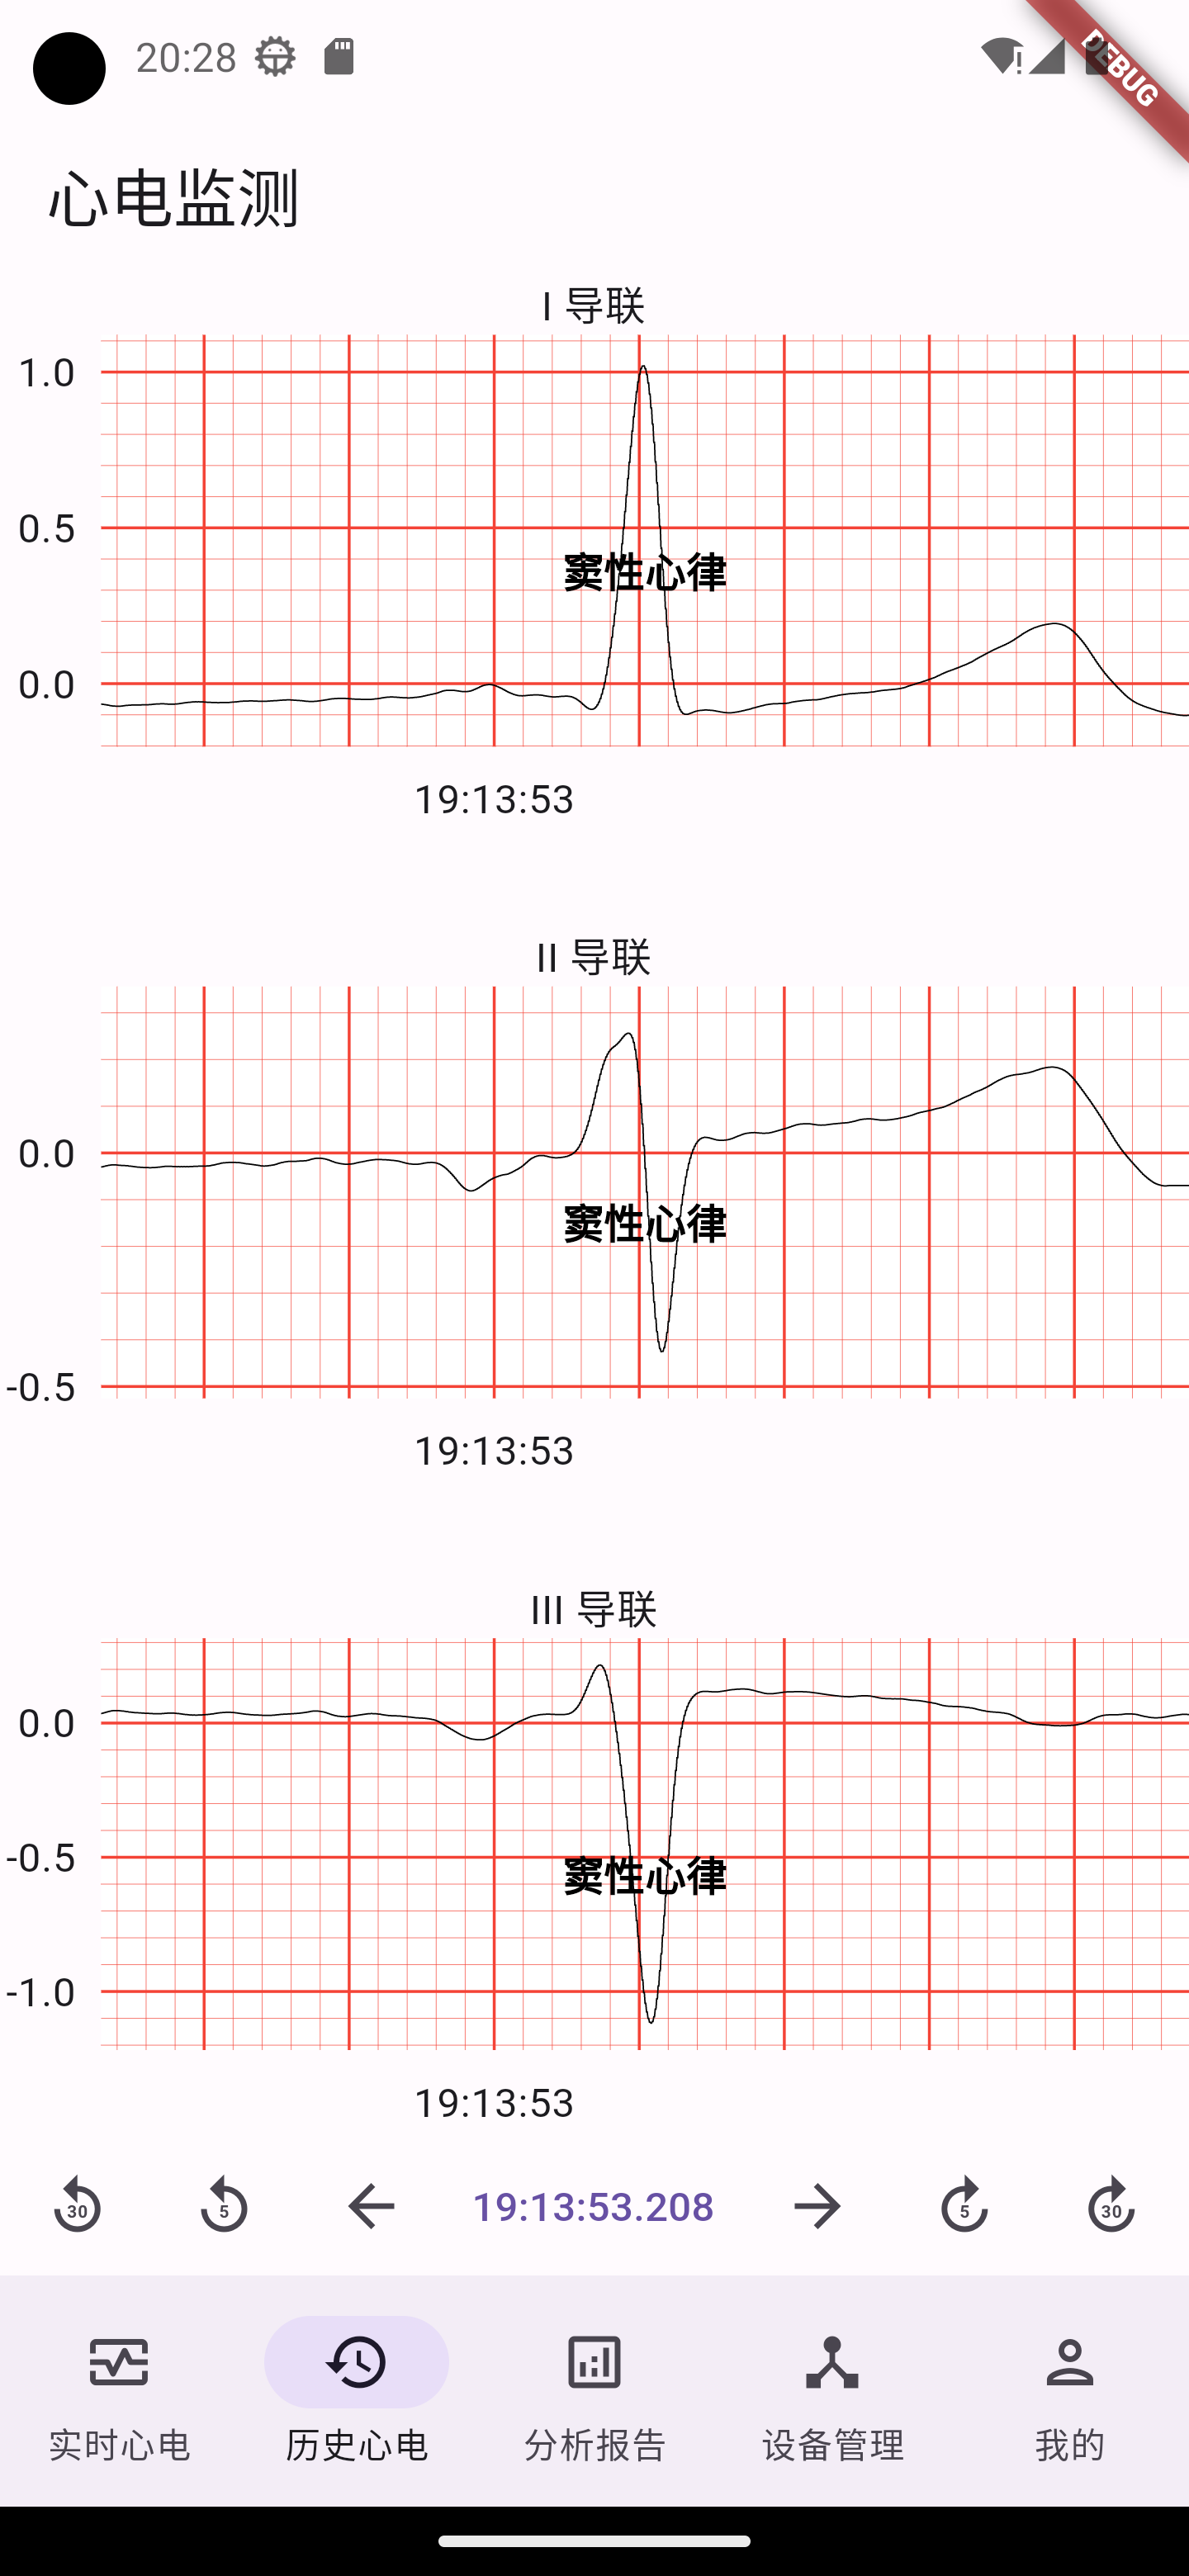
\includegraphics[width=.33\textwidth]{../assets/history}}
    \subcaptionbox{无数据}{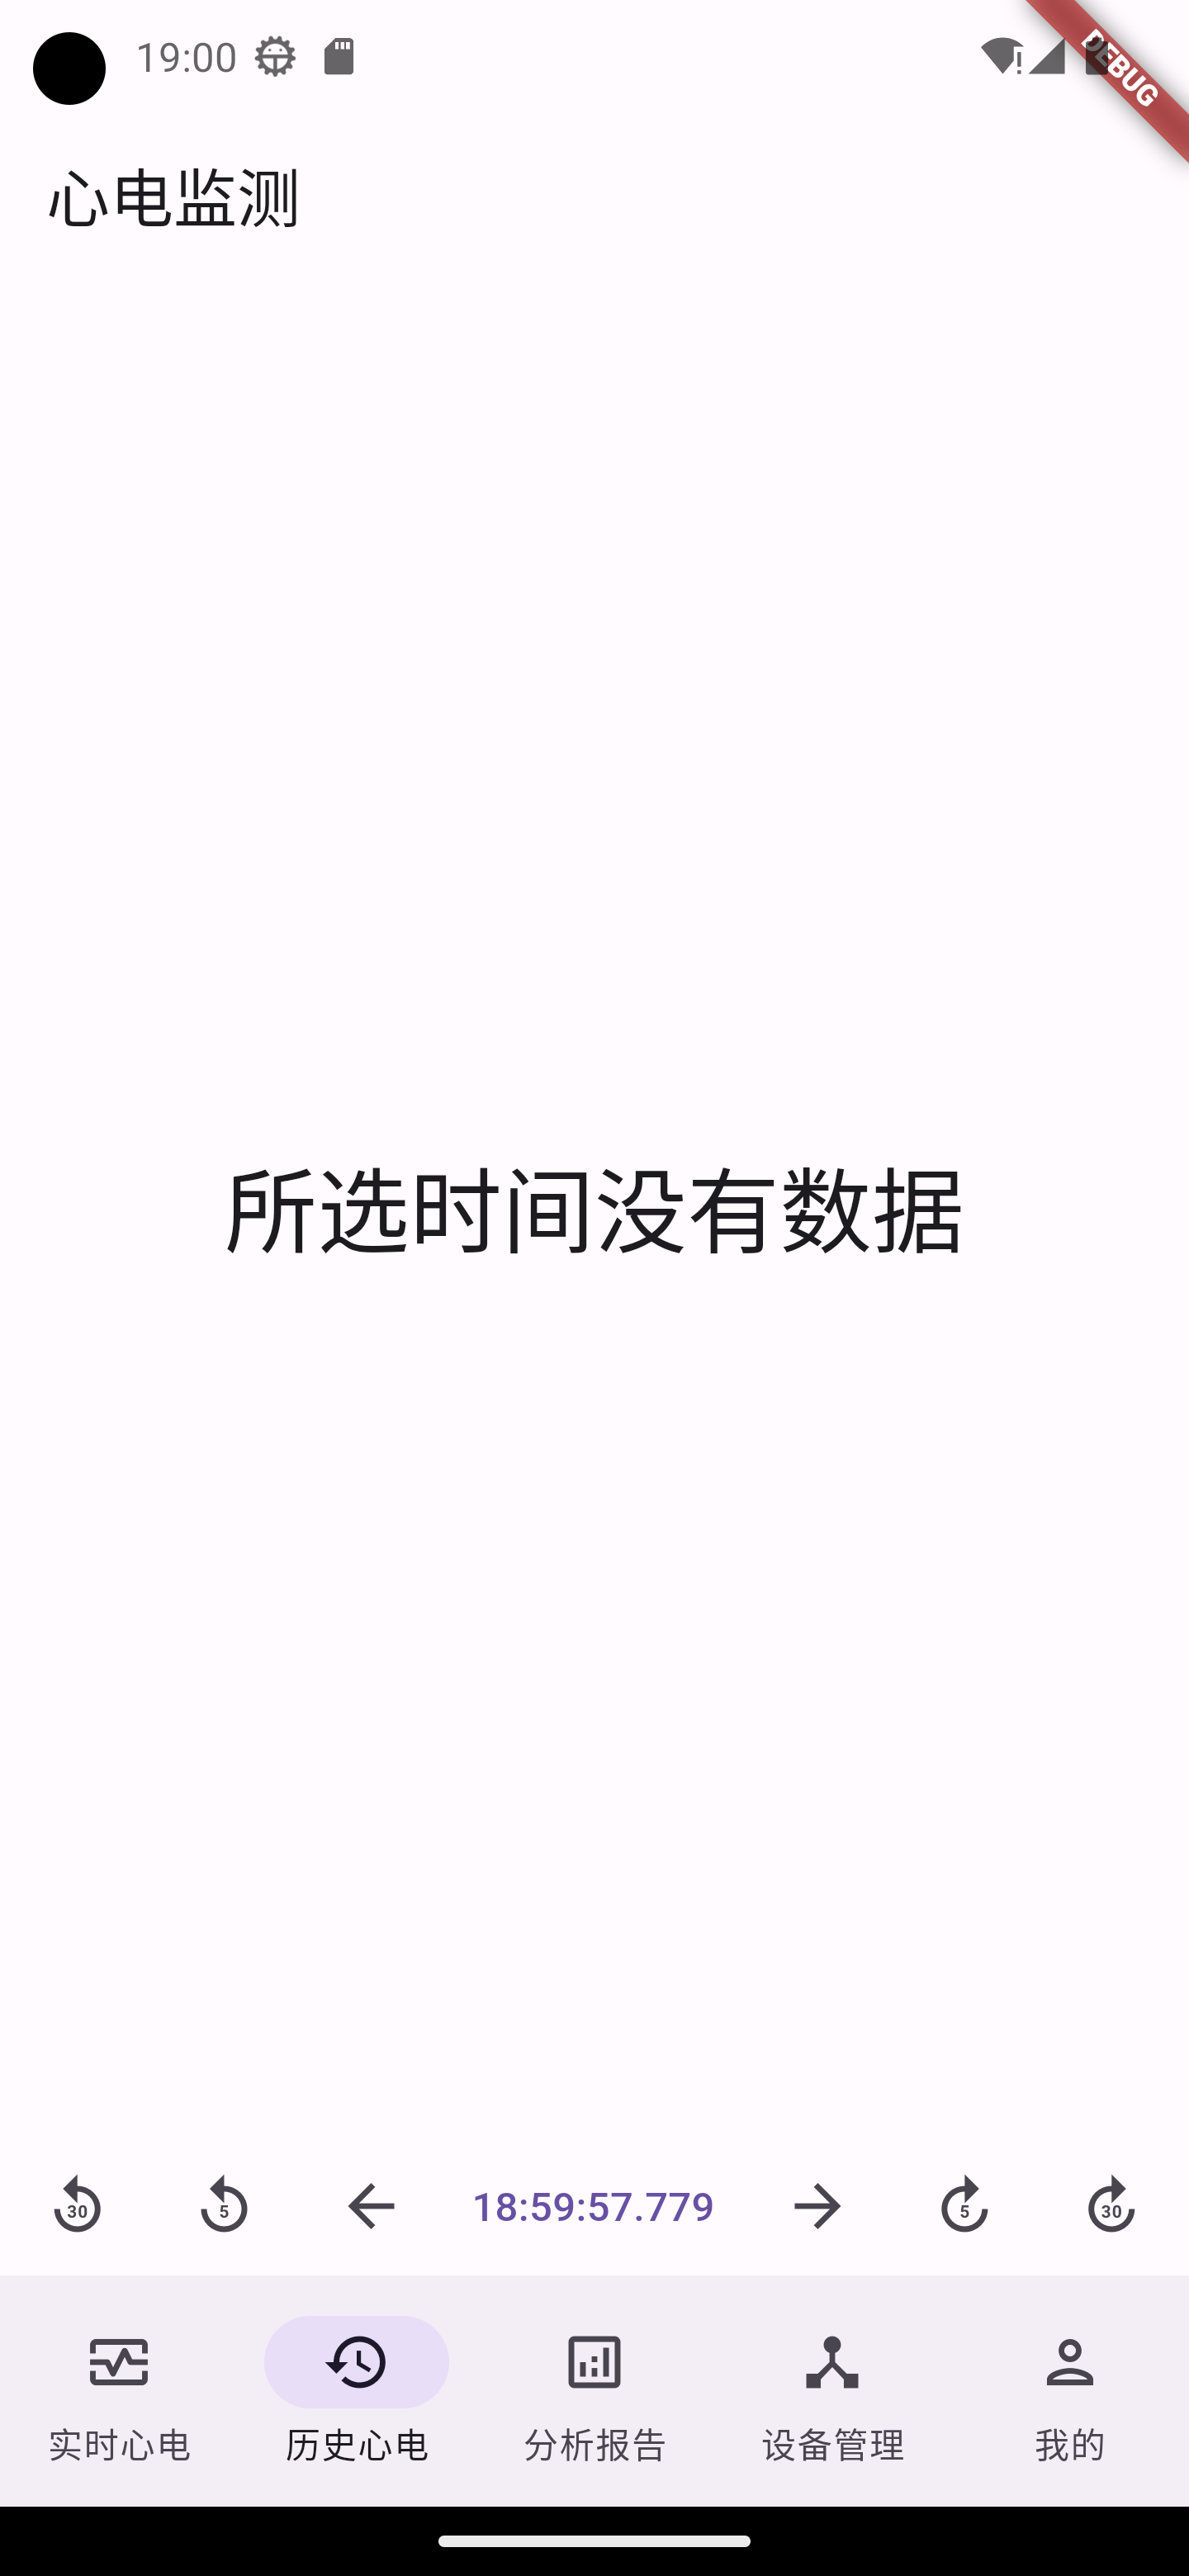
\includegraphics[width=.33\textwidth]{../assets/history-na}}
    \bicaption{历史心电界面的设计}{Design of the history ECG page}
    \label{fig:history}
\end{figure}

该界面由两部分组成,分别是上方的心电图部分和下方的时间选择器部分。为了与实时心电进行区分,导航栏中的图标使用了表示历史记录的符号。

\subsubsection{心电图部分的设计}\label{subsubsec:history-ecg-design}

历史心电图与实时心电图的总体设计相同,重复部分不须赘述。相比实时心电图,历史心电图因其性质而在设计上具有一些不同点。

首先,关于心电图背景的网格,在实时心电图中完全隐去了纵线、部分显示了横线,如上文所述是因为心电图在不停横向移动。但是在历史心电图中,图中显示的数据是静态的,在用户不调整所选时间的情况下不会发生变动。因此,没有必要在历史心电图中隐去或部分隐去背景的坐标网格。在历史心电图的设计中,背景的网格线与实际的心电图纸保持一致,以粗线分割大格,每大格里再以细线(实际显示为颜色较浅的线)分割为5小格。这样的设计可以使得心电图上各点的数值更加清晰,方便用户对历史心电数据进行仔细查看。

另一个显著的不同点在于历史心电图中对每个心拍的类型进行了标注。由于所使用的智能检测算法是离线算法,无法实时给出心拍类型,因此该标注在实时心电图中无法实现,仅可在历史心电图中进行查看。心拍的类型以文本形式直接显示在每个导联的心电图中对应位置的中央。一个被考虑过的替代方案是在R波(心电图中幅度最大的波)的波峰所在的点进行标注,但这需要心电图中在上方保留一些额外的空间,不太适合移动设备的较小的屏幕,而且各个导联中的波峰也并非完全同步。另一个可能的替代方案是使用颜色而非文本对心拍类型进行标注,但这种方案要么需要在屏幕上的某处显示各种颜色对应的标签而不适合小屏幕设备,要么需要用户在某个说明界面中查看并记忆各种标签的颜色而严重影响了应用的易用性,因此也没有采用。

此外,该部分区域存在两种特殊状态,分别是加载中和无数据的状态。经过对数据库的优化之后,加载中状态持续的时间很短,仅在设备性能较差、数据库索引未完成、缓存也未命中等情况同时发生的状态下才会有较长时间的加载;因此,加载中界面仅简单使用了一个圆形的不确定进度的加载动画来指示应用并未失去响应。无数据的状态则是在用户选择的时间前后内没有心电数据的情况下出现的,可能是由于用户在该时间并未佩戴监测设备,或是应用后台进程因各种原因被终止而缺失该时间的数据,也可能是用户刚刚开始使用该应用但试图查询几小时前的数据。在没有可用数据的情况下,该区域并不会显示只有背景的空心电图,而是会直接显示所选时间没有数据的提示。

\subsubsection{时间选择器部分的设计}\label{subsubsec:history-time-picker-design}

时间选择器部分由7个横向排开的按钮组成,按钮之间等间距,左右两侧不留额外空间。由于按钮在外观和功能上都采用了左右对称的设计,因此只对左起的4个按钮进行说明。

前两个按钮分别使用了在倒退符号中包含数字30和数字5的图标,按钮功能分别为将所选时间调整为30秒前和5秒前。

第三个按钮使用了向左的箭头作为图标,其作用在不同情况下有所差别。当用户点击该按钮后,如果当前时间之前可以找到另一个心拍,则会跳转至该心拍所在的时间;如果当前时间之前已经没有心拍,比如当前时间所示的是记录内的第一个心拍,或者用户手动跳转到了有数据记录之前的区域,或者算法在数据边界出现了偶然的故障而没有正确识别出心拍,则会跳转到1秒之前,保证该按钮无论如何都不会毫无作用。

第四个按钮,即中间的按钮,其作用相较前几个按钮更多。首先,该按钮作为文本按钮,起到了普通文本的显示作用。其指示的当前查询时间是心电图正中间的时间,并且在切换横竖屏状态时仍然保持该时间在正中间。由于时间选择器的上一个与下一个心拍按钮以及分析报告中跳转心拍所在时间的设计,位于图像中间的通常刚好是某个心拍的R波,这保证了视觉效果最明显的R波恰好会位于用户视觉焦点上。其次,该按钮也提供了相比其他几个按钮更大粒度的时间跳转。点击按钮后,会弹出如图~\ref{fig:history-time-picker} 所示的Material风格的时间选择器,用户可以在其中以表盘模式或数字模式输入要跳转到的时间,点击确定后,时间选择器会自动关闭并将历史心电图跳转至所选时间。由于该自由跳转功能的使用频率远低于其他几个按钮,所以只使用了强调效果最弱的文本按钮,以避免不必要地干扰用户的注意力。

\begin{figure}[ht]
    \centering
    \subcaptionbox{表盘模式输入}{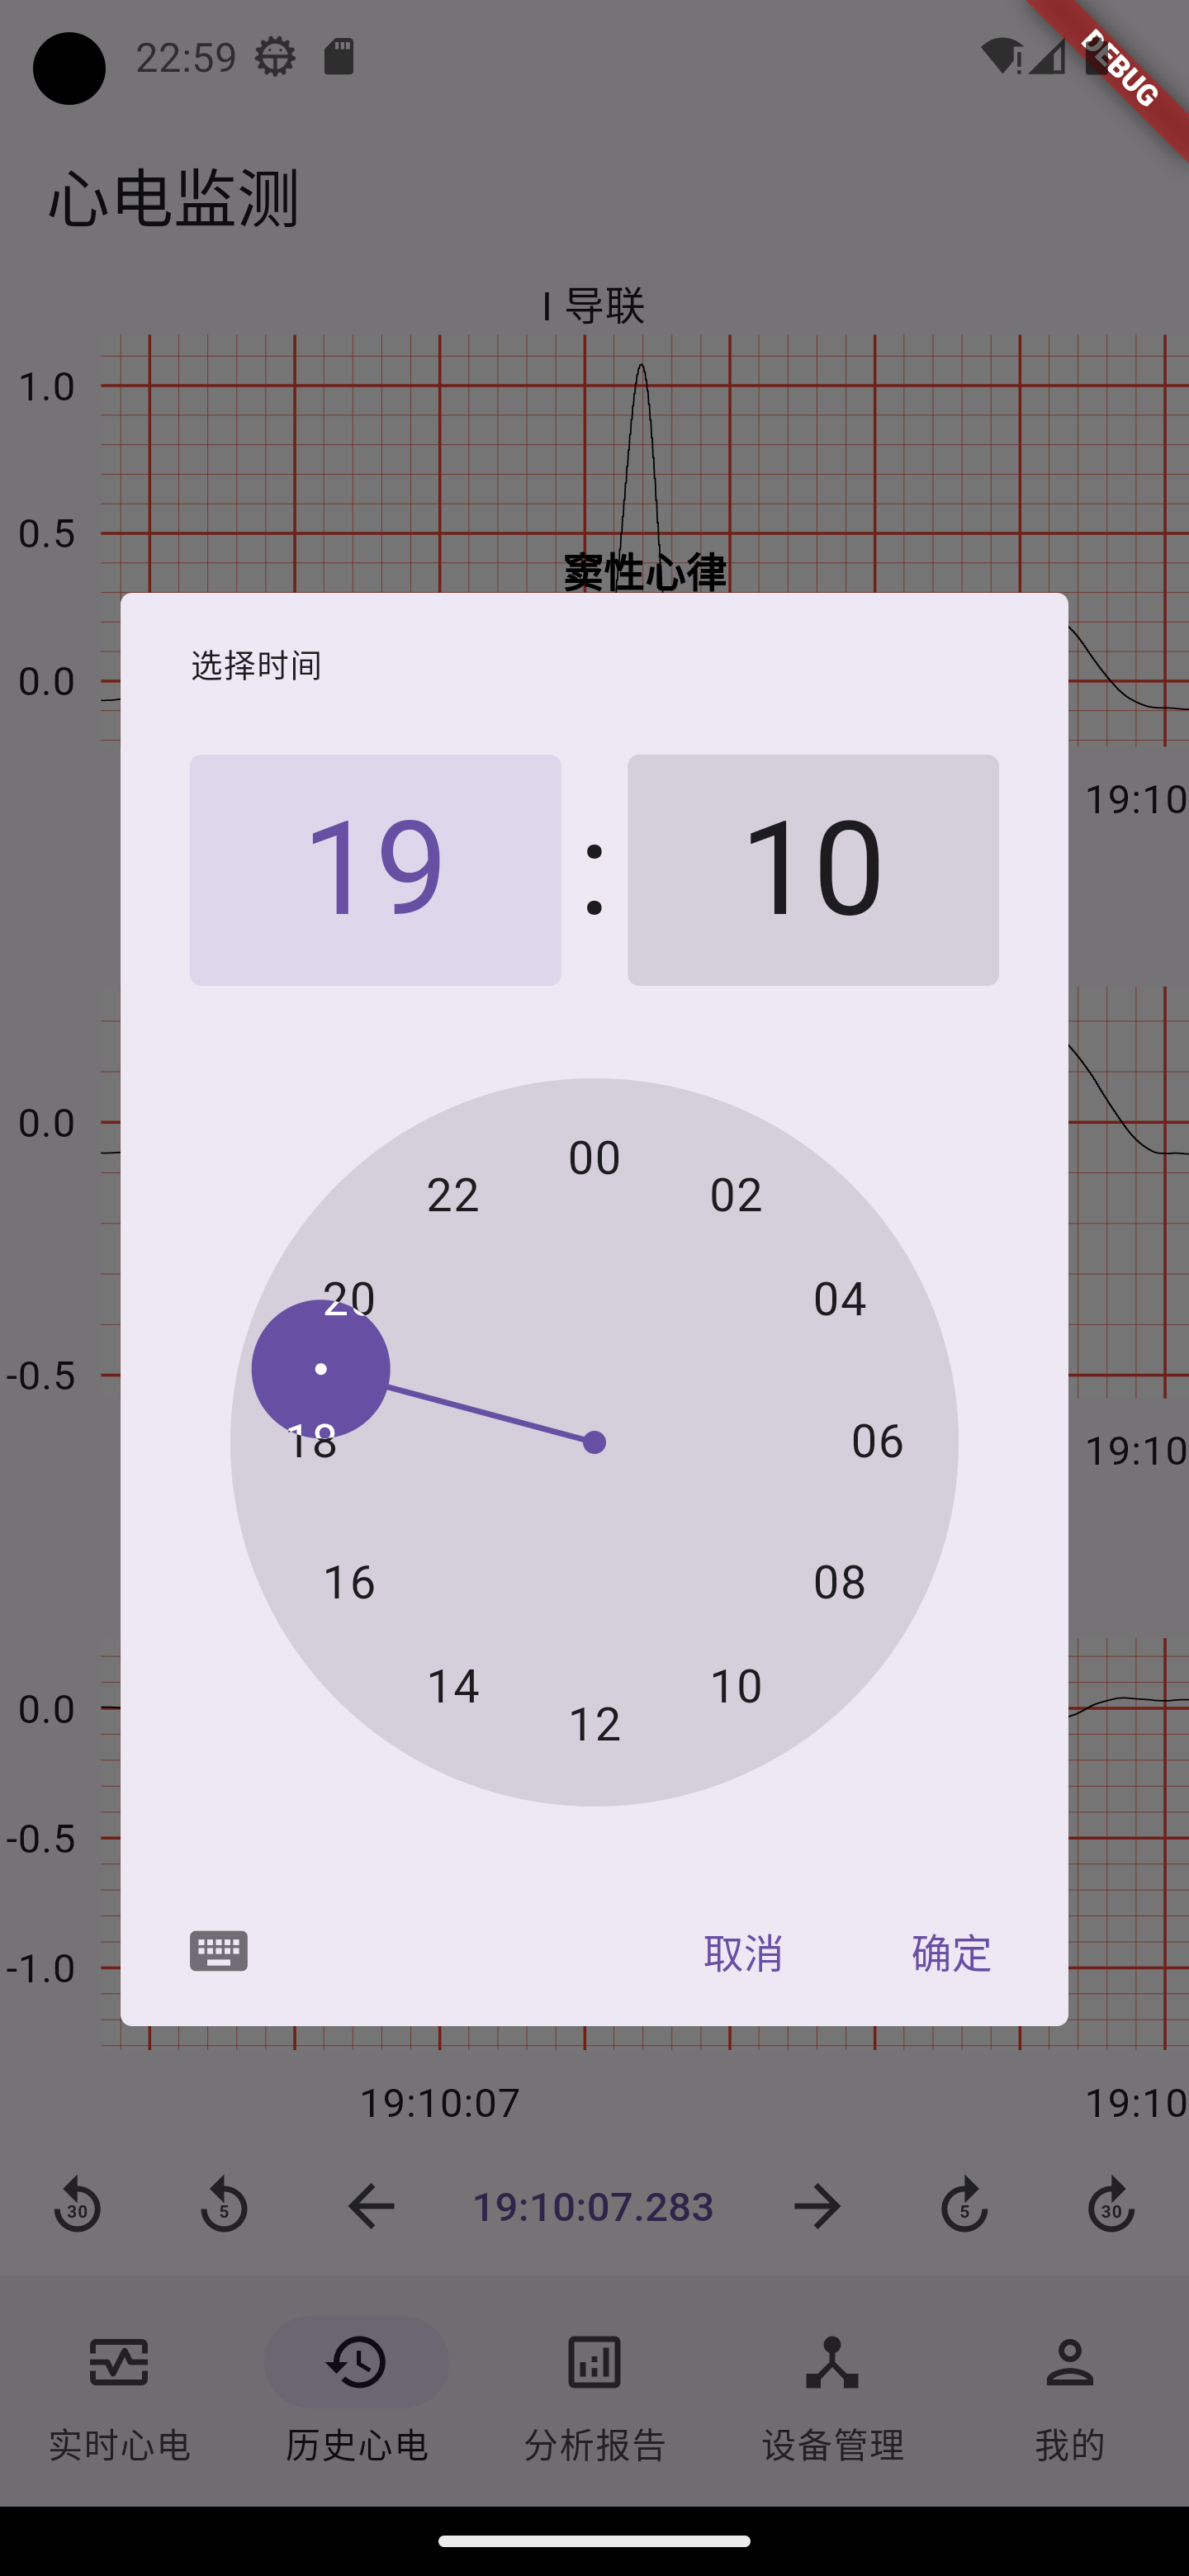
\includegraphics[width=.33\textwidth]{../assets/history-dialog-clock}}
    \subcaptionbox{数字模式输入}{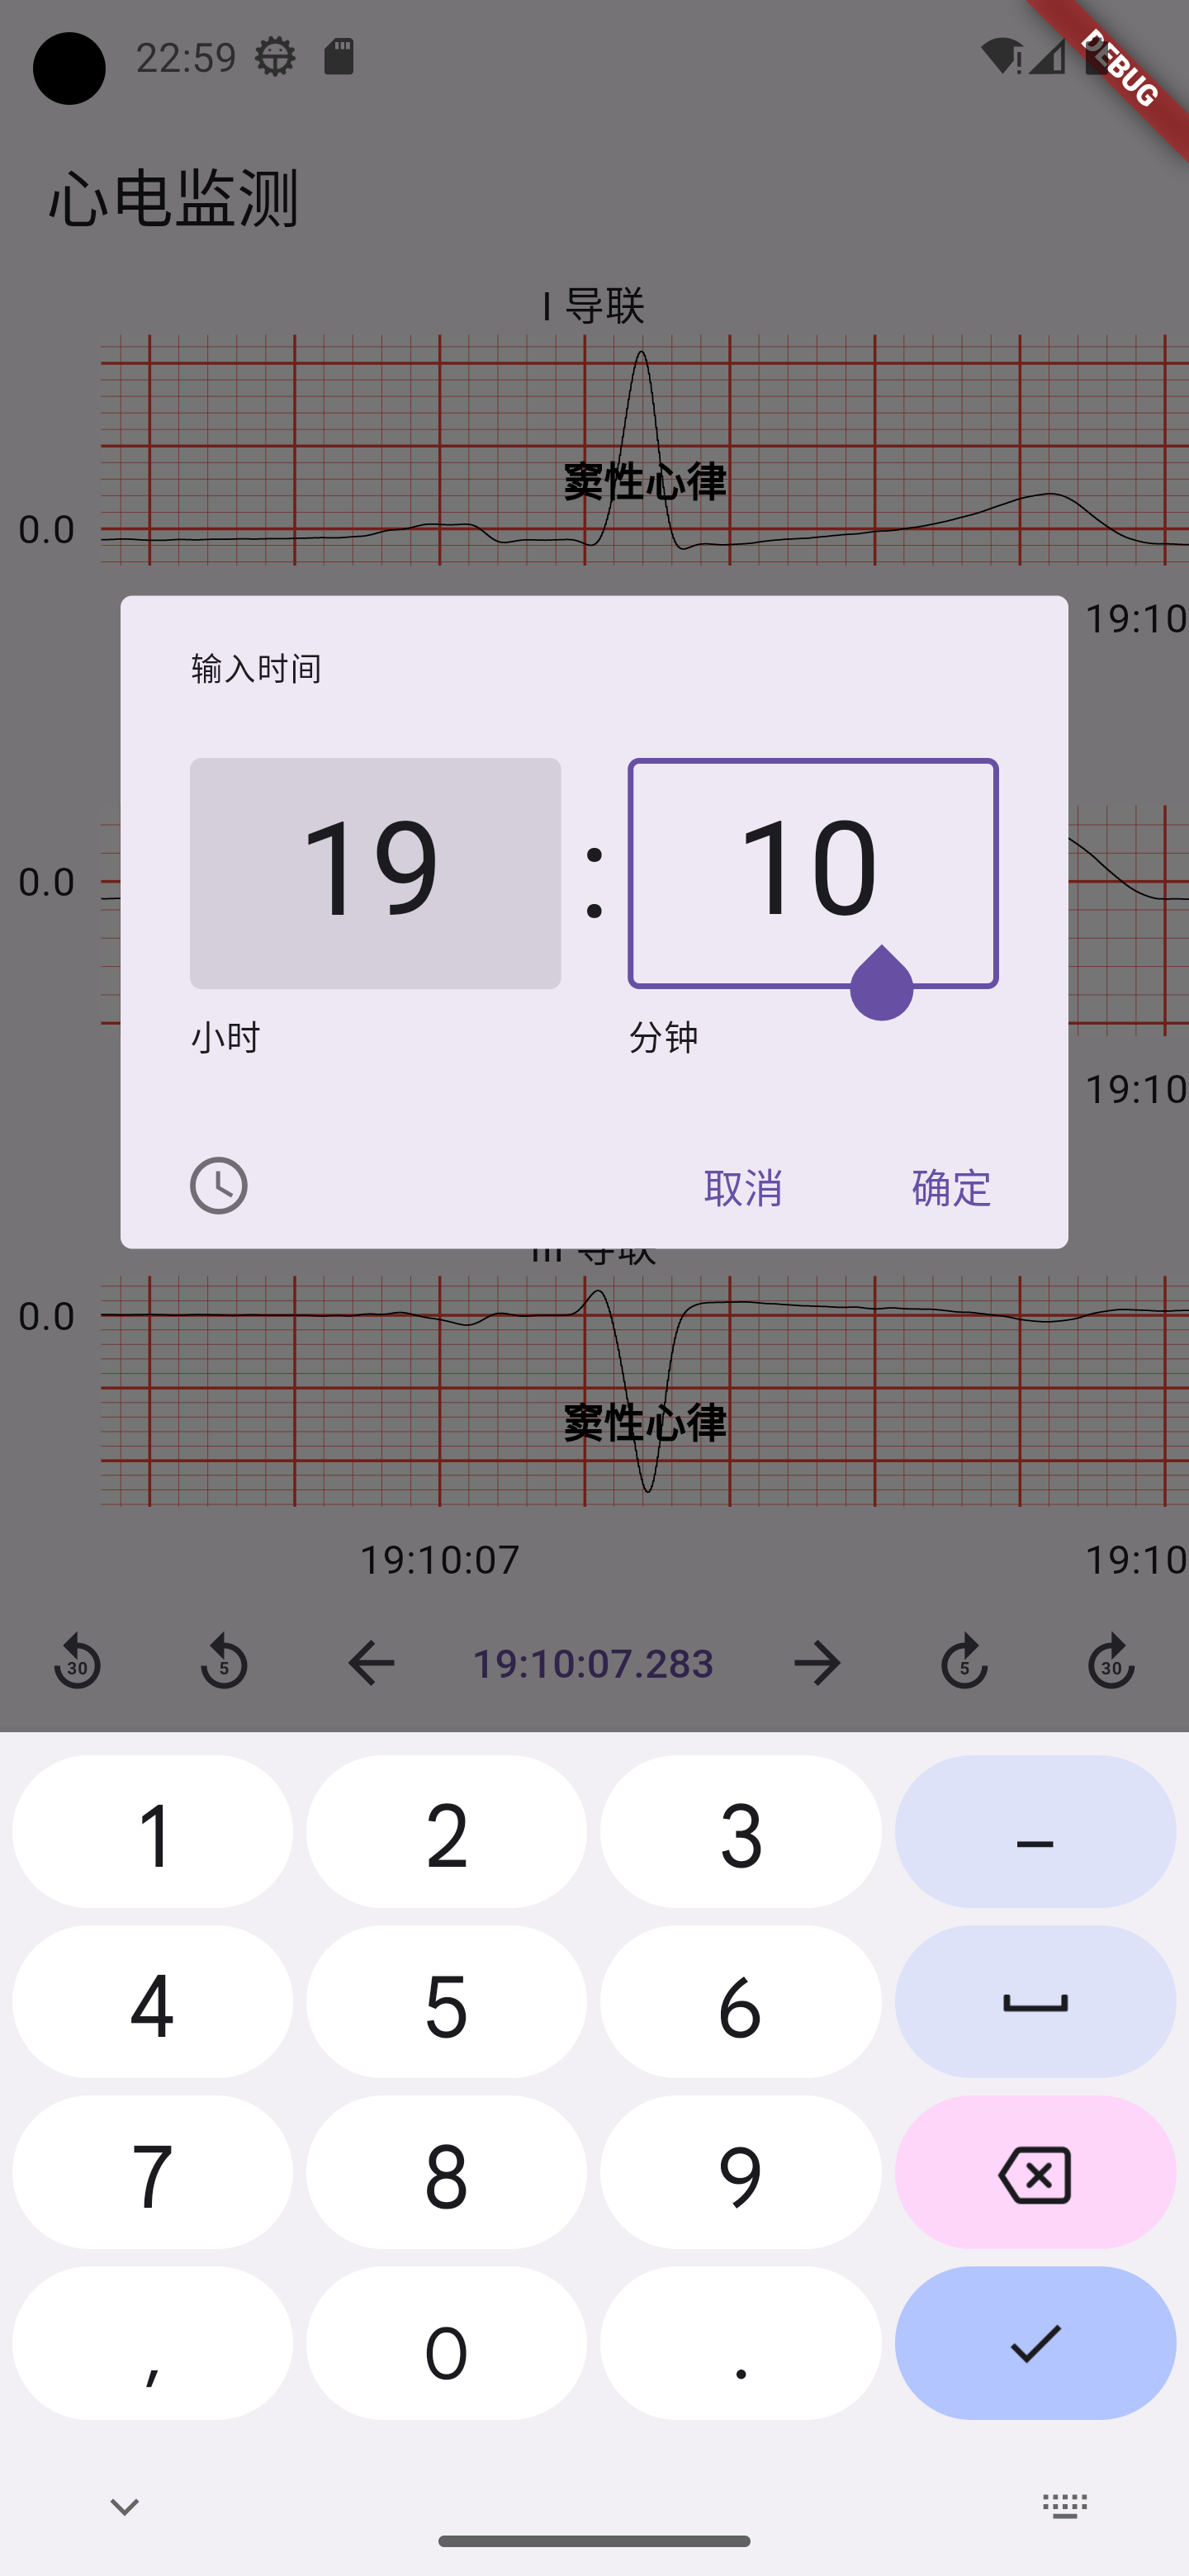
\includegraphics[width=.33\textwidth]{../assets/history-dialog-field}}
    \bicaption{历史心电时间选择器的设计}{Design of the history ECG time picker}
    \label{fig:history-time-picker}
\end{figure}

从图中也可以看出,当可用显示区域由于键盘的弹出而缩小时,应用的界面布局仍然可以保持基本可用。这也体现了应用的设计可以适应不同尺寸、不同屏幕比例的设备,并且对分屏等比例特殊的情况也有支持。

\subsection{分析报告界面的设计}\label{subsec:analytics-design}

分析报告界面的整体设计如图~\ref{fig:analytics} 所示。在导航栏中为分析报告使用了表示数据分析的图标。

\begin{figure}[ht]
    \subcaptionbox{加载中}{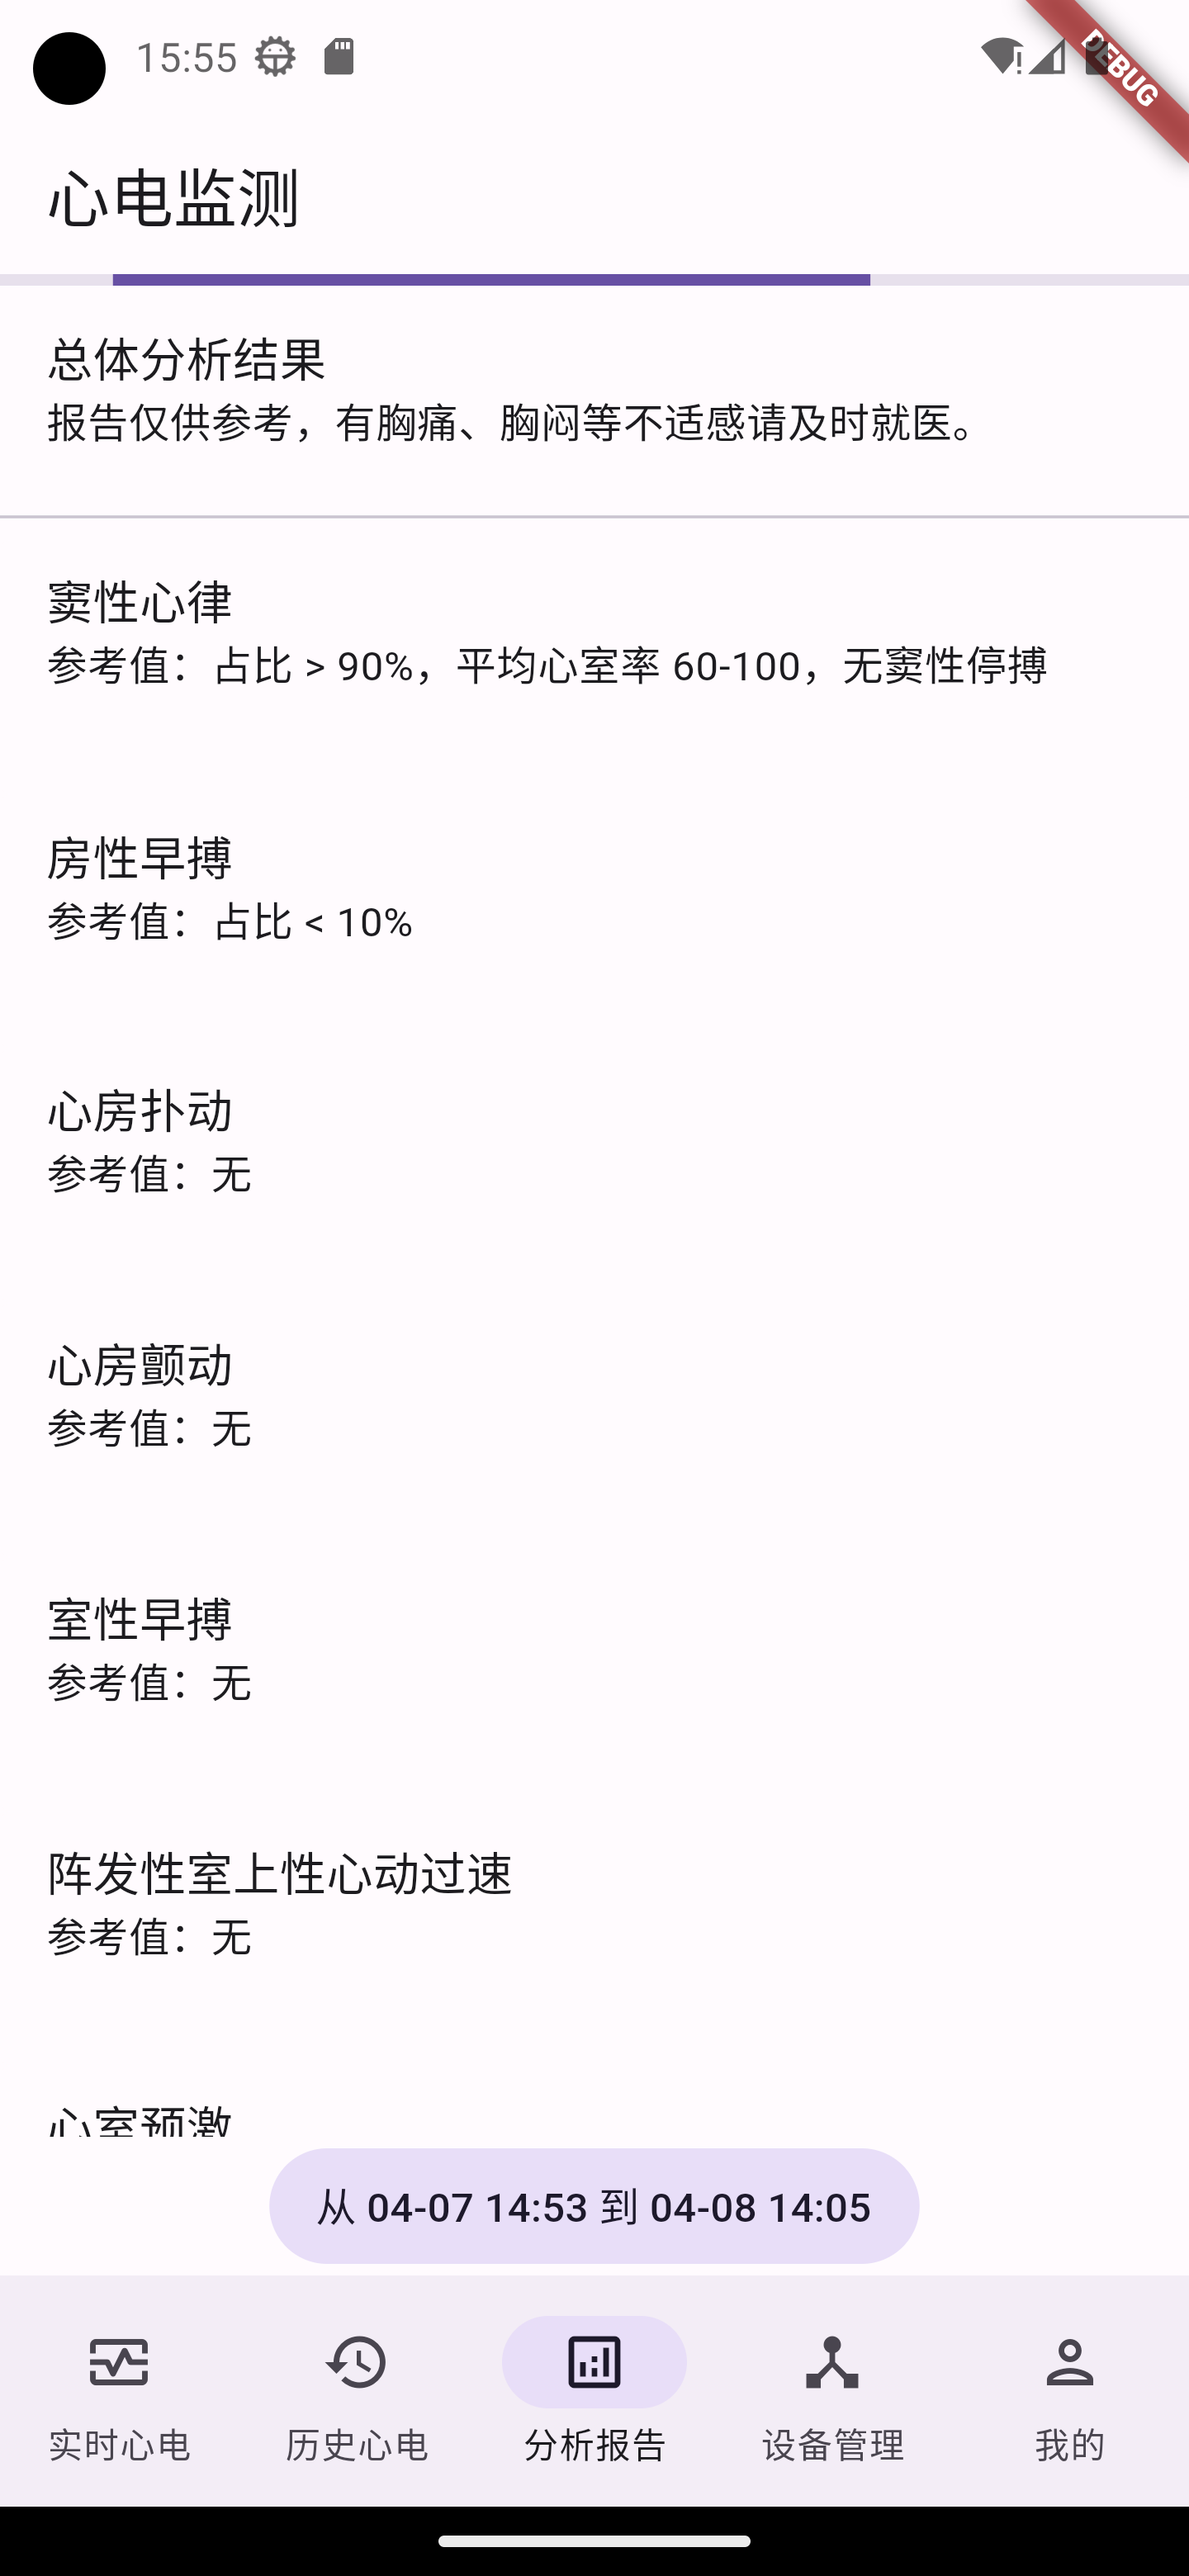
\includegraphics[width=.33\textwidth]{../assets/analytics-loading}}
    \subcaptionbox{正常状态}{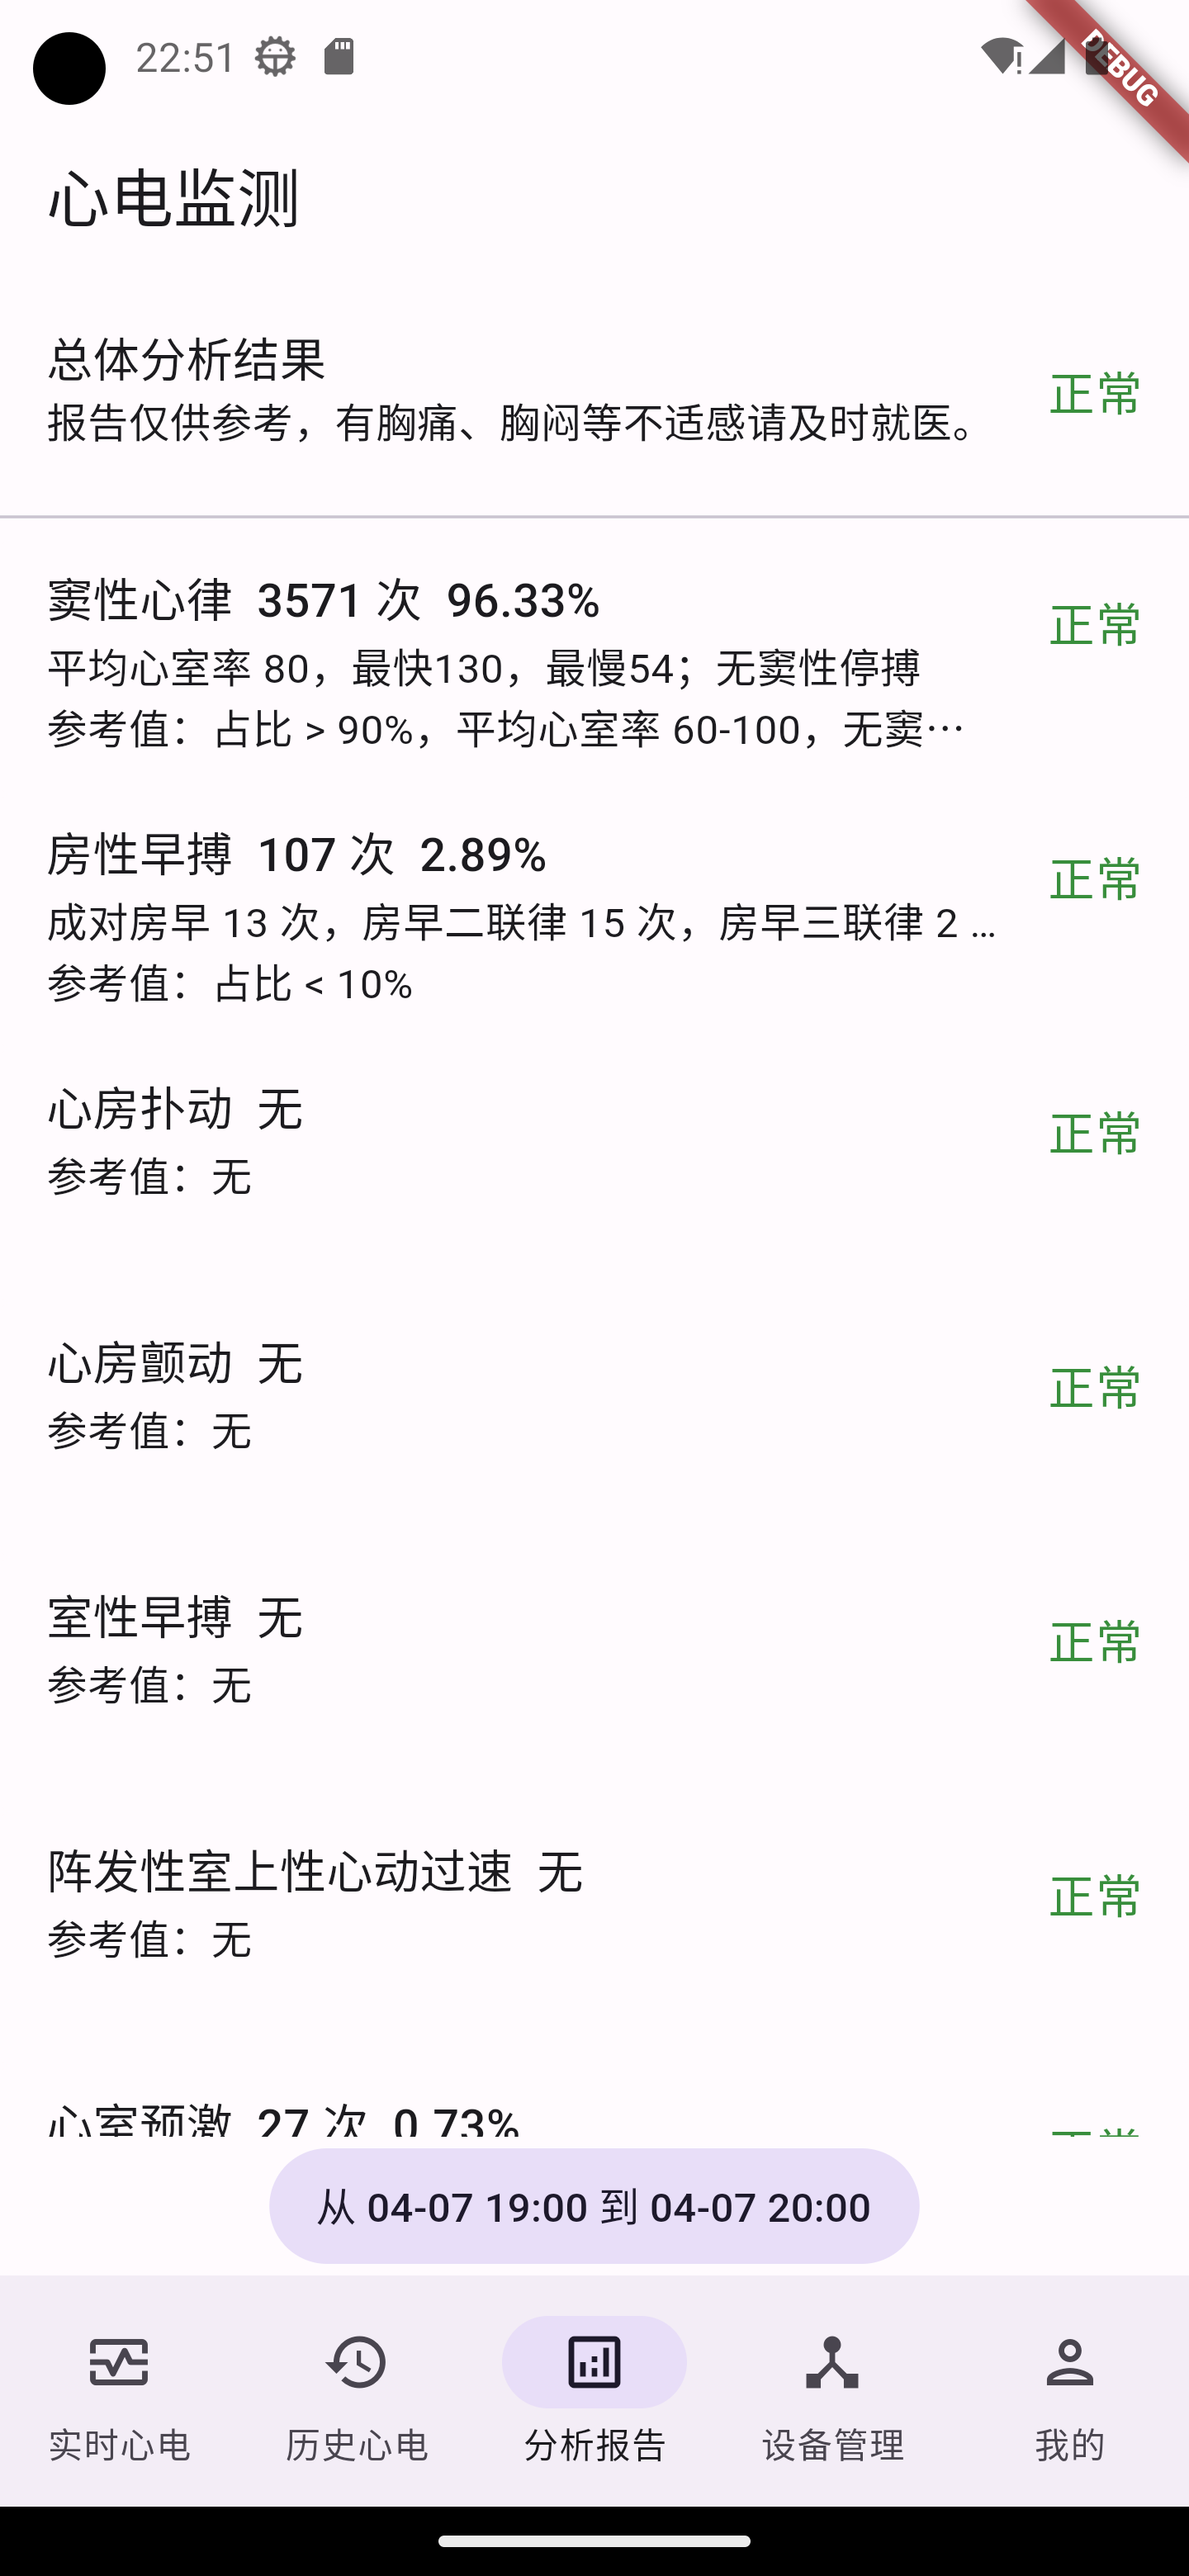
\includegraphics[width=.33\textwidth]{../assets/analytics}}
    \subcaptionbox{时间范围选择}{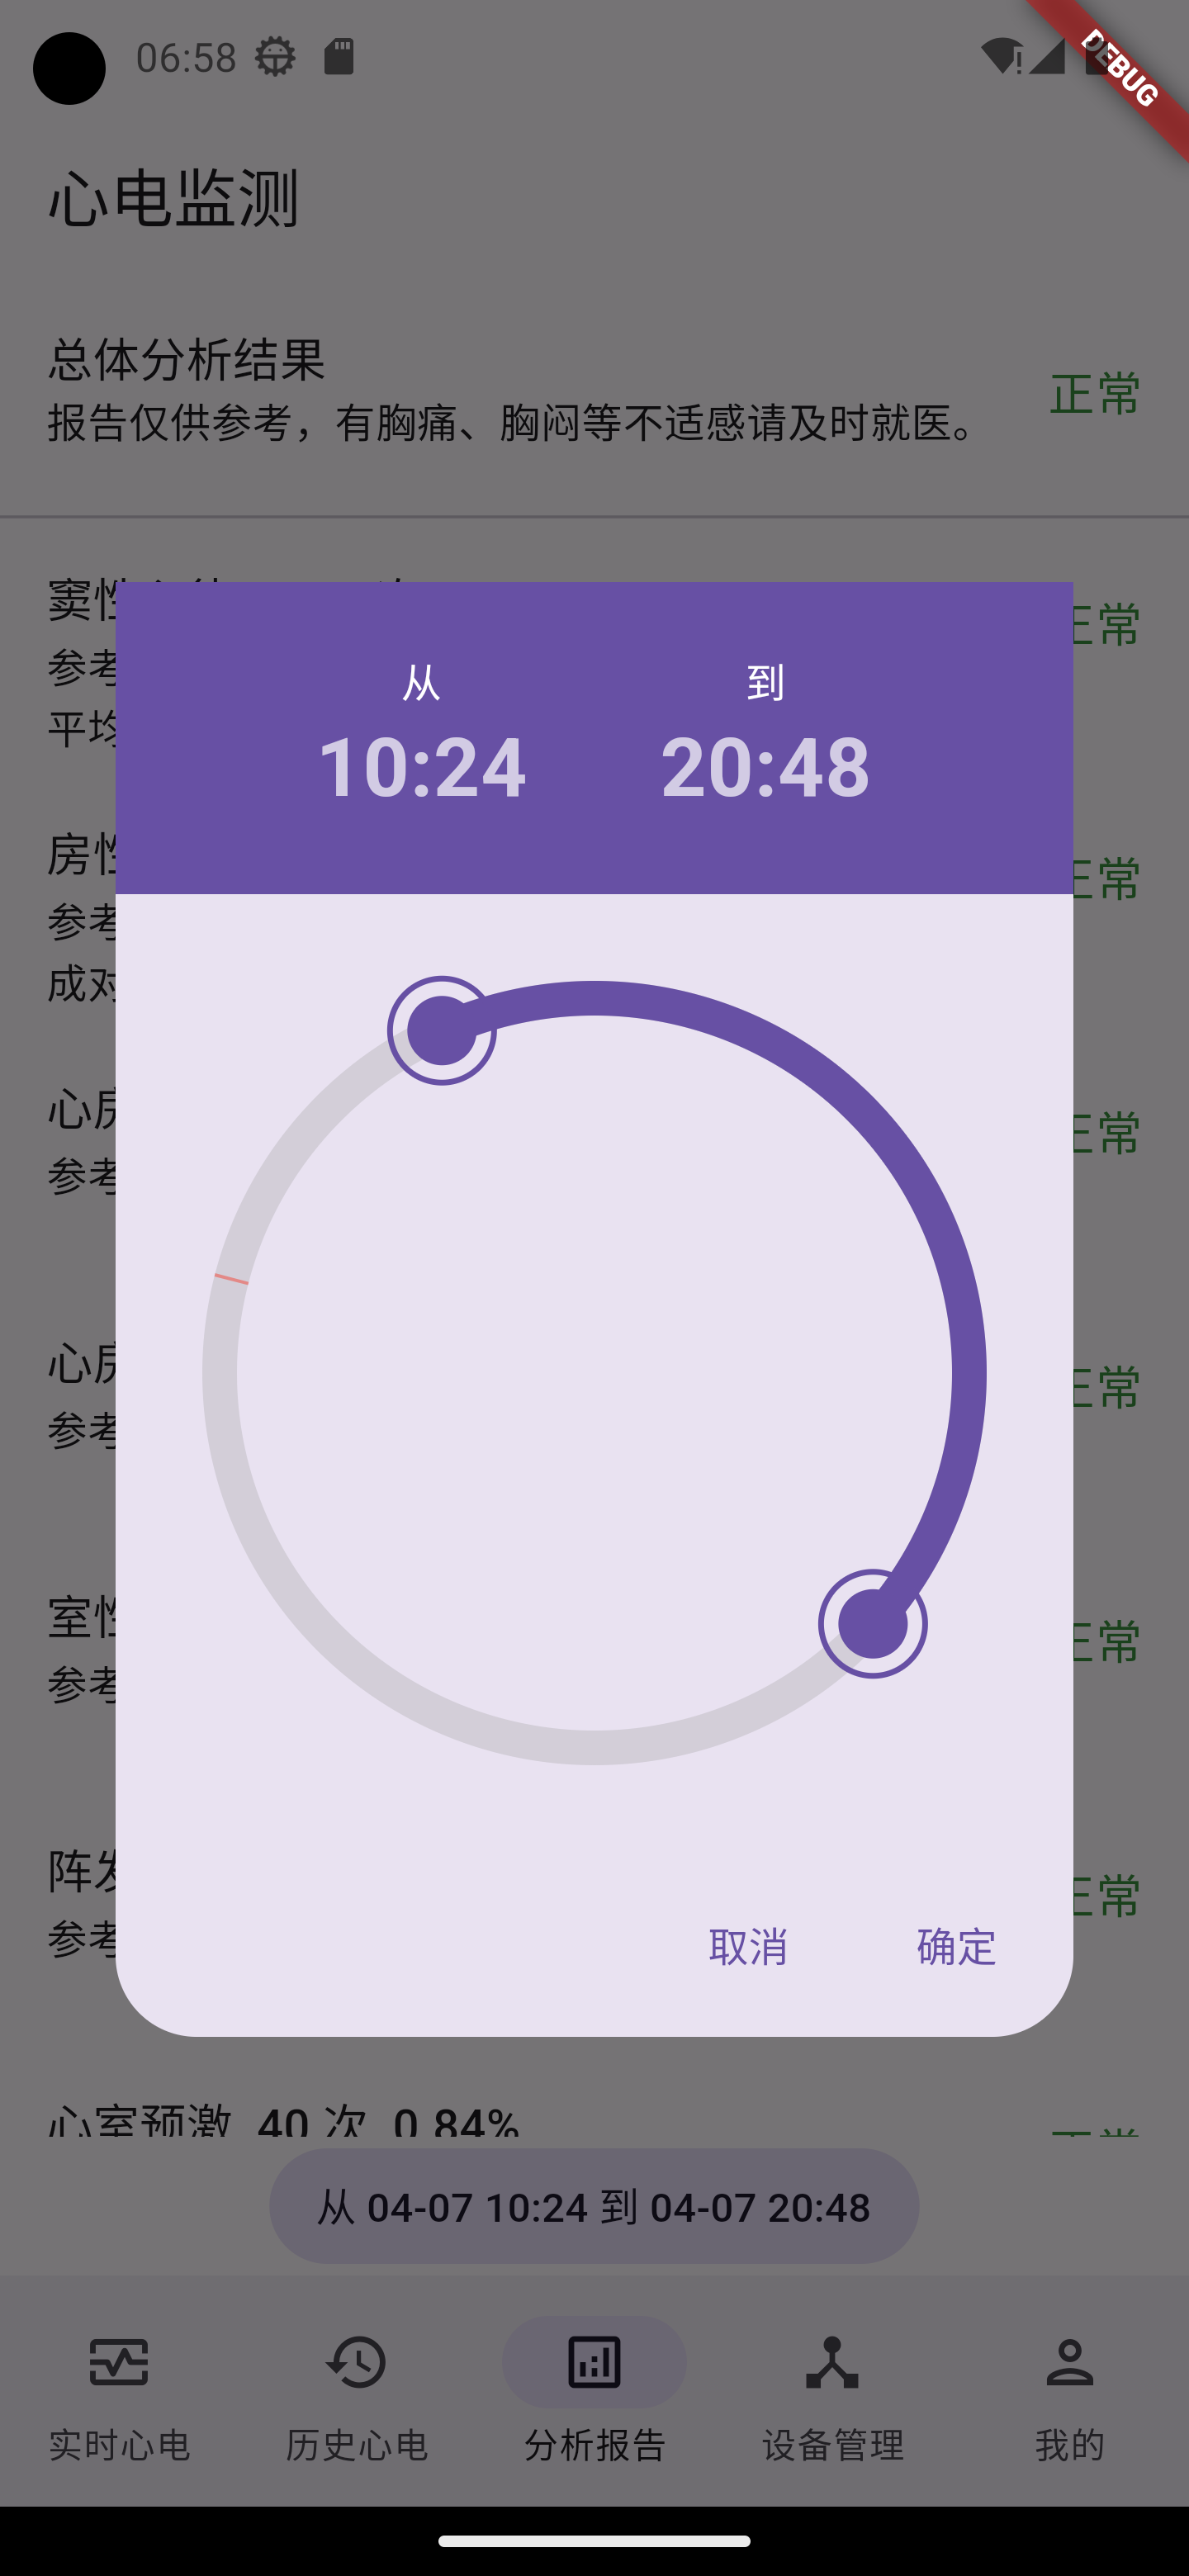
\includegraphics[width=.33\textwidth]{../assets/analytics-dialog}}
    \bicaption{分析报告界面的设计}{Design of the analytics page}
    \label{fig:analytics}
\end{figure}

该界面可以划分为分析报告展示与时间范围选择器两部分,另外点击心律类型可以展开心律类型详情界面。

\subsubsection{分析报告展示部分的设计}\label{subsubsec:analytics-display-design}

该部分区域整体上是一个可以上下滑动的列表。由于分析报告内容过多,在一个屏幕内完全展示会过于拥挤,所以使用了可滑动列表的形式。

最上方的一小条区域是线状进度指示器。由于难以确定生成分析报告所需的具体时长,所以该进度指示器是不确定进度的样式。另外,由于该部分有很多界面元素可以在获取到实际数据之前就确认其内容与位置,所以没有像历史心电界面那样使用屏幕中央的圆形加载进度指示器,而只是在最上方使用了线状进度指示器,并在加载时提前显示部分可以确定的元素,以减少加载前后的界面变化,提升用户对界面内容的确定感。在加载完成后,该区域并不会直接消失,而是会替换为不可见的与进度指示器高度相同的空白元素,以保证界面布局的稳定性,避免下方内容在加载完成后突然上移。

在进度指示器之下显示了所选时间范围的分析结果的总结,以右侧以带颜色的字体显示对分析结果的简要概括(“正常”、“心动过速”等),并在下方给出稍详细一些的解释。

总结区域的下方放置了一条分割线,用以分割总体分析结果与具体的心律类型分析结果,并在视觉上对总体结果加以适当强调。

在分割线之下,每个心律类型的分析结果都会显示在一个独立的区域中。首先以稍大的字体显示心律类型的名称、次数、占比,然后以小一些的字体给出该心律类型相关数据的正常范围作为参考值,第三行显示部分心律类型会具有的额外信息,如成对房早次数等;后两行的内容各自被限制在一行之内,溢出的内容会被以省略号替代,以提示用户可以点击该区域查看更多信息。此外,每个心律类型的右侧也和总结一样给出了对该心律类型分析结果的简要概括。

各个心律类型的区域都是可以点击展开查看详细信息的。通常而言,可点击区域应当使用按钮等样式加以指示,但当屏幕上的可点击区域过多时应该避免过多的装饰,以免造成视觉上的混乱。对于列表项的可点击性的指示,一种常见的做法是在右侧显示一个箭头,但在本界面中右侧已经被占据,不便添加更多元素。因此,本界面使用了其他方式来提醒用户心律类型可以点击。除上文所述的省略号外,该界面利用下方被截断的列表项指示该区域可以滑动查看更多内容,并在用户滑过心律区域时展示了水墨扩散的效果,如图~\ref{fig:ink} 所示,效果会从点击位置向四周扩散。水墨扩散效果在Material设计中用于各种可点击区域的反馈,可以提醒用户心律展示区域点击后能触发额外动作。

\begin{figure}[ht]
    \centering
    
\includegraphics[width=.5\textwidth]{../assets/ink}
    \bicaption{心律类型区域的水墨扩散效果}{Ink effect of the heart rhythm area}
    \label{fig:ink}
\end{figure}

\subsubsection{时间范围选择器部分的设计}\label{subsubsec:analytics-time-range-design}

时间范围选择器部分仅在中间包含一个填充色调按钮。因为需要明确提醒用户所示分析报告的时间范围,所以没有使用强调效果较弱的轮廓按钮和文本按钮。按钮中的文本指示了当前选择的时间范围。点击按钮后,会弹出时间范围选择对话框。

时间范围选择对话框的主体是一个圆环,用户可以拖动圆环上的两个点来选定分析范围的起止时间。为了不引起日期的混淆,当前时间(在圆环上显示为红色)不被允许包含在选择部分之中,这样可以保证用户所选的时间范围总是可以解释为过去24小时之内的某个时间段。

\subsubsection{心律类型详情界面的设计}\label{subsubsec:label-details}

心律类型详情界面的设计的如图~\ref{fig:label-details} 所示。除上方的心律名称和返回按钮外,界面由可滑动查看的列表构成。列表内容包括该心律类型的说明文本,以及心律出现的具体时间。为了保证每个时间都可以较容易点击到,时间之间留有适当的间隔。点击时间后,会跳转至历史心电的对应时间。

\begin{figure}[ht]
    \centering
    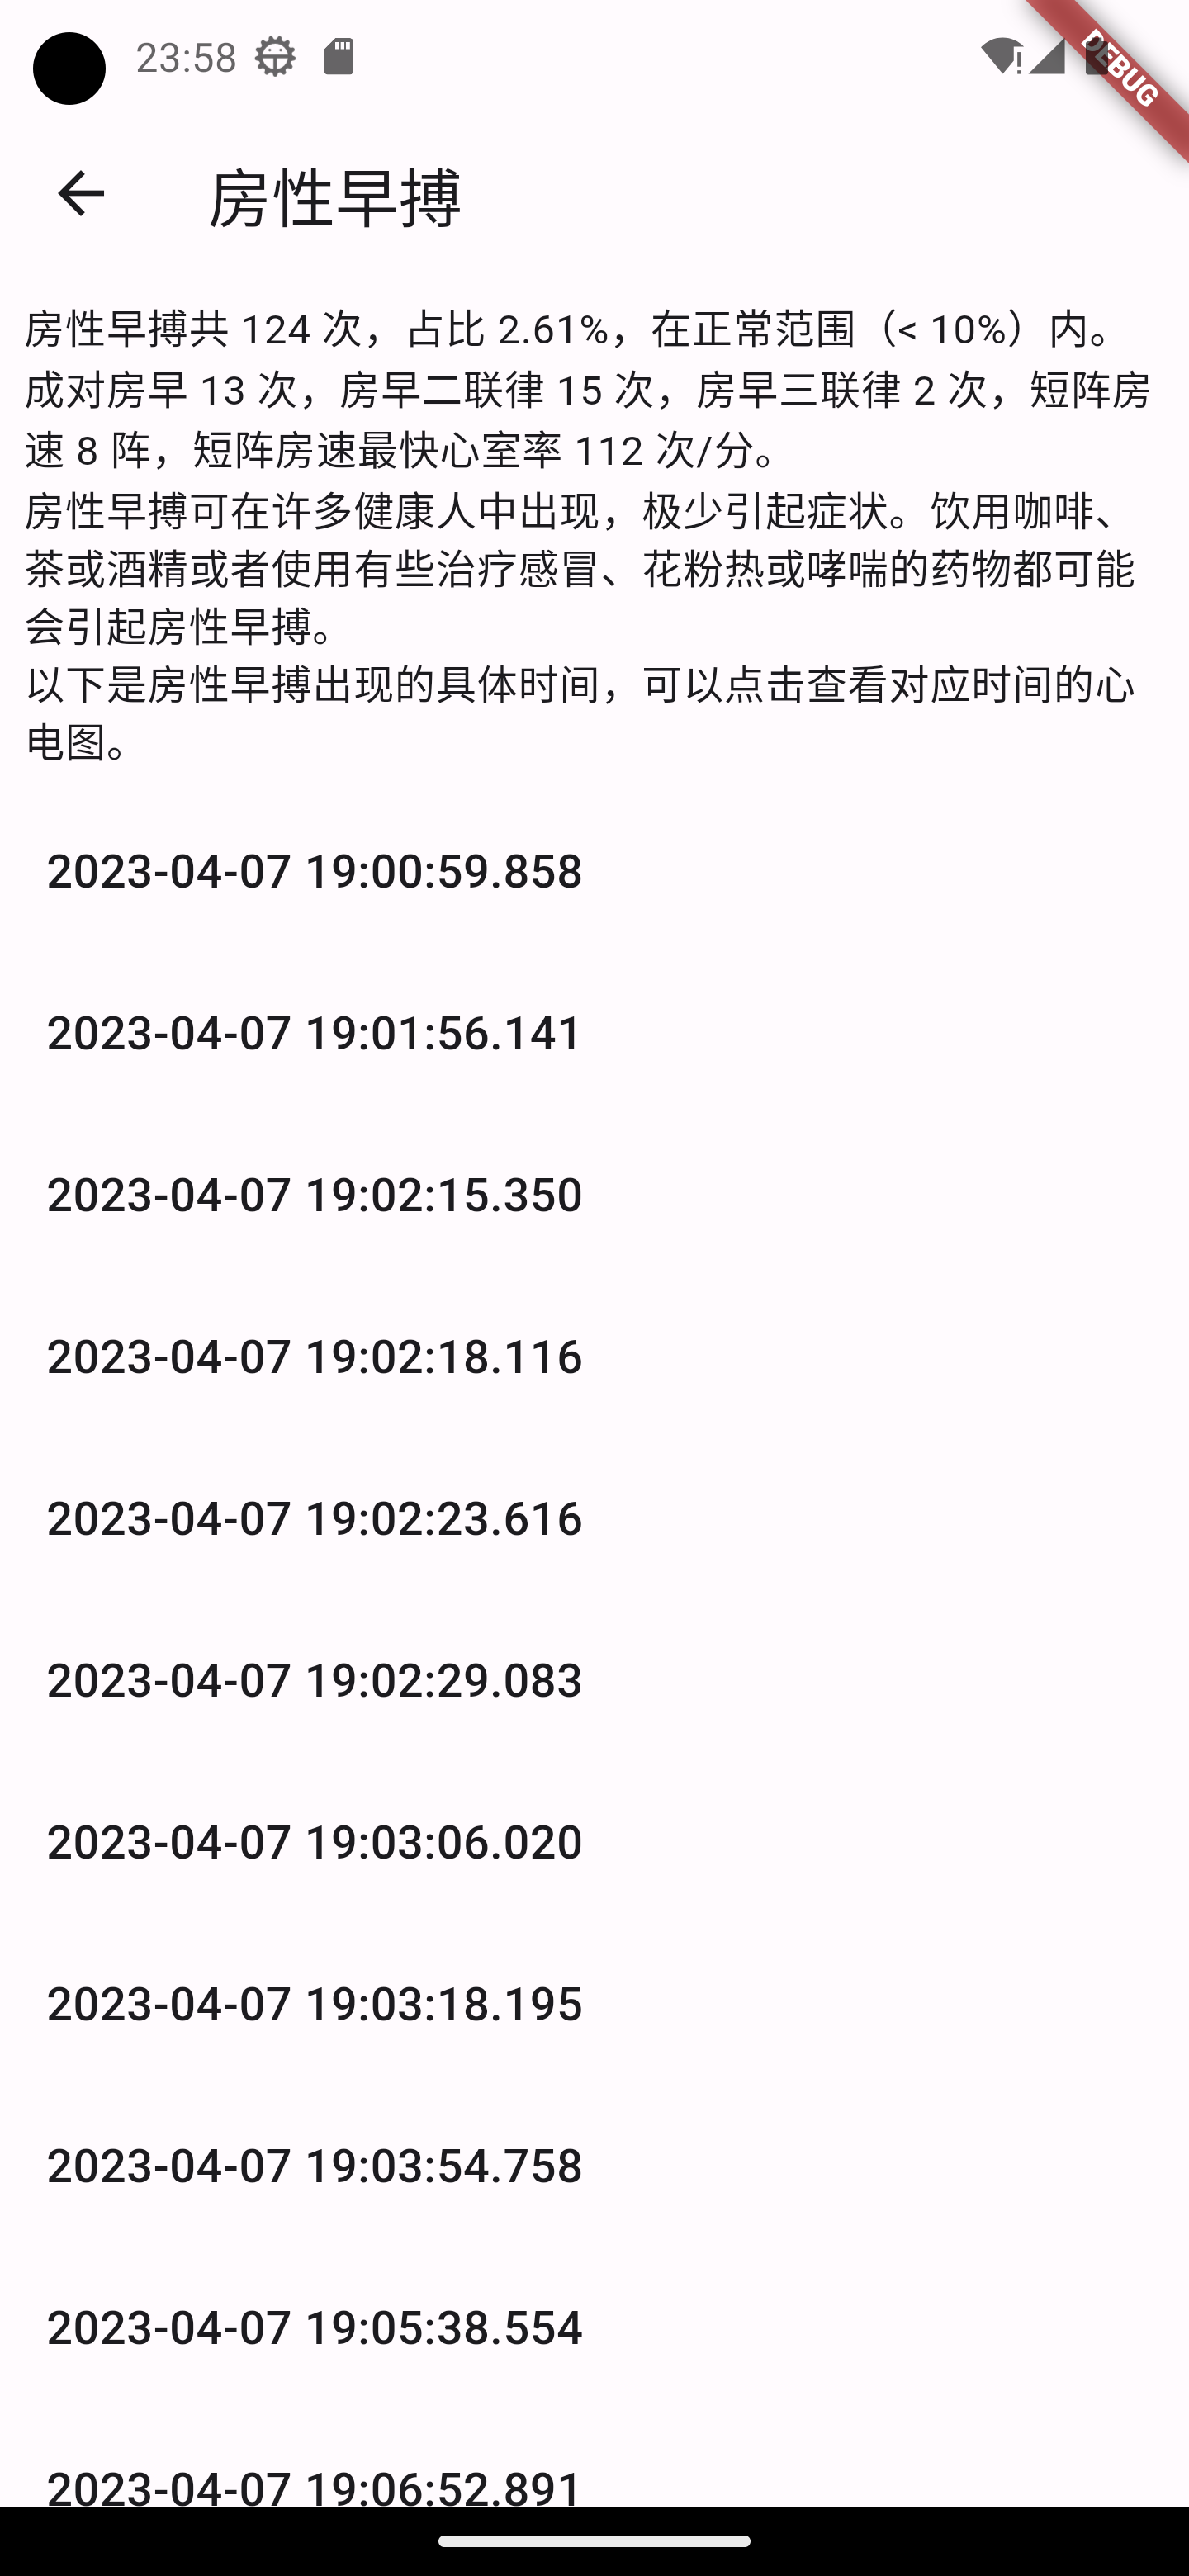
\includegraphics[width=.33\textwidth]{../assets/label-details}
    \bicaption{心律类型详情界面的设计}{Design of the heart rhythm details page}
    \label{fig:label-details}
\end{figure}

\subsection{设备管理界面的设计}\label{subsec:device-design}

\begin{figure}[ht]
    \subcaptionbox{已连接}{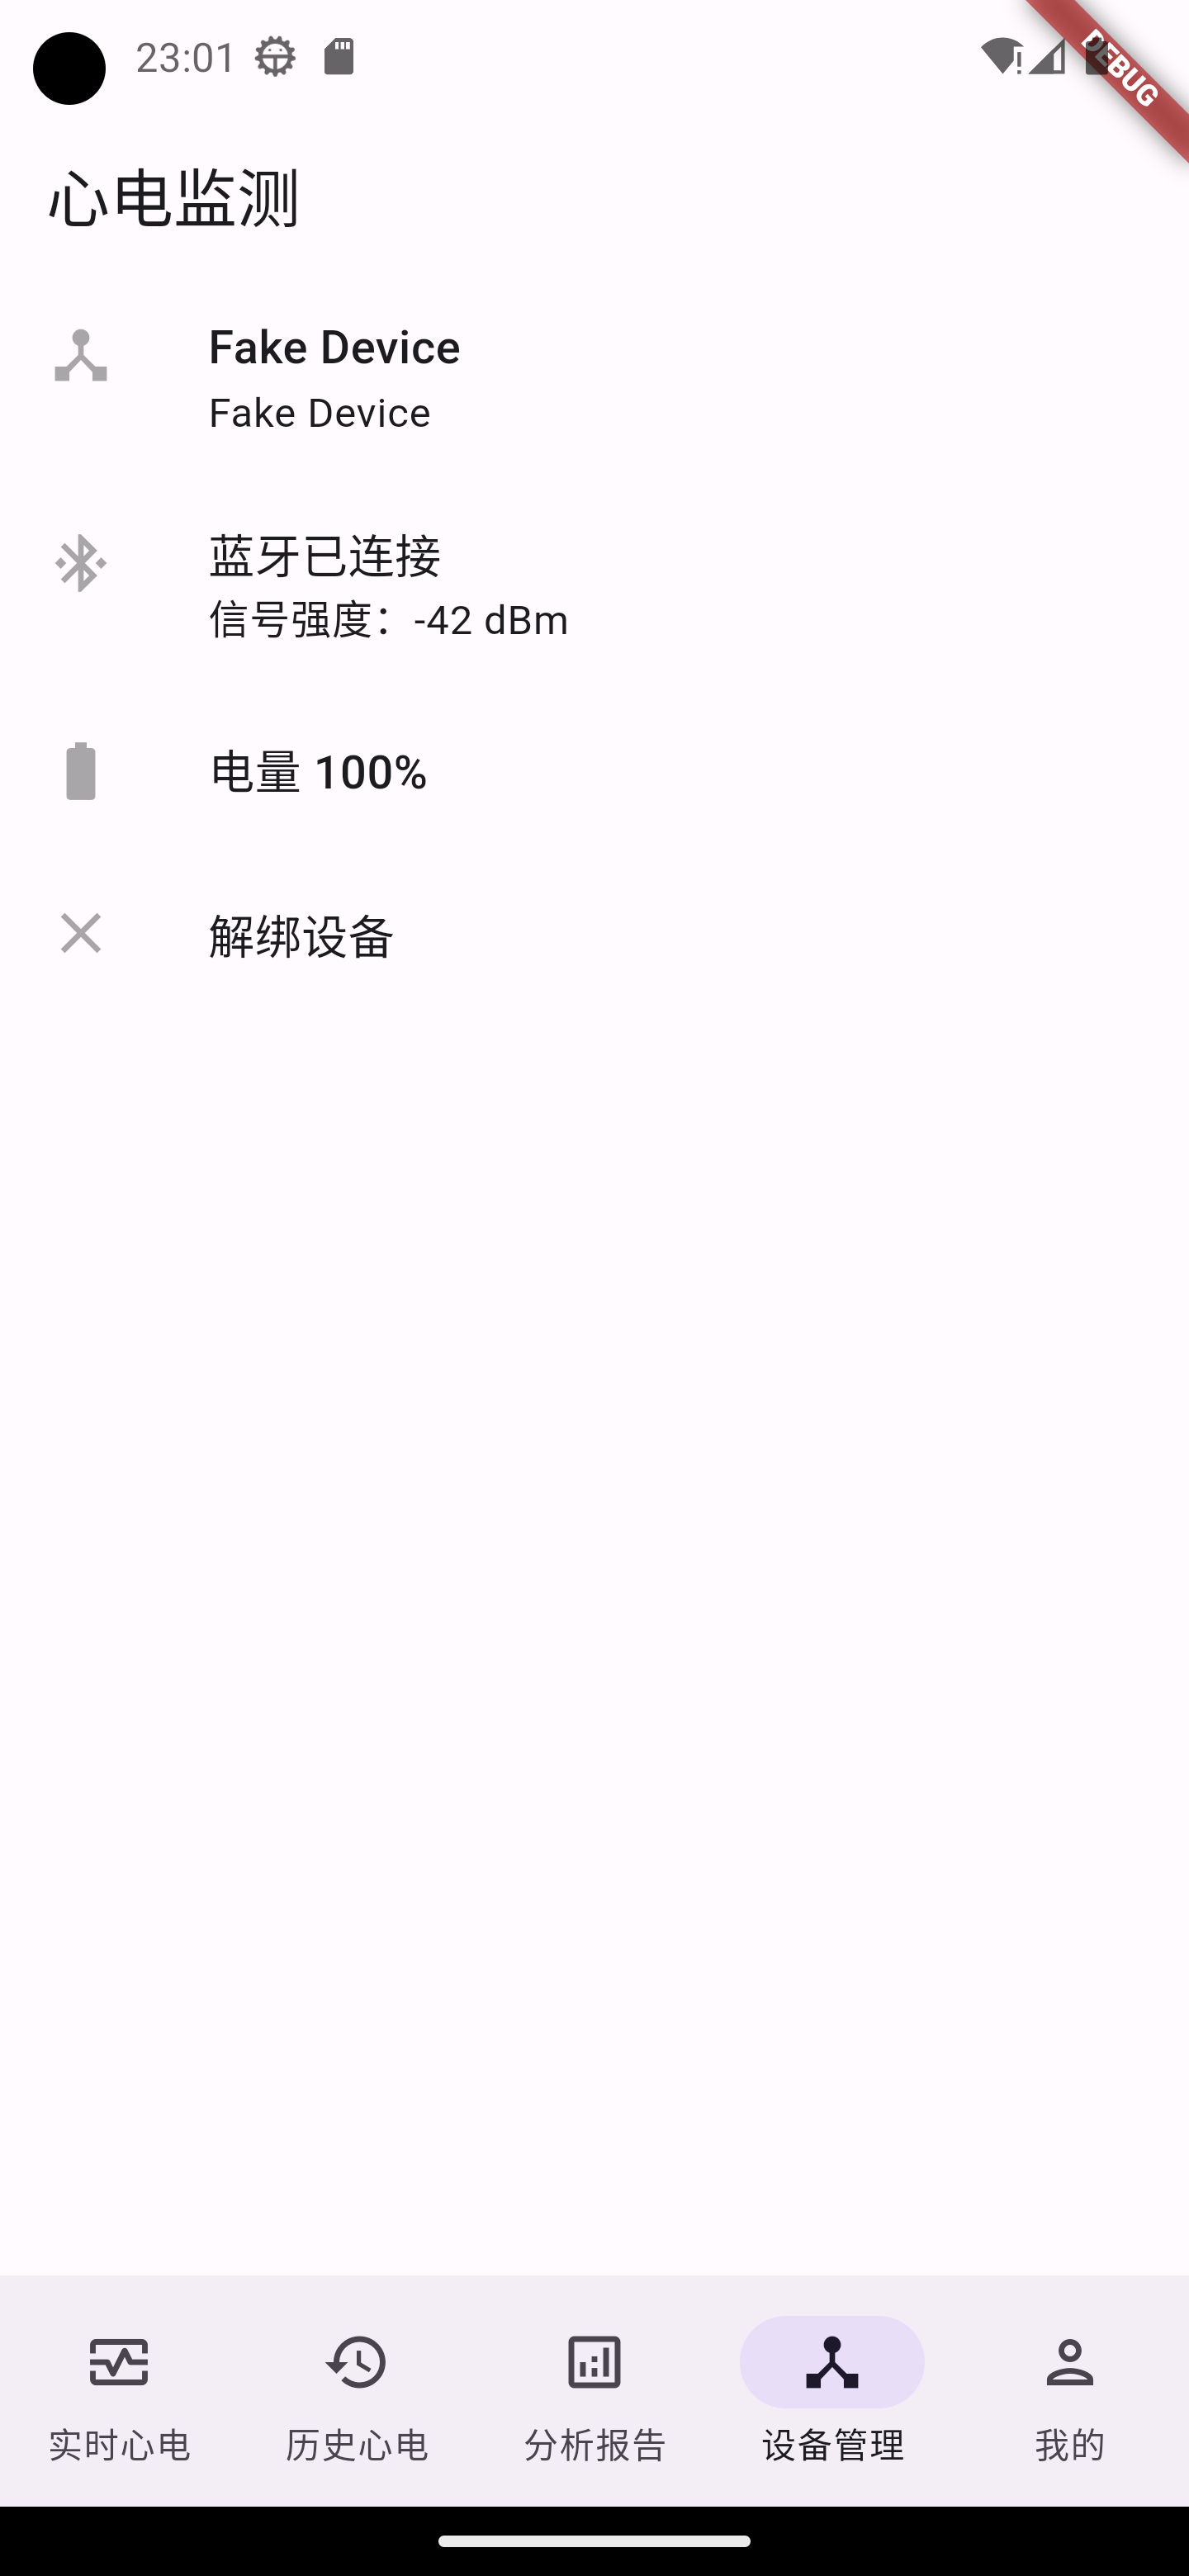
\includegraphics[width=.33\textwidth]{../assets/device-connected}}
    \subcaptionbox{连接新设备}{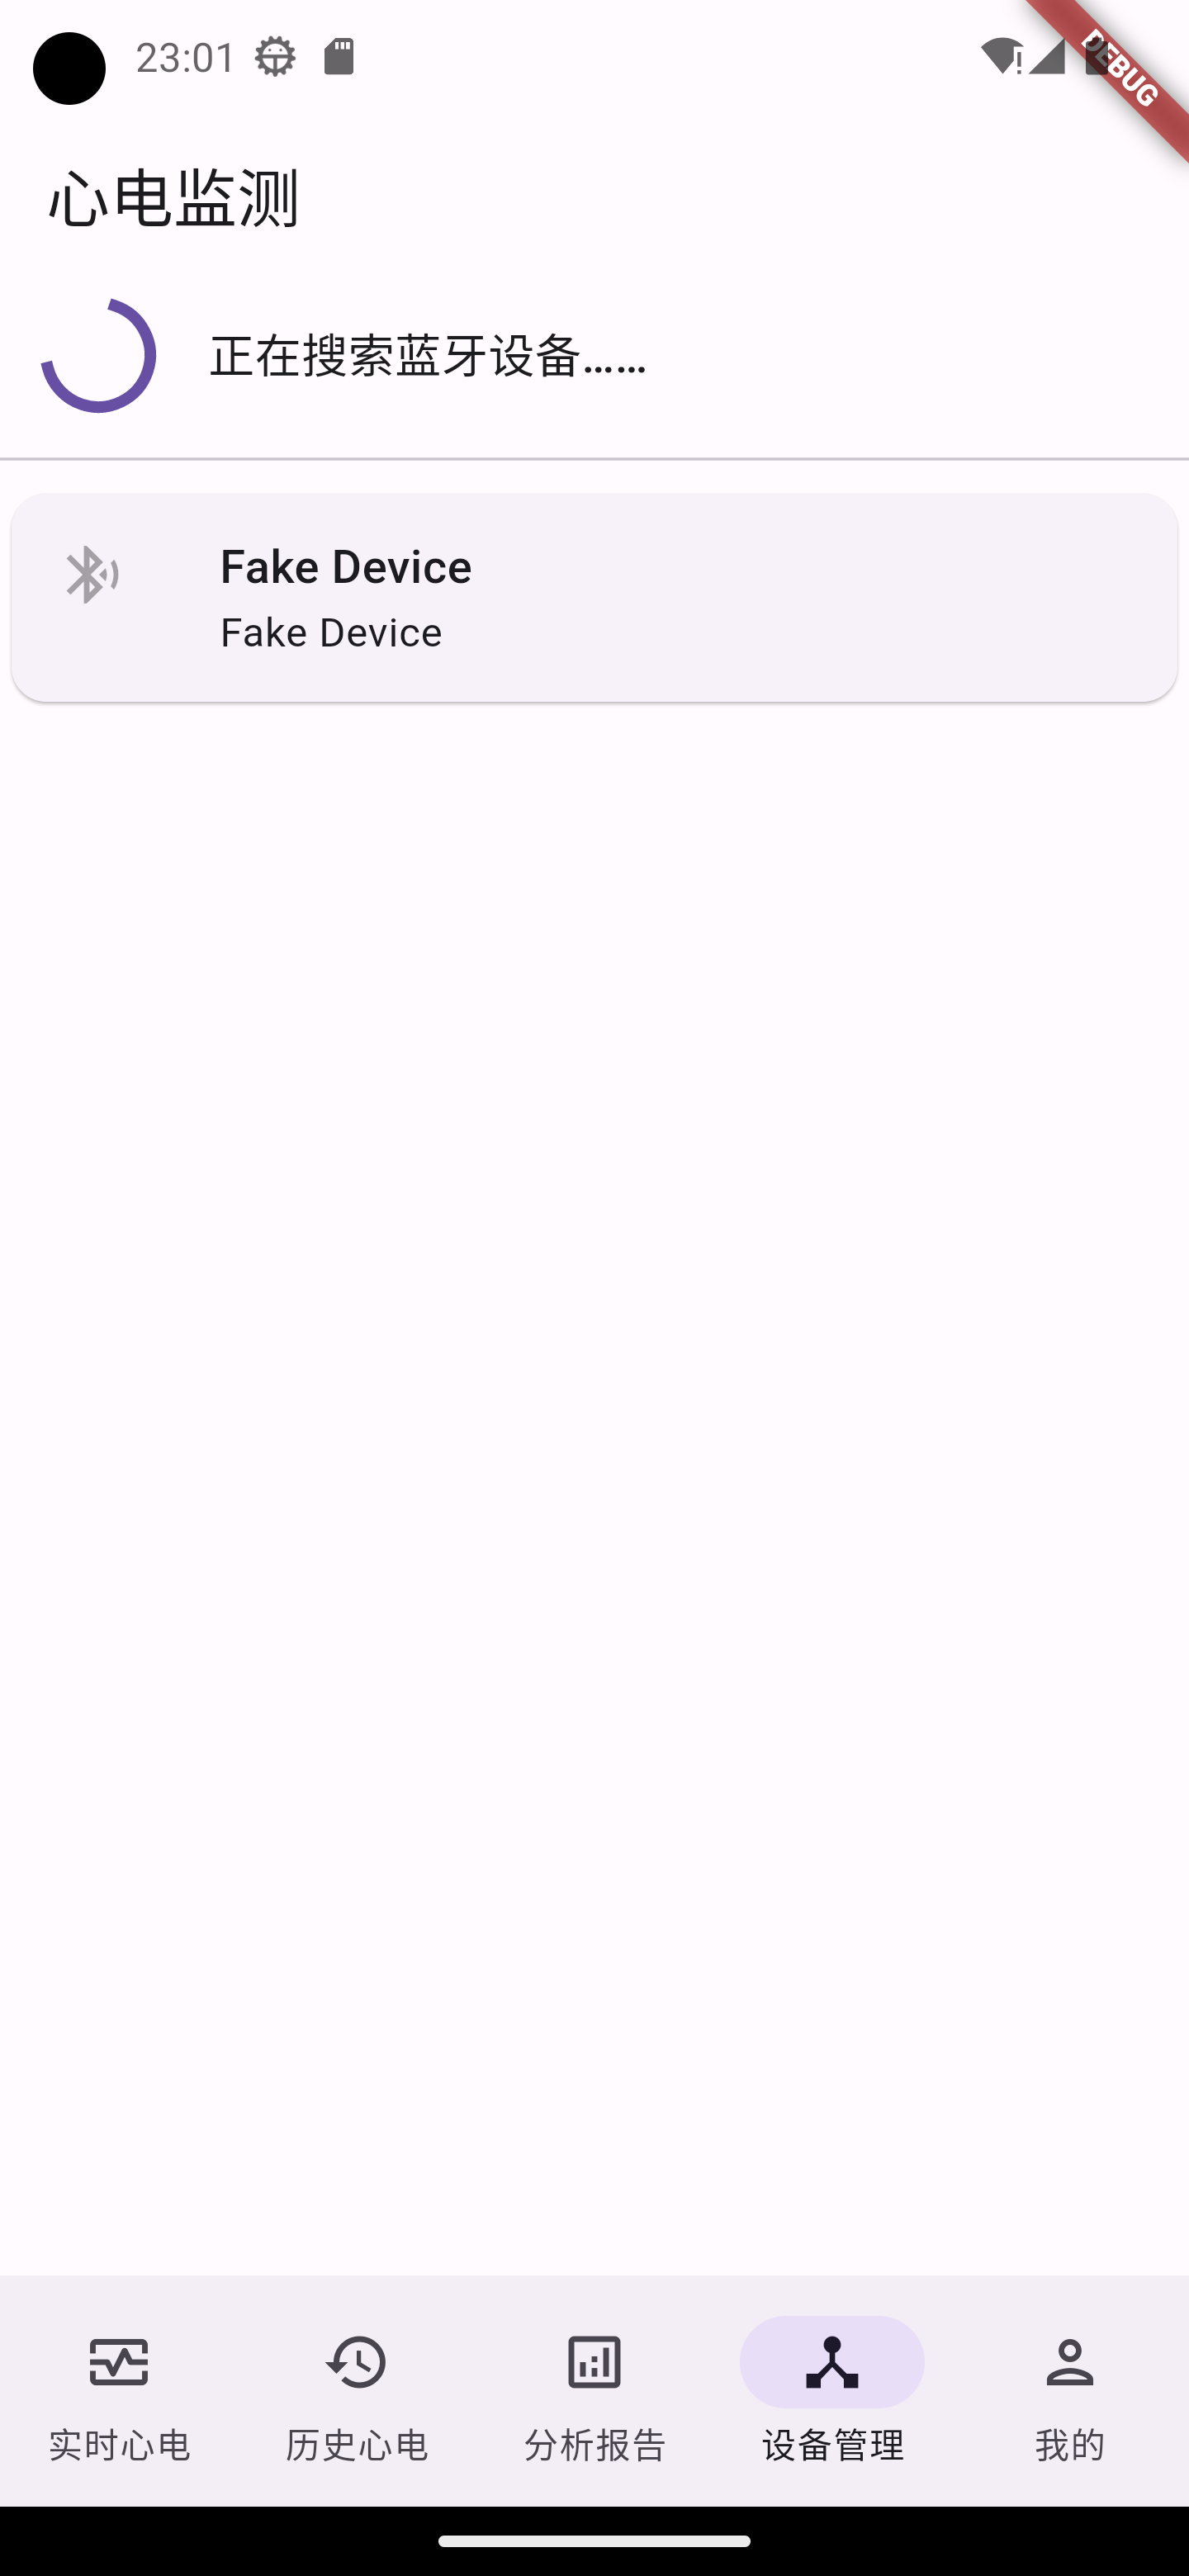
\includegraphics[width=.33\textwidth]{../assets/device-new}}
    \subcaptionbox{无可用设备}{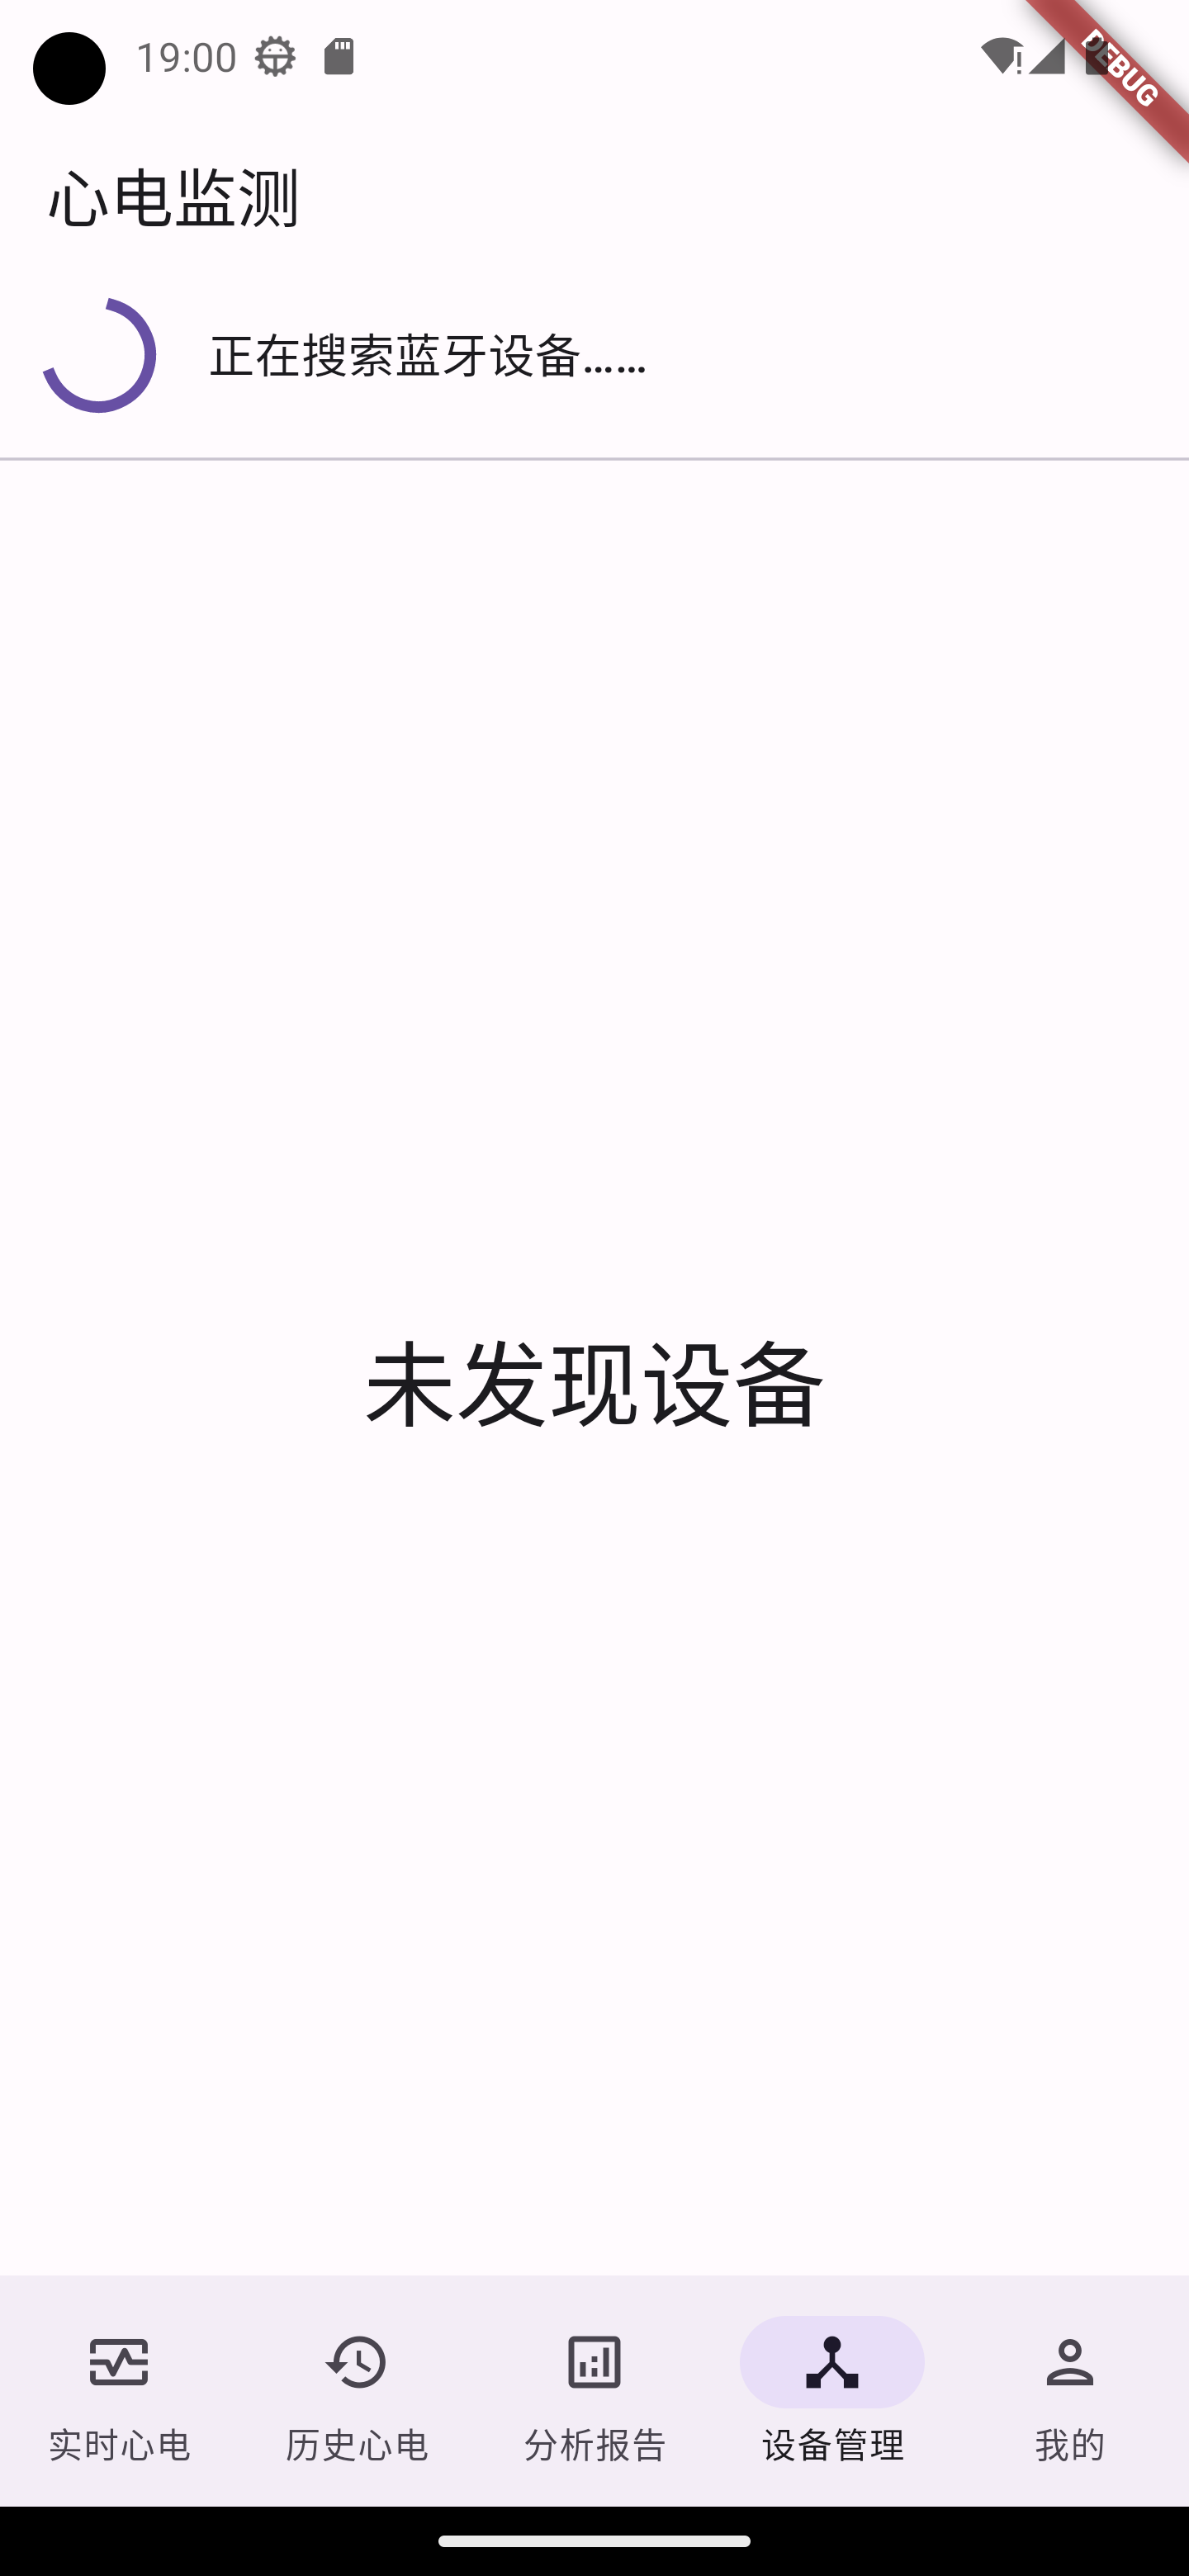
\includegraphics[width=.33\textwidth]{../assets/device-na}}
    \bicaption{设备管理界面的设计}{Design of the device page}
    \label{fig:device}
\end{figure}

设备管理界面的整体设计如图~\ref{fig:device} 所示。设备管理在导航栏中的图标是对心电监测设备所使用的电极片的简化表示。

该界面相比上述其他界面较为简单,分为已绑定设备和未绑定设备两种状态。

在已绑定设备的状态下,该界面会以列表形式展示设备的名称、型号、信号强度、剩余电量与充电状态等信息,并提供解绑设备的按钮。该按钮没有使用额外的设计来表示其可以点击,因为“解绑设备”这一文本本身已经足够明确地指示了该区域是可以点击的。

在未绑定设备的状态下,该界面会起到搜索并绑定设备的作用。界面上方展示“正在搜索蓝牙设备”的提示并显示了不确定进度的圆形进度指示器,之后有一条分割线,下方则展示了搜索到的设备列表。列表中的每一项都表示了一个搜索到的蓝牙设备(由于Android和iOS模拟器均不支持蓝牙功能,截图中仅显示了一个模拟设备),并以带阴影的卡片的样式来显示其可以直接点击,而没有额外放置绑定按钮,以使界面设计更加简洁。

\subsection{其他功能的设计}\label{subsec:other-design}

应用中有一些用户不常主动访问,但仍然应该提供的界面,一些相关界面的设计如图~\ref{fig:other} 所示。

\begin{figure}[ht]
    \subcaptionbox{我的}{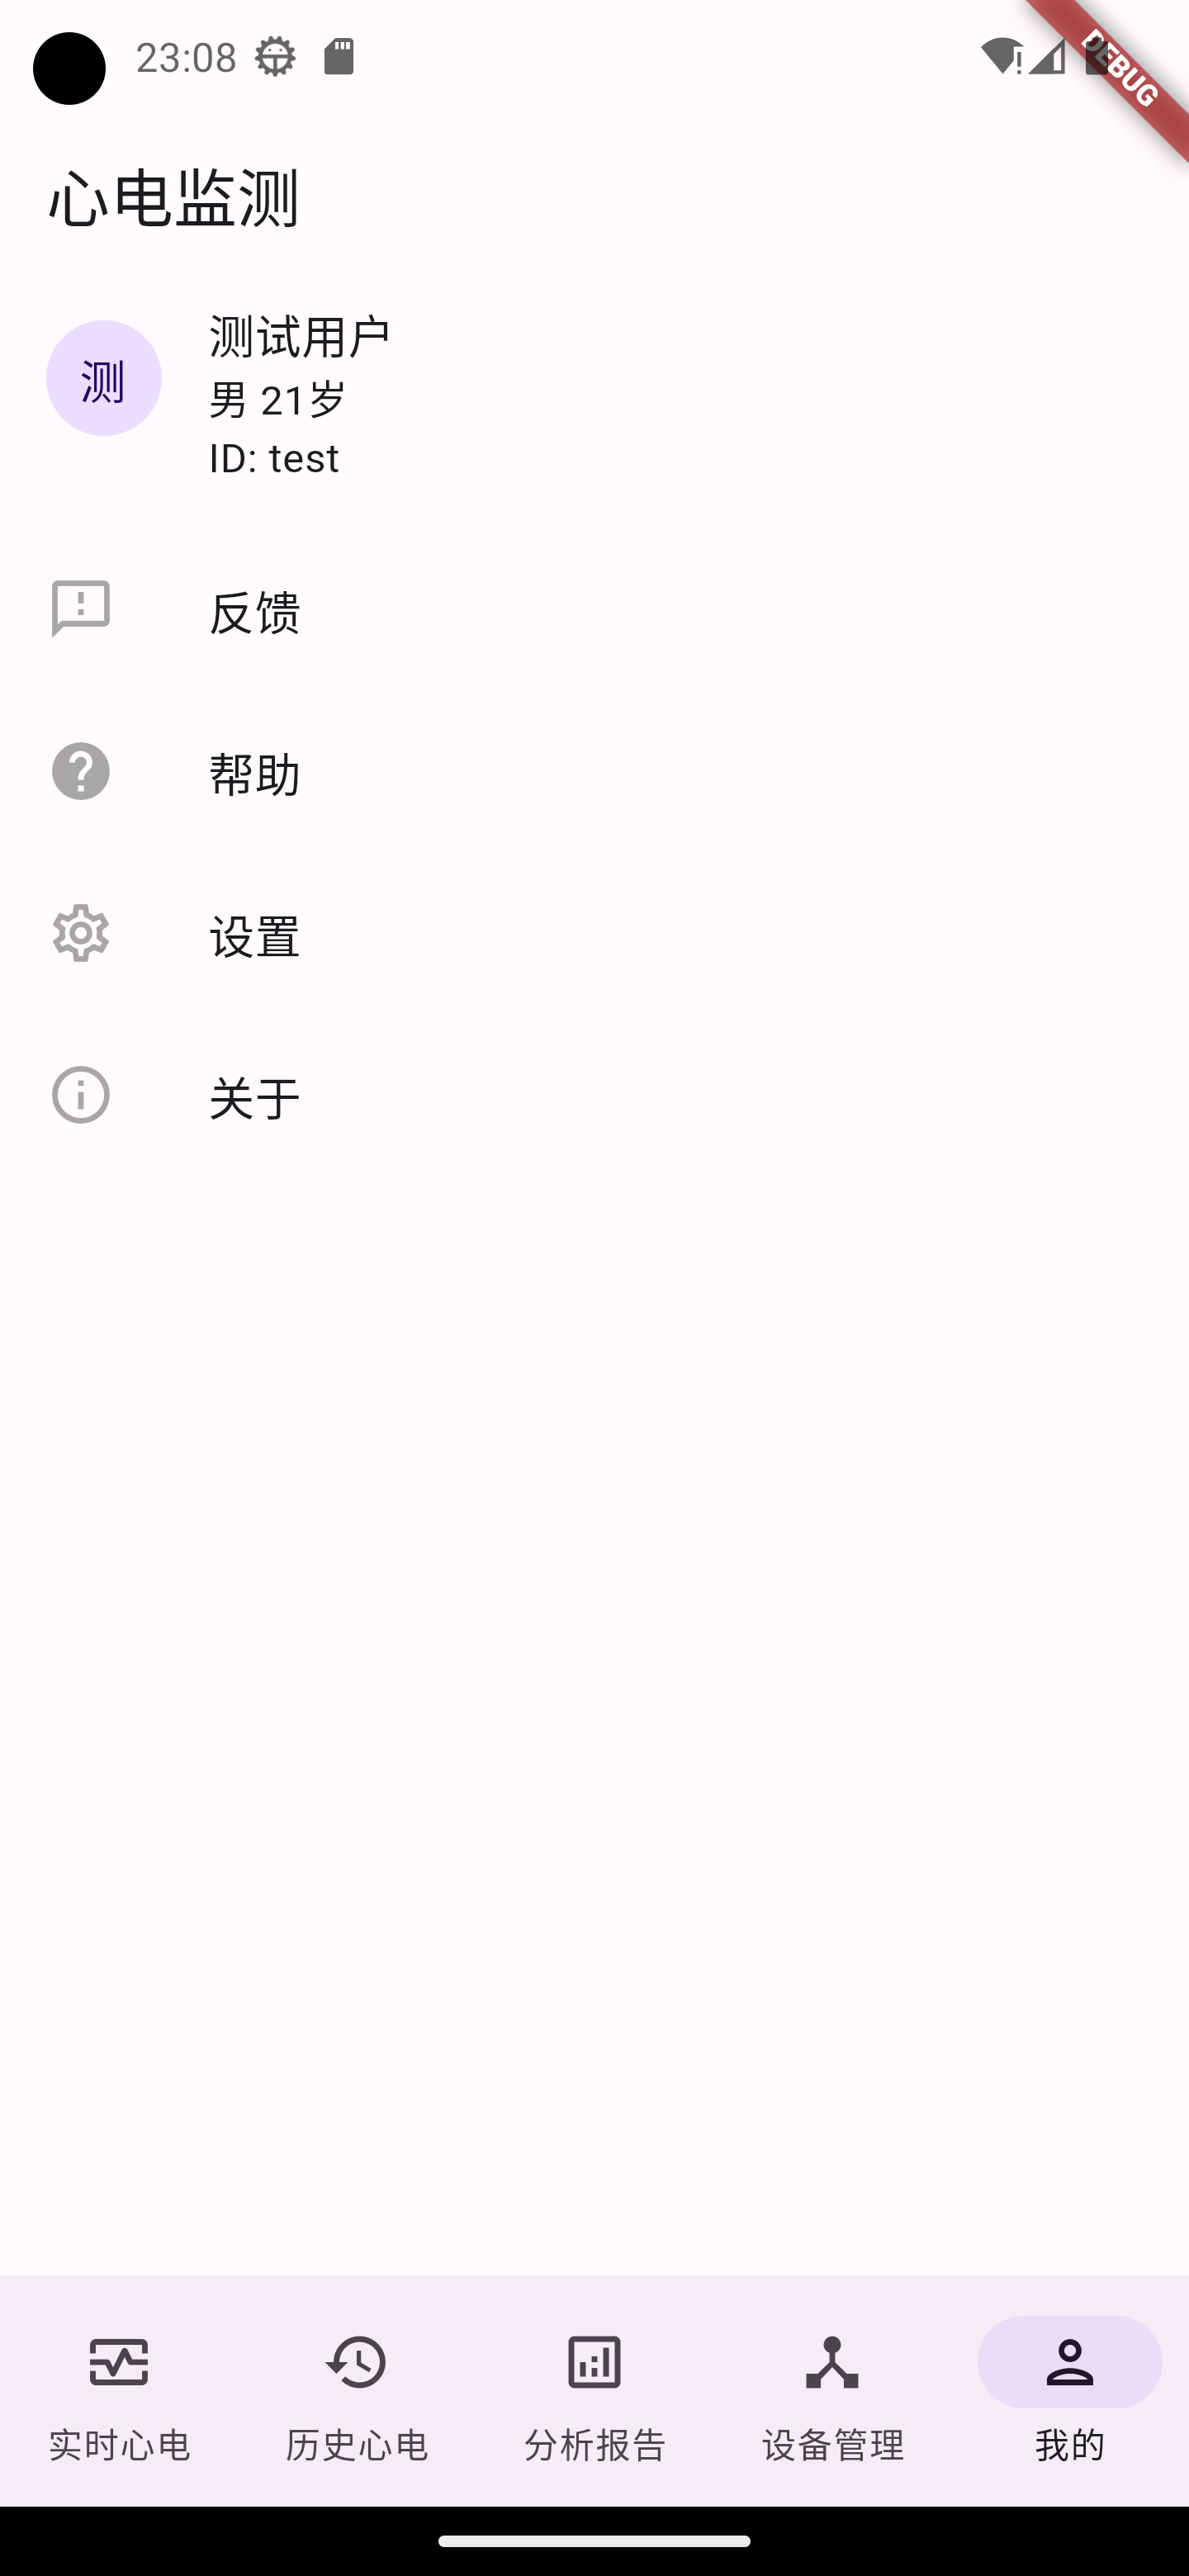
\includegraphics[width=.33\textwidth]{../assets/me}}
    \subcaptionbox{设置}{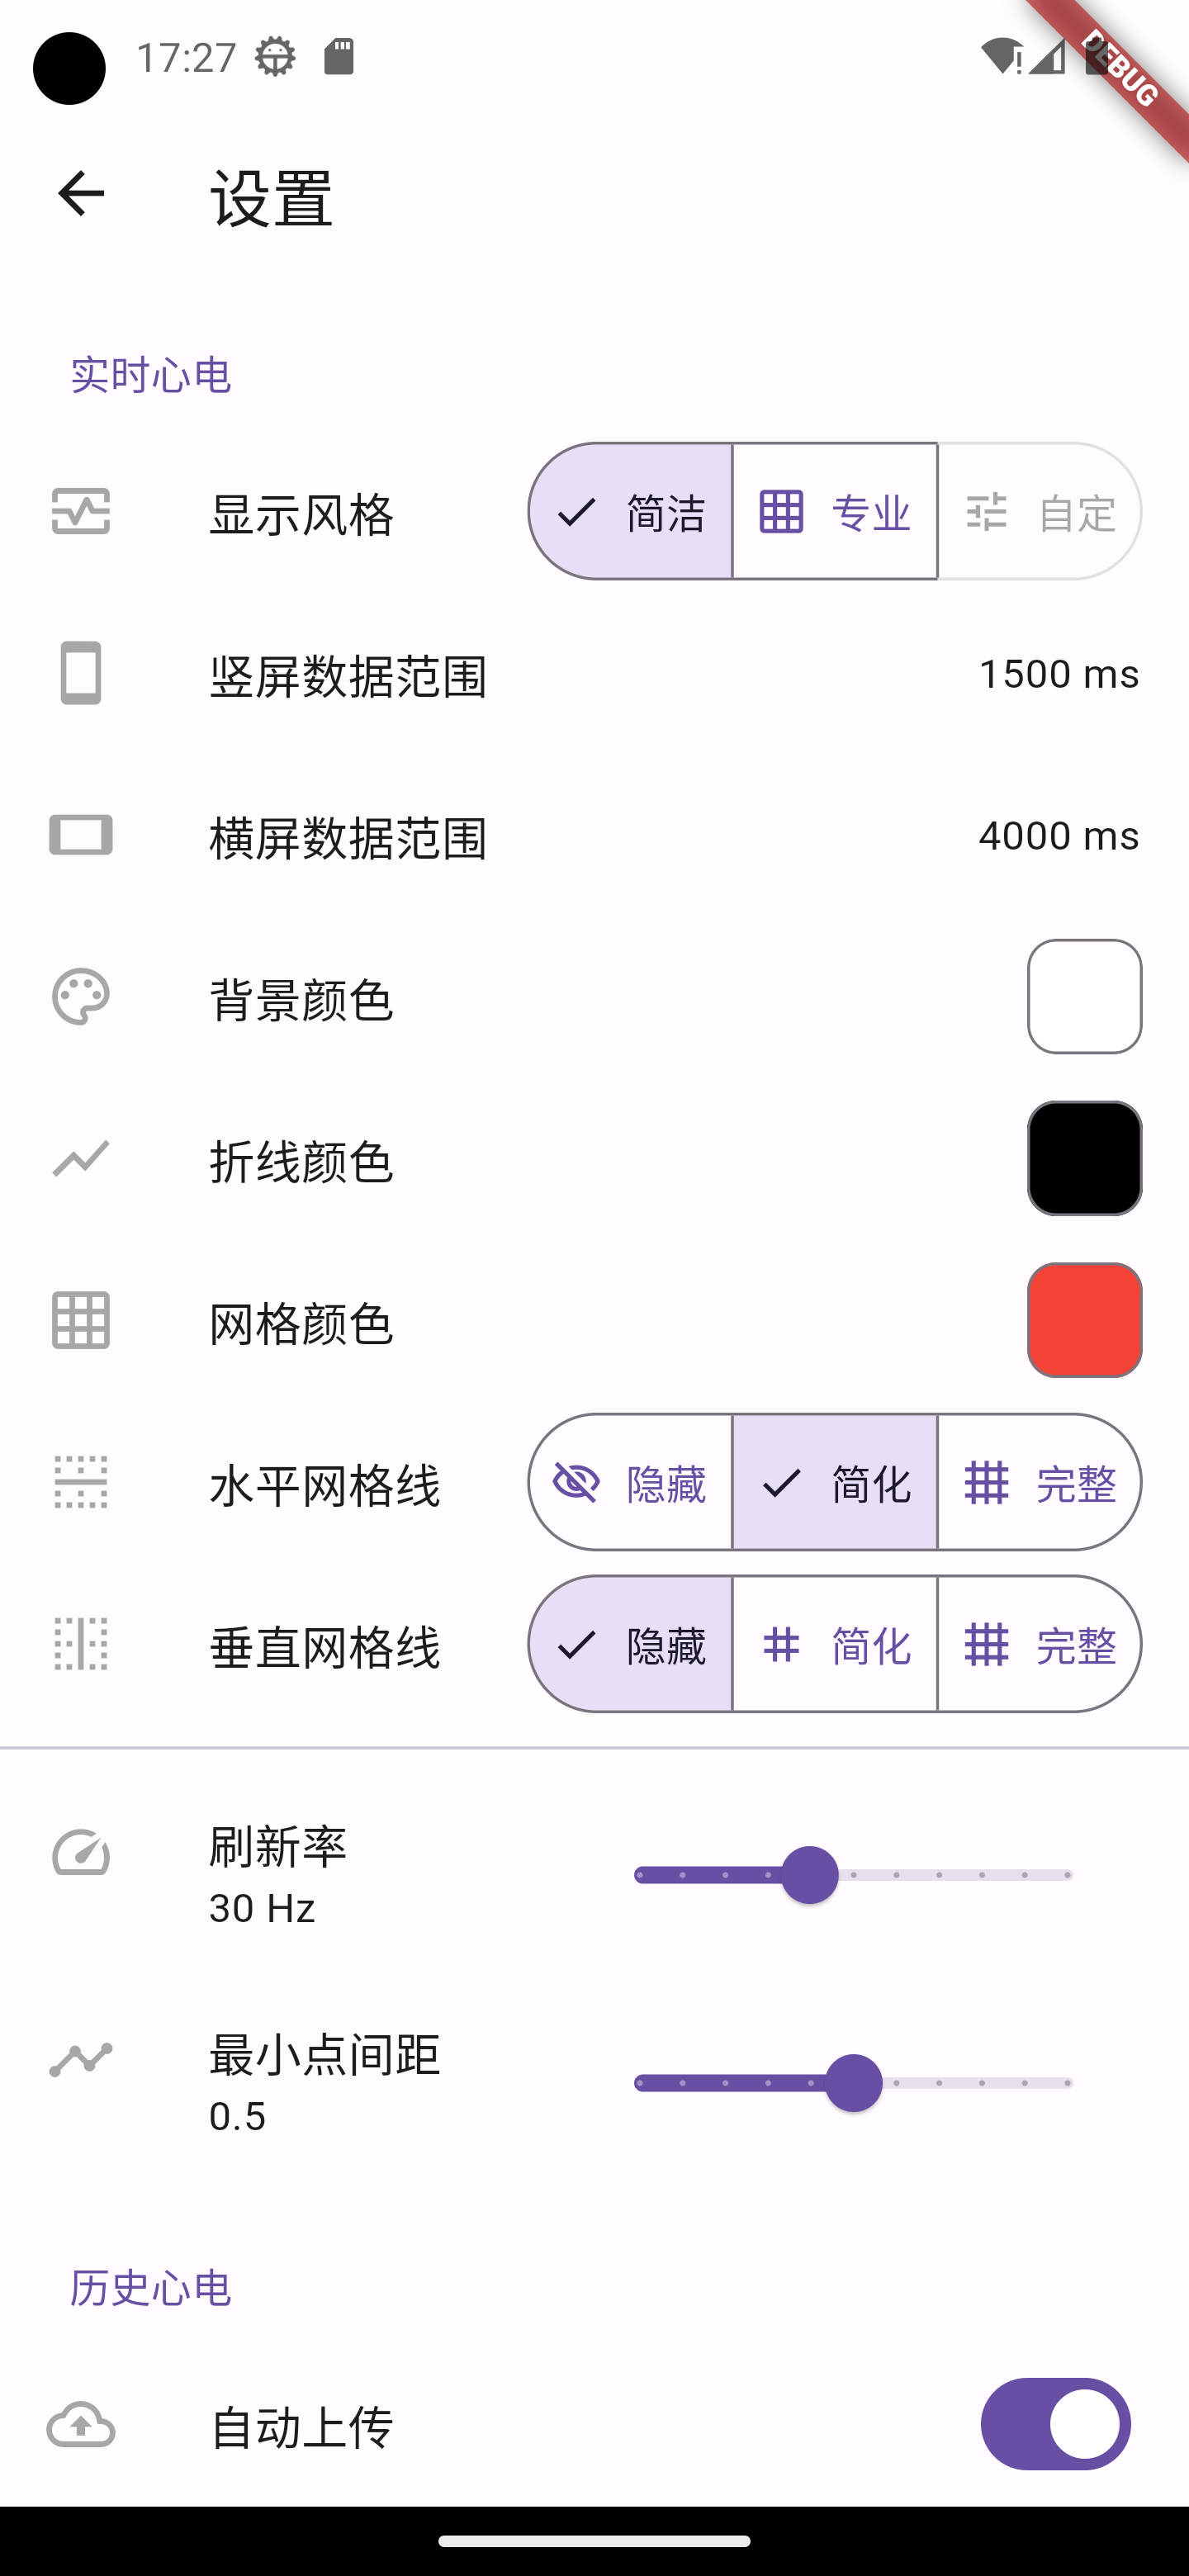
\includegraphics[width=.33\textwidth]{../assets/settings}}
    \subcaptionbox{许可}{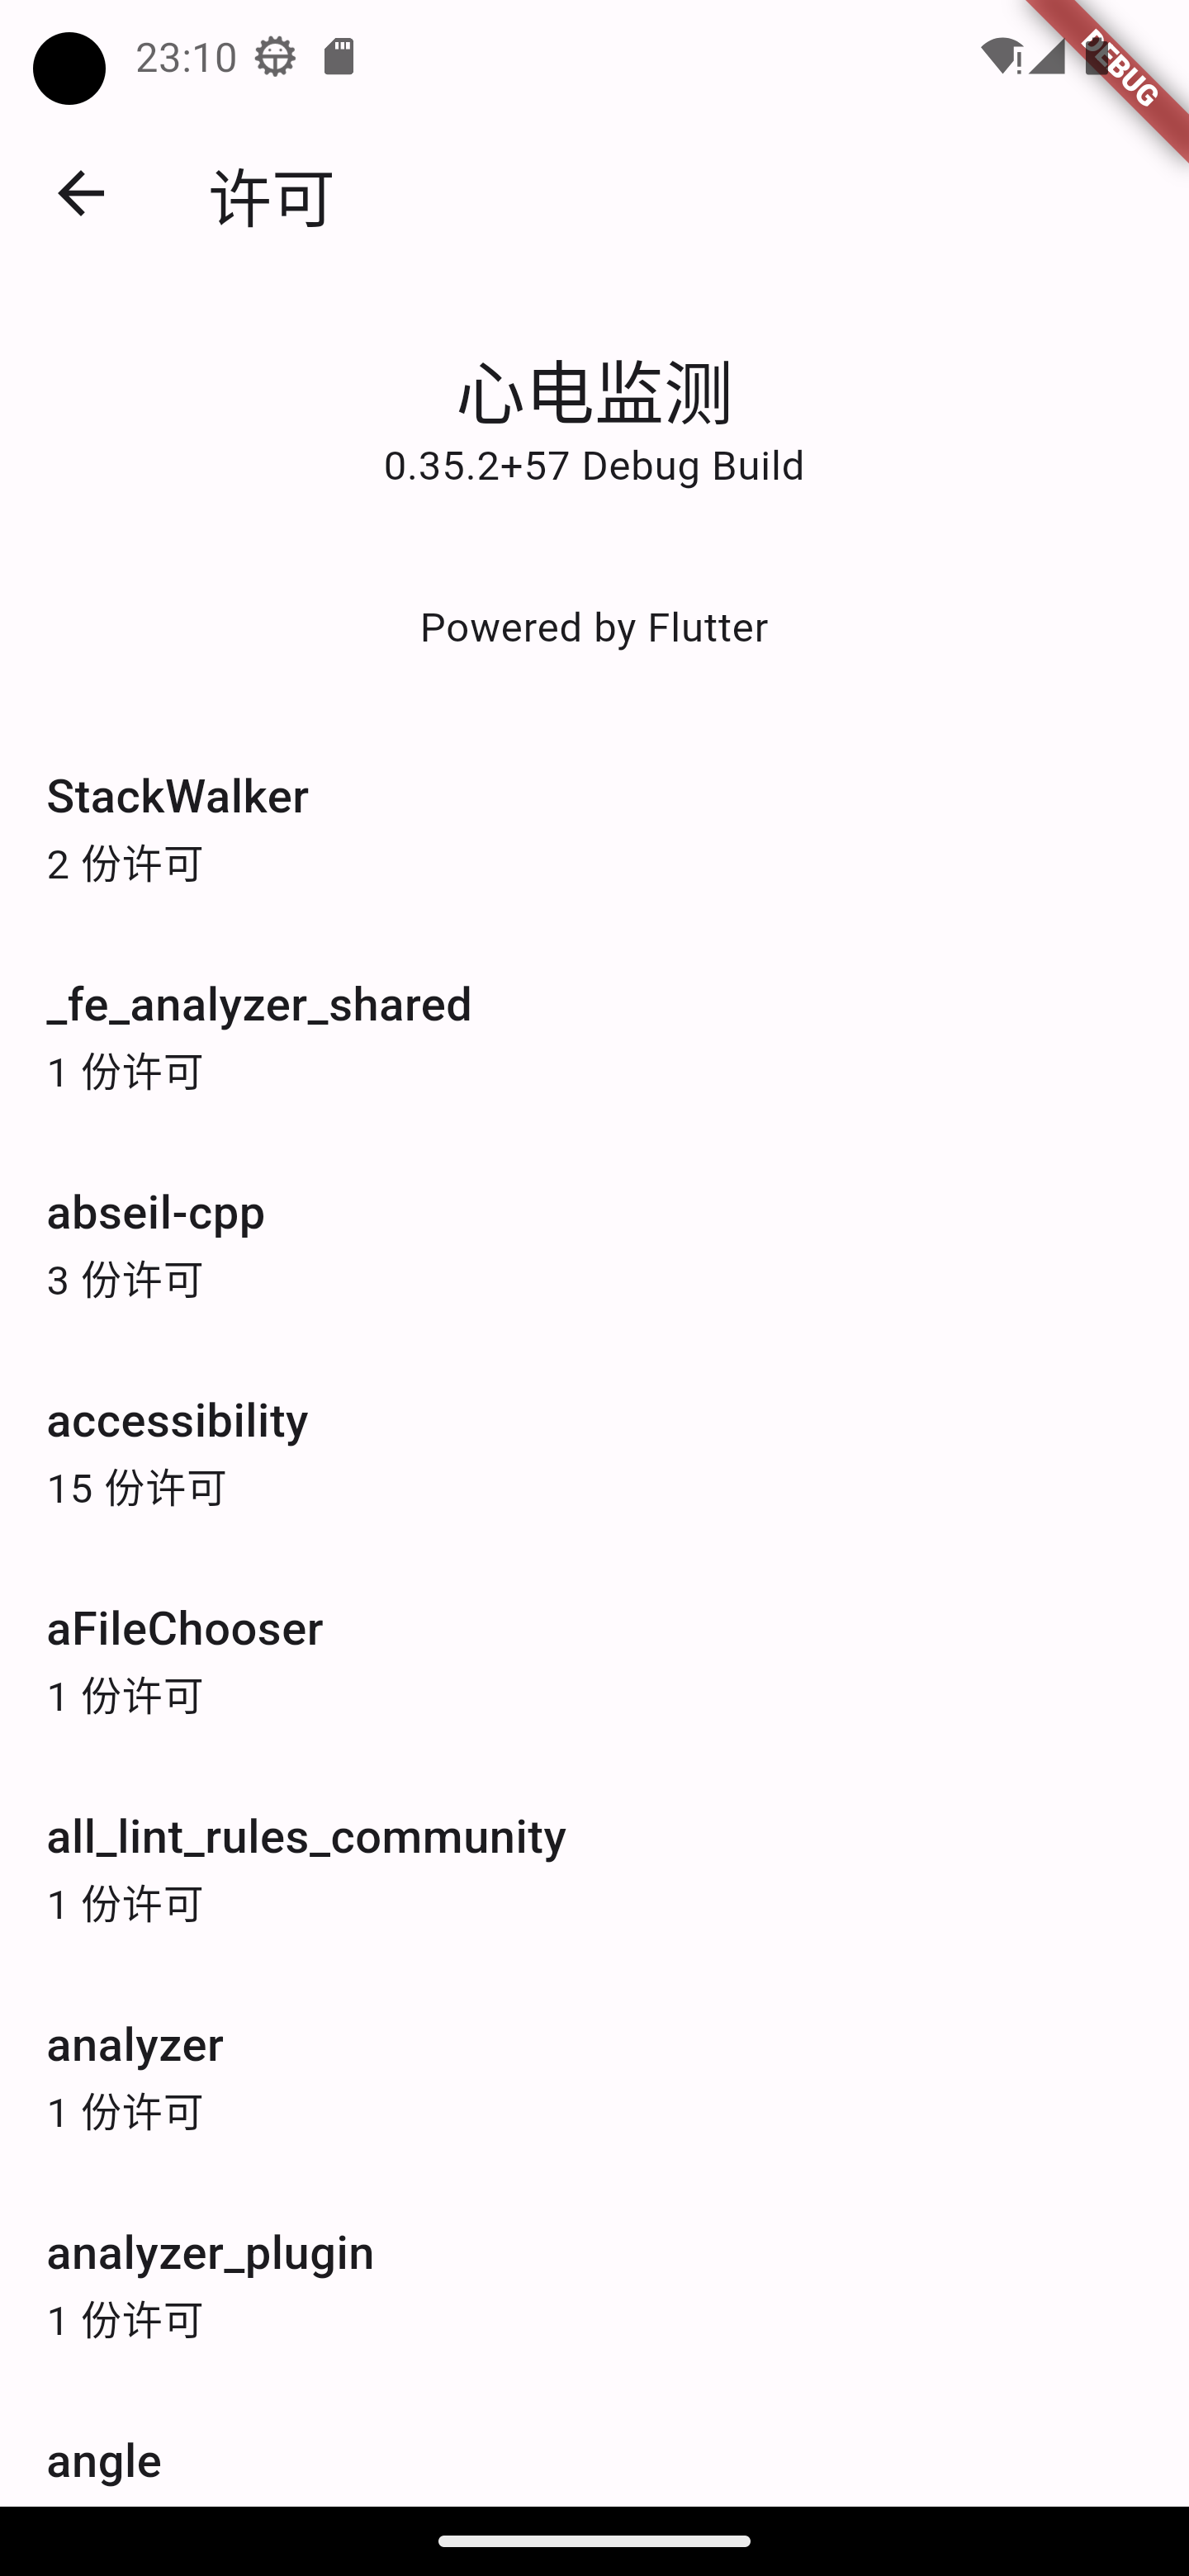
\includegraphics[width=.33\textwidth]{../assets/license}}
    \bicaption{其他界面的设计}{Design of the other pages}
    \label{fig:other}
\end{figure}

\subsubsection{我的界面的设计}\label{subsubsec:me-design}

我的界面提供了其他所有界面的入口,在导航栏中的图标是用户头像的抽象表示。该界面以列表形式展示其内容。用户项目显示了当前用户的头像、姓名、性别、年龄、ID等信息,由于可以复用Web端(同课题下的另一个子项目)的用户管理相关的内容,所以并未对用户界面进行专门设计。反馈、帮助按钮会在点击后打开对应的网页。设置按钮会在点击后打开设置界面。关于按钮会在点击后显示包含应用自身的版本、构建模式等信息的对话框,并提供更新日志与许可信息的入口。

\subsubsection{应用设置界面的设计}\label{subsubsec:settings-design}

应用设置界面为常见的列表形式,划分为多个部分,每部分有一个小标题。设置项目均使用了图标、标题、输入组件的形式来展示,有部分如滑动条等的设置项目因不方便在输入组件直接展示当前状态而添加了副标题。而颜色选择器等所需面积较大的输入组件则有缩小形式与完整形式,缩小形式仅指示当前状态,点击后会在弹出的对话框中显示完整形式。

\subsubsection{许可界面的设计}\label{subsubsec:license-design}

通常而言,用户并不会有查看应用程序所使用的各个开源包的许可协议的需求。但是,由于多数许可协议要求在应用程序中提供许可协议的副本,因此应用程序中必须提供该界面的入口。该界面以列表形式展示其内容。许可界面的每一项都是一个开源包,点击后会在弹出的界面中显示该开源包的名称、作者、许可协议等信息。此外,该界面的上方也显示了本应用的名称、版本和构建模式的信息,并显示了“Powered by Flutter”的标识。

\subsubsection{界面过渡动画的设计}\label{subsubsec:transition-design}

界面过渡动画是连接单个元素或应用程序全屏视图的短动画,是出色的用户体验的基础,可以帮助用户感知到应用程序的界面设计逻辑。由于在无法插入动态图片或视频的情况下较难充分展示界面过渡动画的实际效果,因此本文只作简短说明。

应用在心律类型详情界面的开启与关闭过程中使用了容器转换。当用户点击心律类型区域后,该区域会逐渐扩展至全屏,并将内容渐变为心律类型详情内容,关闭时则反之。这使得各个界面之间的关系清晰明确,加强了分析报告界面与心律类型详情界面的关联感。

在历史心电的所选时间改变后,使用了水平滑动效果,以提醒用户心电图是发生了水平移动。由于各个心拍之间的图像可能较为相似,如果没有该动画,用户可能会产生心电图发生了微小变形而非水平移动了一个心拍的错觉。

点击导航栏跳转至对应界面时使用了顶级(Top level)转换效果。该效果专门用于在应用程序的顶级目的地之间导航时,比如点击导航栏中的按钮时。该效果会将旧屏幕快速淡出,然后新屏幕快速淡入。由于顶级目的地的内容不一定相关,因此该动画效果有意不使用分组或持久元素来在屏幕之间创建牢固的关系。

\subsubsection{数据自动上传与自动删除的设计}\label{subsubsec:data-auto-design}

应用每天会自动上传历史心电数据与分析报告结果至服务器(服务器端属于同课题的另一个子项目)。由于历史心电数据量较大而分析报告数据量较小,应用在设置中为两者的上传提供了分别的开关,以便流量有限的用户可以选择仅上传分析报告。

因为移动设备存储空间较为有限,所以应用会自动删除较旧的数据。应用删除数据的范围是距离当前时间超过两天的数据,而非一天,这是出于两点考虑:其一是因为应用内各界面最远提供了一天前的数据查询功能,如果在查询过程中进行删除,需要进行额外的加锁等考虑,而且可能会导致查询结果不准确;其二是因为应用在自动上传数据时可能会因为网络等原因失败,将数据额外保留一天可以提供一些重试的机会。

\subsubsection{应用的无障碍设计}\label{subsubsec:accessibility-design}

图~\ref{fig:accessibility} 展示了应用的一些无障碍设计。

\begin{figure}[ht]
    \subcaptionbox{界面放大}{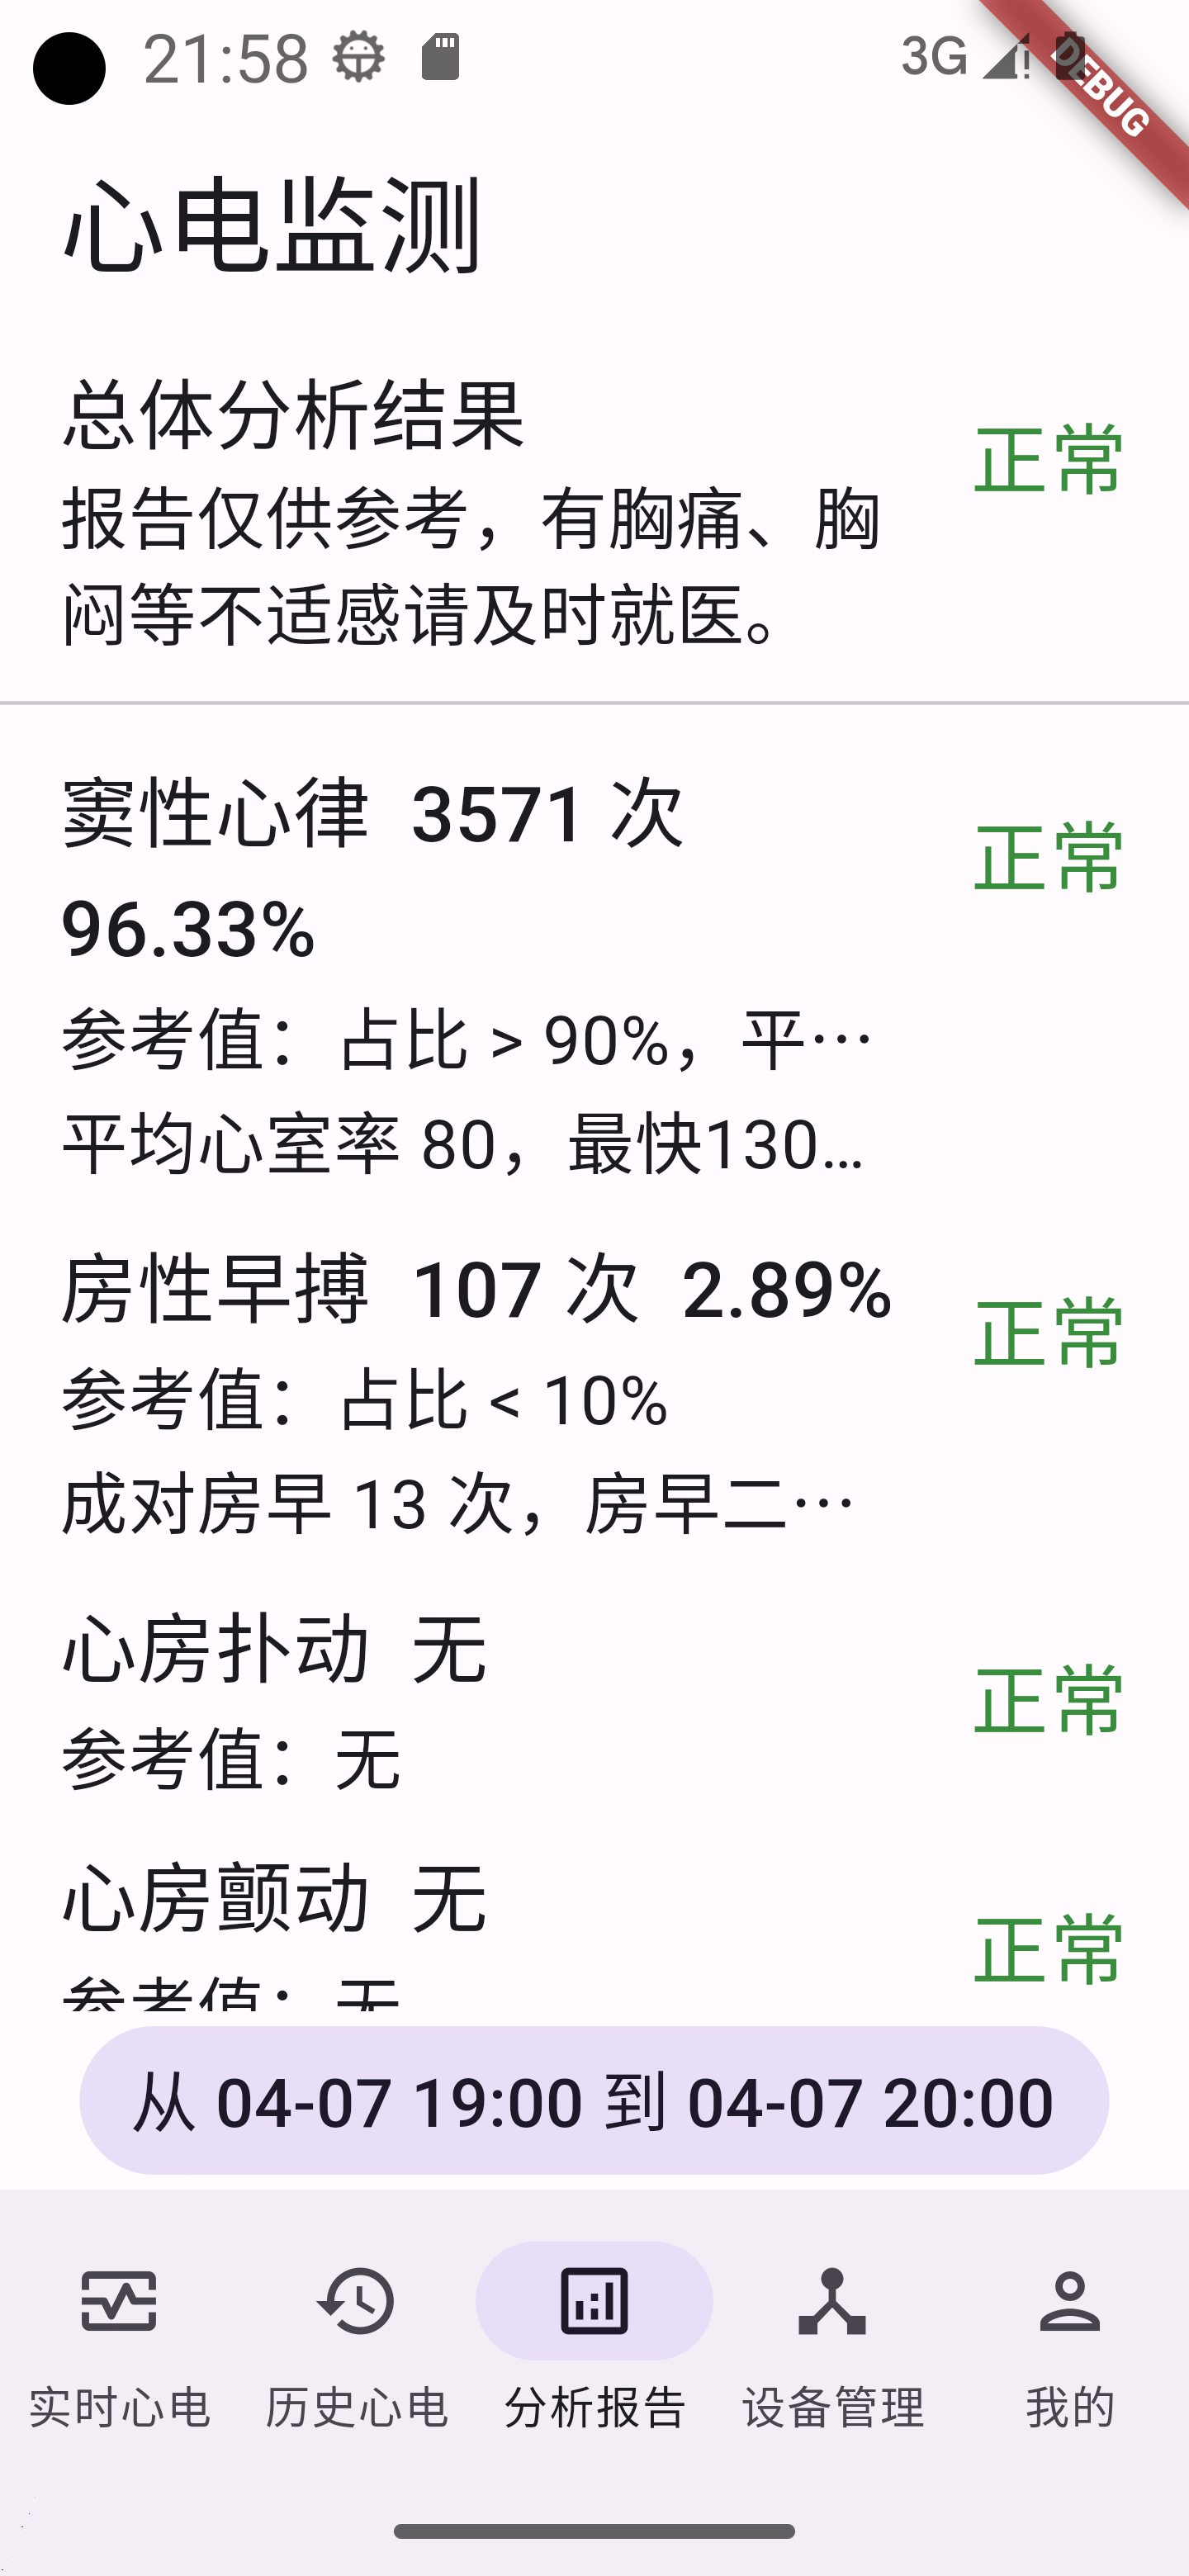
\includegraphics[width=.33\textwidth]{../assets/big}}
    \subcaptionbox{粗体高对比度}{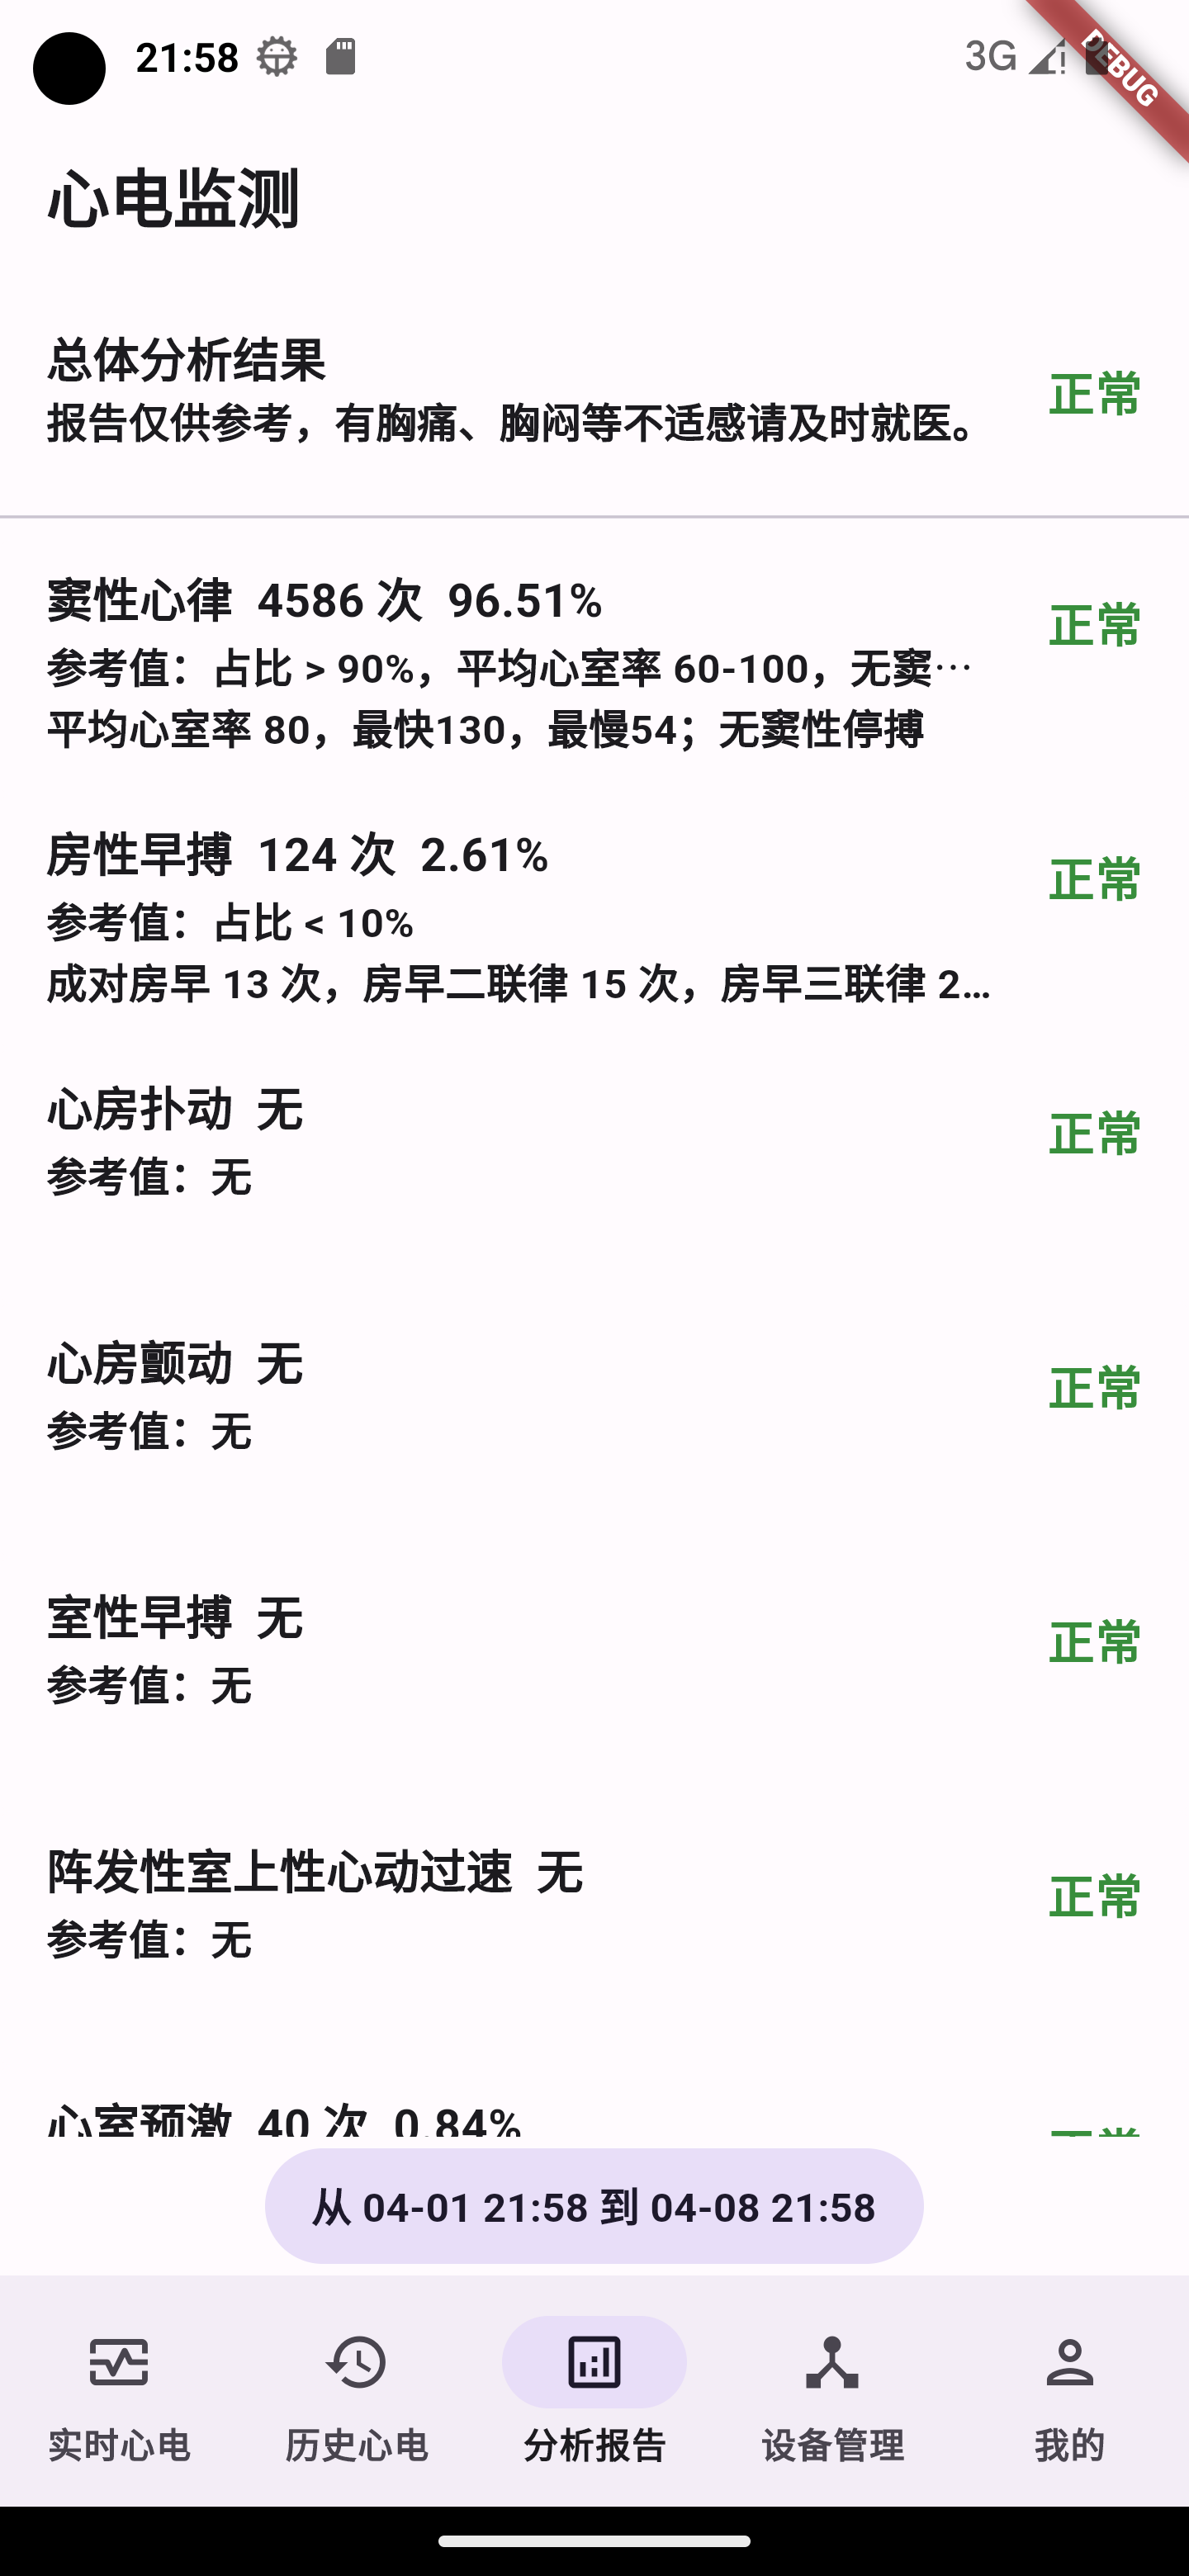
\includegraphics[width=.33\textwidth]{../assets/bold}}
    \subcaptionbox{深色模式}{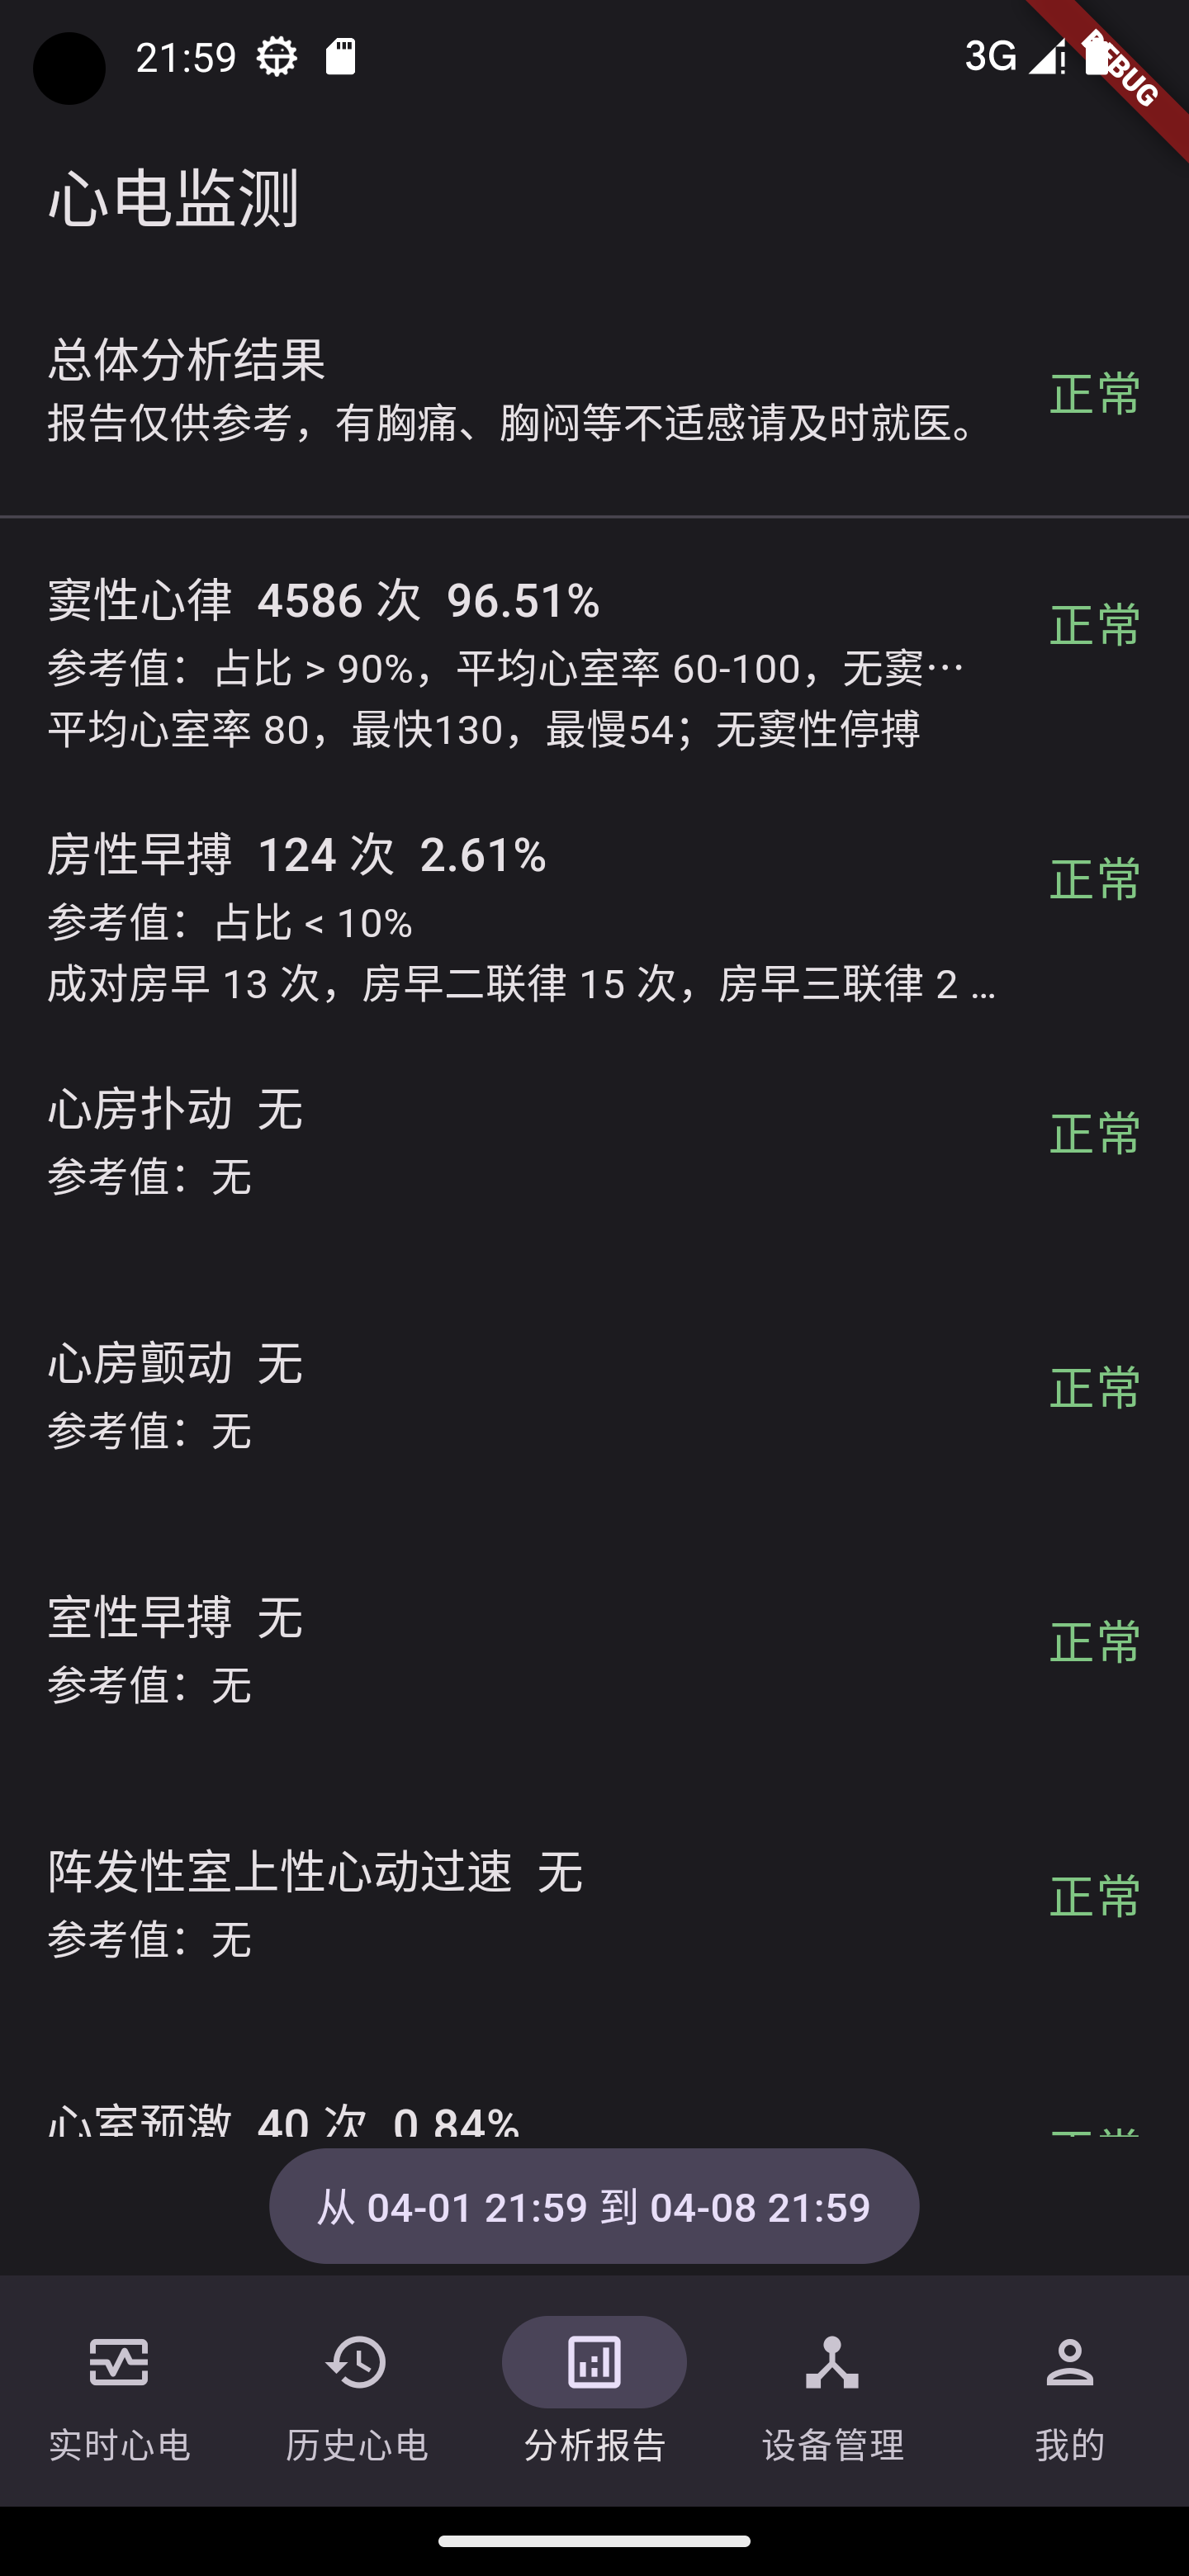
\includegraphics[width=.33\textwidth]{../assets/dark}}
    \bicaption{应用的无障碍设计}{Accessibility design of the app}
    \label{fig:accessibility}
\end{figure}

当用户开启了界面放大后,应用内一些原本在一行之内显示的文本会无法在一行内完整显示。对于有必要完全显示出来的内容,应用会将其进行换行,在多行之中显示。对于没有必要完全显示的内容,应用会将其折叠,以省略号指示内容未显示完全。通过这些设计,应用在界面放大的状态下虽然美观程度略有下降,但功能都可以保证正常使用。界面放大的一个常用替代方式是将文本加粗加黑,应用在这种情况下也可以正常提供功能。

为了支持深色模式与浅色模式的切换,应用在设计中尽量避免了使用固定的颜色,而是使用系统上下文提供的颜色。这样,应用在不同的主题下自然都可以随之自动切换颜色,从而正常显示内容。


\section{应用的数据库设计}\label{sec:db-design}

应用的数据库分为两部分,存储简单数据的SharedPreferences数据库和存储复杂数据的Isar数据库。前者主要用于存储应用的设置,后者主要用于存储历史心电数据与分析报告结果。

\subsection{SharedPreferences数据库的设计}\label{subsec:shared-preferences}

\subsubsection{SharedPreferences数据库介绍}\label{subsubsec:shared-preferences-intro}

SharedPreferences是Flutter的一个包,提供了简单键值对的存储功能,可以视为一个键值型的非关系型数据库。其在Android平台上基于同名的SharedPreferences功能,在iOS上则基于NSUserDefaults功能。

SharedPreferences仅支持少数几种数据类型,即 |int|、|double|、|bool|、|String| 以及 |List<String>|。键值型数据库的读写非常简单,不需要进行特别的设计。本项目对该数据库的设计主要在于将各种需要存储的类型映射为其支持的类型。

\subsubsection{Duration类型的存储}\label{subsubsec:duration-storage}

Duration类型表示时间长度。由于应用内对时间的各种操作最多只需要毫秒精度,所以应用在需要将Duration类型的数据存入SharedPreferences时会将其转换为毫秒数以整数格式进行存储。在读取时,应用会将毫秒数转换为Duration类型。

\subsubsection{Color类型的存储}\label{subsubsec:color-storage}

Color类型表示颜色。应用在需要将Color类型的数据存入SharedPreferences时,会将其编码为32位整数以整数格式进行存储。在读取时,应用会将32位整数转换为Color类型。具体的编码方式是将颜色的ARGB值分别存储在32位整数的高8位、次高8位、次低8位和低8位中。

\subsubsection{枚举类型的存储}\label{subsubsec:enum-storage}

应用中使用了各种枚举类型,有时会需要将枚举类型存入SharedPreferences。应用在存储枚举类型时会将其转换为索引值,以整数形式存储。枚举类型常见的存储方式还包括按其名称以字符串形式存储、为每个枚举值赋予自定义值然后按自定义值的类型存储。相比其他方法,直接按索引值存储的优点在于其简单高效;缺点在于已经存在的枚举值不能轻易改动,否则会破坏已有的数据。由于应用内的枚举值设计基本不变,所以该缺点并不明显,可以接受。

\subsection{Isar数据库的设计}\label{subsec:isar}

\subsubsection{Isar数据库介绍}\label{subsubsec:isar-intro}

Isar是Flutter的一个包,提供了一个跨平台数据库。Isar属于非关系型数据库,不过提供了组合索引、ACID语义、事务等功能,可以视为一个关系型数据库的子集。相比常规的关系型数据库,Isar有一些额外的限制(或者说缺少一些功能)影响了本应用对数据库的设计。

当使用Isar来存储数据时,需要对Collection进行操作。Collection可理解为Isar数据库中的表,其包含的数据只能为同一类Dart对象,每个对象则代表了对应数据表中的一行数据。该类对象所对应的类则是这张表的Schema,其中每个字段对应数据库中的一列。与一般的关系型数据库相同的是,Schema中必须要有主键;不同的是,Isar中主键的类型被限制为64位整数值,这一限制导致了本应用对数据库的设计中的一些不同之处。

在查询时,Isar并不像一般的关系型数据库那样在编写SQL语句后自动生成最优查询策略,而是需要手动指定查询方式。Isar中的查询过滤方式分为两种,分别称为Filter和Where,前者执行遍历过滤,后者依靠索引表进行过滤。多个Where子句的过滤结果直接只能进行并集运算,无法进行交集运算。如果需要按多个属性进行过滤,并且还希望使用索引加快速度,就必须使用组合索引。组合索引有一个特殊的限制:主键不能包含在组合索引之中。这一限制也影响了本应用对数据库的设计。

此外,Isar对外键、Join等功能的支持也比较有限,不过这些功能在本应用的数据库设计中本来也不需要,所以不进行过多说明。

\subsubsection{心拍数据的存储}\label{subsubsec:beat-storage}

在分析报告数据中,只有心拍数据被存入数据库,基于心拍数据产生的进一步分析结果则只在查询时动态生成。这一方面是因为算法的大部分时间开销在于分割分类模型的运行上,其余部分开销较小。另一方面是因为心拍之外的结果的格式较为复杂,不方便进行合适的数据库设计。心拍数据则格式简单,且存储、查询时可以对多段数据进行拼接、裁剪而不失去太多准确度,所以适合存入数据库之中。

心拍数据的Schema包含3个字段和2个索引。字段中的ID是由Isar管理的自增整数,没有特别用途。另外两个字段分别是DateTime类型的心拍时间和枚举类型的心拍类型标签。对心拍时间进行了单列索引,以方便在查看历史心电时快速检索指定时间范围内的所有心拍。对心拍类型和心拍时间进行了组合索引,以心拍类型为主索引,这个组合索引用于查询指定标签在指定时间范围内的数量等信息。

\subsubsection{心电数据的存储}\label{subsubsec:point-storage}

对心电数据的查询需求较为简单,只有在历史心电界面中需要对指定时间范围内的心电数据进行查询。因此,也只需要在心电数据的时间上进行索引。

由于没有组合索引的需求,所以可以直接把时间作为主键,以节省额外的索引表的开销,并避免浪费主键所占的空间。由于主键只能为64位整数,所以需要对时间进行编码。考虑到时间只需要毫秒精度,将其编码为了自Unix纪元(UTC时间的1970年1月1日00:00:00)以来经过的毫秒数。这样,心电数据的Schema中不包含任何额外定义的索引,查询时只使用主键自带的索引功能。

除了作为主键的时间之外,一条心电数据中还包含各导联的电压数据。由于导联I、II、III被定义为左臂、右臂、左腿三个点之间的电位差,这三个导联的数据实际上只包含两个差值的信息量,所以只需要存储两个值即可。
